%# -*- coding:utf-8 -*-
%!TEX root = ../mainxb.tex


\setcounter{page}{1}
\chapter{函数的基本性质} % {第3章校本作业}

\section{函数基本概念}

\zsd 函数的概念、定义域、值域、相同的函数. 

% todo: T6图. 
A组: 
\begin{enumerate}
\item $y = \dfrac{1}{x}$的定义域为\blkda[2]{$\{x | x \neq 0\}$}.
\begin{jieda}
分母不为0.
\end{jieda}

\item $y = \sqrt{x}$的定义域为\blkda[2]{$\{x | x \geq 0\}$}.
\begin{jieda}
根式下非负.
\end{jieda}

\item $y = (2x+1)^0$的定义域为\blkda[2]{$\{x | x \neq -\dfrac{1}{2}\}$}.
\begin{jieda}
$0^0$没有意义.
\end{jieda}

\item 函数$y=f(x)$的图像与直线$x=a$的公共点的数目是\dotfill(\kh{C})
\xx{1}{0}{0或1}{1或2}
\begin{jieda}
当$a$在$f(x)$的定义域中时, 函数$f(x)$的图像与直线$x=a$只有一个交点; \\
当$a$不在$f(x)$的定义域中时, 函数$f(x)$的图像与直线$x=a$无交点.\\
故选C.
\end{jieda}

\item 下列图像中可以作为函数$y=f(x)$的图像的是\dotfill(\kh{D})
\begin{minipage}{\linewidth}
\centering

\includegraphics[height=5\baselineskip]{./bodyxb/src/bx01ch03sec1hanshujibengainianA5a.png}\qquad

\includegraphics[height=5\baselineskip]{./bodyxb/src/bx01ch03sec1hanshujibengainianA5b.png}\qquad

\includegraphics[height=5\baselineskip]{./bodyxb/src/bx01ch03sec1hanshujibengainianA5c.png}\qquad

\includegraphics[height=5\baselineskip]{./bodyxb/src/bx01ch03sec1hanshujibengainianA5d.png}
\end{minipage}

\end{enumerate}


B组: 
\begin{enumerate}
\item 函数$f(x)=\dfrac{\sqrt{4-x^2}}{x-1}$的定义域是\blkda[3]{$[-2,1)\cup(1,2]$}.
\begin{jieda}
由题意有 
$\begin{cases}
4-x^2\geq 0\\
x-1\neq 0\\
\end{cases}$, 
解得$x\in[-2,1)\cup(1,2]$.
\end{jieda}


\item 函数$f(x)=\dfrac{(x+1)^0}{\sqrt{|x|-x}}$的定义域是\blkda[3]{$(-\infty, -1) \cup (-1, 0)$}.
\begin{jieda}
根式里非负以及分母不为零要求$x < 0$；分子上要求$x \neq -1$，综上得到$x \in (-\infty, -1) \cup (-1, 0)$ \\
\ps 学生容易忽视分母上不为零的约束，只判断了$|x| - x \geq 0$恒成立，由此得到的答案为$(-\infty, -1) \cup (-1, 0]$
\end{jieda}

\item 已知下列各组函数, 其中是同一函数的是\blkda{\ding{175} \ding{177}}:
\begin{dingautolist}{172}
\item $y = \dfrac{(x+3)(x-5)}{x+3}, y = x-5$; 
\item $y = \sqrt{x+1} \cdot \sqrt{x-1}, y = \sqrt{(x+1)(x-1)}$; 
\item $f(x) = x, g(x) = \sqrt{x^2}$; 
\item $f(x) = \sqrt[3]{x^4-x^3}, F(x) = x\sqrt[3]{x-1}$;
\item $f_1(x) = (\sqrt{2x-5})^2, f_2(x) = 2x-5$
\item $f(x) = x^0, g(x) = \dfrac{1}{x^0}$
\end{dingautolist}

\item 若函数$y=\sqrt{(a^2-1)x^2+(a-1)x+\dfrac{2}{a+1}}$的定义域为$\bR$, 则实数$a$的取值范围是\blkda{$[1,9]$}. 
\begin{jieda}
$\iff (a^2-1)x^2+(a-1)x+\dfrac{2}{a+1}\geq 0$恒成立. 显然$a\neq -1$, 故分为以下几种情况讨论. 
\begin{enumerate}[(1)]
\item $a=1$时, 显然成立; 
\item $a\neq\pm1$时, 有$a^2-1>0$且$\Delta\leq 0$, 解得$a\in(1,9]$. 
\end{enumerate}
综上, $a\in[1,9]$. 
\end{jieda}

\item 下列函数中, 表示同一函数的是\dotfill(\kh{B})
\xx{$f(x)=\dfrac{x^2-9}{x-3}$与$g(x)=x+3$}
{$y=\dfrac{x^2}{\abs{x}}(x\neq 0)$与$f(t)=\begin{cases}
t, & t>0\\
-t, & t<0
\end{cases}$}
{$f(x)=\dfrac{\sqrt{x}}{\sqrt{x+1}}$与$g(x)=\sqrt{\dfrac{x}{x+1}}$}
{$f(x)=\sqrt{(2x-1)^2}$与$g(t)=2t-1$}
\begin{jieda}
函数的两要素: 定义域, 对应法则. 先看定义域; 表现形式可以不同(实质上等价); 字母可以不同(函数的关键在于对应法则是什么). 
\end{jieda}

\item 已知函数$f(x)=\dfrac{\sqrt[3]{3x-1}}{ax^2+ax-3}$的定义域为$\bR$, 则实数$a$的取值范围是\dotfill(\kh{B})
\xx{$a>\dfrac{1}{3}$}
{$-12<a\leq 0$}
{$-12<a<0$}
{$a\leq\dfrac{1}{3}$}
\begin{jieda}
$ax^2+ax-3=0$无解. (1) $a=0$, 可; (2) $a\neq 0$时, $\Delta<0$, 即$a\in(-12,0)$. 综上, $a\in(-12,0]$. 
\end{jieda}

\item 求下列函数的定义域: 
\begin{enumerate}
\item $y=\dfrac{\sqrt{x-4}}{\abs{x}-5}$ \hfill \blkda[4]{$ [4,5)\cup(5,+\infty)$}
\item $y=\dfrac{x}{2x-\sqrt{3-x}}$ \hfill \blkda[4]{$\left(-\infty,\dfrac{3}{4}\right)\cup\left(\dfrac{3}{4},3\right]$}
\item $y=\sqrt{x^2-5x+6}+\dfrac{(x-1)^0}{\sqrt{x+\abs{x}}}$ \hfill \blkda[4]{$(0,1)\cup(1,2]\cup[3,+\infty)$}
\end{enumerate}
\begin{jieda}
\ps 第二小问学生易在计算$2x=\sqrt{3-x}$时直接平方后得到$-1$和$\dfrac{3}{4}$, 导致答案为$\left(-\infty,-1 \right)\cup\left(-1,\dfrac{3}{4}\right)\cup\left(\dfrac{3}{4},3\right]$ 正确的逻辑关系为：$f(x) = \sqrt{g(x)} \Leftrightarrow \left \{ \begin{array}{l}
     f(x) \geq 0  \\
     (f(x))^2 = g(x)
\end{array} \right.$
\end{jieda}



\item 设$x_1,x_2$是关于$x$的一元二次方程$x^2-2(m-1)x+m+1=0$的两个实根, 求$y=x_1^2+x_2^2$的解析式(用含字母$m$的式子表示). 
\begin{jieda}
前提是$\Delta\geq 0$, 解得$m\in(-\infty,0]\cup[3,+\infty)$. \\
于是$y=(x_1+x_2)^2-2x_1x_2=4m^2-10m+2$. 
\end{jieda}
\begin{vspace_}
\vsp[7]
\end{vspace_}

\item 设函数$f(x)=\sqrt{-x^2+2x+8}$的定义域为$A$, 函数$g(x)=\dfrac{1}{\sqrt{1-\abs{x-a}}}$的定义域为$B$, 
且$A\cap B=\varnothing$, 求实数$a$的取值范围. 
\begin{jieda}
易得$A=[-2,4]$, $B=(a-1,a+1)$. \\
又$A\cap B=\varnothing$, 于是$a+1\leq-2$或$a-1\geq 4$, 即$a\leq-3$或$a\geq 5$. \\
\ps 如果上述解法不理解, 可以从反面即$A\cap B\neq\varnothing$来考虑. 
\end{jieda}
\begin{vspace_}
\vsp[7]
\end{vspace_}
\clearpage

\item 设函数$f(x)=\dfrac{1}{\sqrt{ax^2+ax+1}}$分别满足下列条件, 求实数$a$的取值范围: 
\begin{enumerate}
\item 定义域恰是$(-2,1)$; 
\item 定义域是$\mathbf{R}$; 
\item 值域是$(0,+\infty)$. 
\end{enumerate}
\begin{jieda}
\begin{enumerate}
    \item 定义域恰是$(-2,1)$即$ax^2+ax+1>0$的解集为$(-2,1)$. 因此对应方程$ax^2+ax+1=0$的两根为$-2, 1$，将$1$代入方程可以解得$a = -\dfrac{1}{2}$，因此$a$的取值范围是$\{-\dfrac{1}{2}\}$
    
    \item $ax^2+ax+1>0$恒成立. \\
    $a=0$时显然成立; \\
    $a\neq 0$时, $a>0$且$ \Delta<0$, 即$a\in(0,4)$. \\
    故$a\in[0,4)$. 
    
    \item 问题等价于$y=ax^2+ax+1$的值域包含$(0,+\infty)$. \\
    $a=0$显然不符合条件; \\
    $a\neq 0$时, $a>0$且$\Delta\geq0$, 即$a\geq 4$. \\
    故$a\geq 4$. \\
    \ps 学生容易犯两类错误：\\
        1. 误认为当$\sqrt{ax^2+ax+1}$的定义域是$\mathbf{R}$时，其值域是$(0, +\infty)$，从而错误地将问题转化为$\sqrt{ax^2+ax+1}$的定义域是$\mathbf{R}$，要求对应的二次函数开口向上且$\Delta < 0$，得到$[0, 4)$\\
        2. 计算$\Delta \geq 0$之后忘记开口方向的约束，得到$(-\infty, 0] \cup [4, +\infty)$
\end{enumerate}
\end{jieda}
\begin{vspace_}
\vsp[5]
\end{vspace_}

\item 已知函数$f(x) = \dfrac{2x}{x+1}$
\begin{enumerate}
\item 设$a \neq 0$且$a \neq -1$，求$f(a) + f(\dfrac{1}{a})$的值; 
\item 求$f(1) + f(2) + \cdot \cdot \cdot + f(100) + f(\dfrac{1}{2}) + f(\dfrac{2}{2}) + \cdot \cdot \cdot + f(\dfrac{100}{2}) + f(\dfrac{1}{3}) + f(\dfrac{2}{3}) + \cdot \cdot \cdot + f(\dfrac{100}{3}) + f(\dfrac{1}{4}) + f(\dfrac{2}{4}) + \cdot \cdot \cdot + f(\dfrac{100}{4}) + \cdot \cdot \cdot + f(\dfrac{1}{100}) + f(\dfrac{2}{100}) + \cdot \cdot \cdot + f(\dfrac{100}{100})$的值. 
\end{enumerate}
\begin{jieda}
\begin{enumerate}[(1)]
\item 易得$f(a)+f(\frac{1}{a})=\dfrac{2a}{a+1}+\dfrac{\frac{2}{a}}{\frac{1}{a}+1}=\cdots=2$. 
\item 对应$\dfrac{i}{j}$而已, 当$i,j$遍历了$1-100$时, $\dfrac{j}{i}$也遍历了对应的情形, 且与$\dfrac{i}{j}$一一对应. \\
两者配对之和为$2$，共有$5000$对，故所求为$10000$. 
\end{enumerate}
\ps 其实也可以从有序实数对$(i,j)$与$(j,i)$的角度理解. 
\end{jieda}
\begin{vspace_}
\vsp[5]
\end{vspace_}

\item 已知$f(x) = \dfrac{kx+1}{k^2x^2 + 3kx + 2}$
\begin{enumerate}
    \item 若$k=2$，求函数$y = f(x)$的定义域
    \item 若函数$y = f(x)$的定义域为$\mathbf{R}$，求实数$k$的值
\end{enumerate}

\begin{jieda}
\begin{enumerate}[(1)]
\item $f(x) = \dfrac{2x+1}{4x^2+6x+2}$，故$4x^2+6x+2 \neq 0$，因此定义域为$\{x|x \neq -\dfrac{1}{2} \mbox{且} x \neq -1\}$
\item 
\begin{enumerate}
    \item 当$k = 0$时，满足函数定义域为$\mathbf{R}$.
    \item 当$k \neq 0$时，应有$\Delta = 9k^2 - 8k^2 = k^2 < 0$，没有满足条件的$k$
\end{enumerate}
综上，$k = 0$
\end{enumerate}
\end{jieda}
\begin{vspace_}
\vsp[5]
\end{vspace_}

\item 已知定义域为$\mathbf{R}$的函数$y = f(x)$满足：\ding{172} $f(a+b) = f(a)f(b)$对任何实数$a, b$都成立； \ding{173} 存在实数$x_1, x_2$使得$f(x_1) \neq f(x_2)$，求证：
\begin{enumerate}
    \item $f(0) = 1$
    \item $f(x) > 0$
\end{enumerate}

\begin{jieda}
证明: 
\begin{enumerate}
    \item 令$a = 0$，故对任意$b$有$f(b) = f(b) \cdot f(0)$，又因为存在实数$x_1, x_2$使得$f(x_1) \neq f(x_2)$，故$f(x)$不恒为0，因此有$f(0) = 1$.
    \item 因为$f(a+b) = f(a)f(b)$对任何实数$a, b $都成立，故$f(a) = [f(\dfrac{a}{2})]^2 \geq 0$恒成立.此外，$1 = f(0) = f(a) \cdot f(-a)$.若存在$f(a_0) = 0$，则该式不满足.\\
    故$f(x) \neq 0$恒成立.综上，$f(x) > 0$恒成立.
\end{enumerate}
\end{jieda} 
\begin{vspace_}
\vsp[6]
\end{vspace_}

\end{enumerate}

C组: 
\begin{enumerate}
\item 已知集合$A = \{n | \dfrac{3^n + 4^n}{5} \in \mathbf{N^*}, n \in \mathbf{N^*} \}$，集合$B =\{t | t = (2k-1)^2+1, k \in \mathbf{N^*} \}$，则集合$A$与集合$B$的关系是\blkda[2]{$B \subset A$}.

\begin{jieda}
$3^n$的个位数分别为3,9,7,1, 且以4为周期; $4^n$的个位数为4,6, 且周期为2.\\
所以$A=\{n\mid n=4k-2,n\in\mathbb{N^*}\}$.\\
而$(2k-1)^2+1=4(k^2-k+1)-2$, 故$B\subseteq A$.\\
又$k^2-k+1$只能是奇数, 故$B\subsetneqq A$.
\end{jieda}

\begin{vspace_}
\vsp[6]
\end{vspace_}

\item 已知集合$A = \{a_1, a_2, a_3, \cdot \cdot \cdot, a_n \} ( n \geq 3, n \in \mathbf{N^*})$，集合$B =\{a_i + a_j | a_i \in A, a_j \in A, 1 \leq i < j \leq n \}$，则集合$B$中元素个数的最小值为\blkda[2]{$2n-3$}（用$n$的代数式表示）.

\begin{jieda}
不妨设$a_1 < a_2 < a_3 < ... < a_n$\\
此时必有$a_1+a_2 < a_1 + a_3 < ... < a_1 + a_n < a_2 + a_n < a_3 + a_n < ... < a_{n-1} + a_n$.\\
在这个不等关系中共有$2n-3$个元素，故$B$中元素个数$|B| \geq 2n-3$.\\
当$a_1, a_2, a_3, ..., a_n$构成公差非0的等差数列时，$a_m + a_n = a_p + a_q (m+n = p+q)$，必有$B$中元素个数为$2n-3$
\end{jieda} 
\end{enumerate}
\clearpage

\section{函数基本概念(2)} % {3.1.1 函数}
\zsd 函数的概念、定义域、值域、相同的函数. 

% todo: T6图. 
A组: 
\begin{enumerate}

\item 函数$y = f(x)$的定义域为$[-1, 1]$，则函数$y = f(3x-2)$的定义域为\blkda{$[\dfrac{1}{3}, 1]$}.
\begin{jieda}
$3x-2 \in [-1, 1], 3x \in [1, 3], x \in [\dfrac{1}{3}, 1]$
\end{jieda} 

\item 将$y = |x-1| + |x+2|$改为分段函数形式\blkda[5]{$y = \left \{ \begin{array}{ll}
    -1-2x & x < -2 \\
    3 & -2 \leq x \leq 1 \\
    2x+1 & x > 1
\end{array} \right.$}

\begin{jieda}
分类讨论去绝对值即可.
\end{jieda} 

\item 定义域为$\bR$的函数$y=f(x)$的值域为$[a,b]$, 则函数$y=f(x+a)$的值域为\dotfill(\kh{B})
\xx{$[2a,a+b]$}{$[a,b]$}{$[0,b-a]$}{$[-a,a+b]$}
\begin{jieda}
这是求值域. 函数图像的水平平移对值域一点儿影响都没有. \mydate{20221025}
\end{jieda}

\item 函数$y=x^2-2x$的定义域为$\{0,1,2,3\}$, 那么值域为\blkda{$\{-1,0,3\}$}.
\begin{jieda}
将自变量的值逐个代入解析式, 求得值域为$\{-1,0,3\}$.
\end{jieda}

\item 函数$y=\sqrt{1-x}+\sqrt{x+3}$的值域是\blkda{$[2,2\sqrt{2}]$}.
\begin{jieda}
首先$1-x\geq0$且$ x+3\geq 0$, 即$x\in[-3,1]$. \\
其次$y^2=1-x+x+3+2\sqrt{(1-x)(x+3)}=4+2\sqrt{-(x+1)^2+4}\in[4,8]$, 
故$y\in[2,2\sqrt{2}]$. \\
\ps 利用算数平均数小于等于平方平均数可以验证最值：$y \leq \sqrt{2} \sqrt{1-x + x + 3} = 2\sqrt{2}$，
\end{jieda}

\item 请写出$y = \dfrac{3+x}{4-x}$的对称中心， 定义域， 值域.
\begin{jieda}
$y = \dfrac{3+x}{4-x} = -1 + \dfrac{7}{4-x} = -(\dfrac{7}{x-4} + 1)$ \\
故对称中心为$(4, -1)$，定义域为$(-\infty, 4) \cup (4, +\infty)$，值域为$(-\infty, -1) \cup (-1, +\infty)$
\end{jieda}
\begin{vspace_}
    \vsp[3]
\end{vspace_}

\end{enumerate}


B组: 
\begin{enumerate}
    \item 设函数$f(x)=\begin{cases}
2x(x+3), & x\geq 0\\
2x(3-x), & x<0
\end{cases}$, 
则$f(a)$=\blkda[2.5]{$2a\abs{a}+6a$}. 
\begin{jieda}
是否要合并为一个式子? 未必. 只是不想敲很多字符而已. 
\end{jieda}

\item 已知函数$f(x)=\begin{cases}
x-3, & x\geq 10\\
f(f(x+5)), & x<10\\    
\end{cases}$, 
则$f(7)$=\blkda{8}.
\begin{jieda}
\begin{align*}
f(7) & =f(f(7+5))=f(f(12))\\
& =f(12-3)=f(9)\\
& =f(f(9+5))=f(f(14))\\
& =f(14-3)=f(11)\\
& =11-3=8.
\end{align*}
更为一般的情形, 分段讨论如下: 当$x\in[8,10)$时, 
\begin{align*}
f(x) & = f(f(x+5)) & \hspace*{1cm} x+5\in[13,15)\\
& = f(x+5-3)=f(x+2) & \hspace*{1cm} x+2\in[10,12)\\
& = x+2-3=x-1 & 
\end{align*}
当$x\in[6,8)$时, 
\begin{align*}
f(x) & = f(f(x+5)) & \hspace*{1cm} x+5\in[11,13)\\
& = f(x+5-3)=f(x+2) & \hspace*{1cm} x+2\in[8,10)\\
& = (x+2)-1=x+1
\end{align*}
于是不难得到: 当$x\in[2k,2k+2)$时, $f(x)=f(f(x+5))=f(x+5-3)=f(x+2)$. 其中$k\zz,k\leq 4$. 
\end{jieda}

\item 若函数$y=f(x)$的定义域是$[0,2]$, 则函数$g(x)=\dfrac{f(2x)}{x-1}$的定义域为\blkda{$[0,1)$}. 
\begin{jieda}
$2x\in[0,2]$且$ x-1\neq 0$. 
\end{jieda}

\item 已知函数$f(x)=\begin{cases}
(x+1)^2, & x<1\\
4-\sqrt{x-1}, & x\geq 1
\end{cases}$, 
则使得$f(x)\geq 1$的$x$的取值范围是\blkda[3]{$(-\infty,-2]\cup[0,10]$}. 
\begin{jieda}
分段函数分段求, 还要作何打算. 
\ps 错误率非常高
\end{jieda}

\item 若$0<x<4$, $\gauss{x}$表示不超过$x$的最大整数，则方程$x^2-2\gauss{x}-x=0$的解为\blkda[3]{$\dfrac{1+\sqrt{17}}{2},3$}. 
\begin{jieda}
一般来说用$\gauss{x}\leq x<\gauss{x}+1$放缩, 以本题为例, 先得到$x^2-x=2\gauss{x}$. \\
于是$2(x-1)<x^2-x\leq 2x$, 故$x\in[0,1)\cup(2,3]$. \\
当$x\in[0,1)$时, $\gauss{x}=0$, 于是$x^2-x=0$, 解得$x=0$; \\
当$x\in(2,3)$时, $\gauss{x}=2$, 于是$x^2-x=4$, 解得$x=\dfrac{1+\sqrt{17}}{2}$; \\
当$x=3$时, $\gauss{x}=3$, 于是$x^2-x=6$, 解得$x=3$. \\
综上, 考虑到$x\in(0,4)$, 故解为$\dfrac{1+\sqrt{17}}{2},3$. \\
\ps 上述3种情形中, 需要注意前面的范围. 这样的做法就是把$\gauss{x}$中的$\gauss{\quad}$去掉, 与去绝对值之类的东西一个意思. 
\end{jieda}

\item 国家规定个人稿费纳税办法是: 不超过800元的不纳税; 超过800元而不超过4000元的按超过800元部分的14\% 纳税; 
超过4000元的按全部稿酬的11\% 纳税. 已知某人出版一本书, 共纳税420元, 这个人应得稿费(扣税前)为\dotfill(\kh{C})
\xx{2800元}{3000元}{3800元}{3818元}
\begin{jieda}
$y=\begin{cases}
0, & 0\leq x\leq 800\\
0.14(x-800), & 800<x\leq 4000\\
0.14(4000-800)+0.11(x-4000), & x>4000
\end{cases}$. 
\end{jieda}
\clearpage
\item 某学生离家去学校, 为了锻炼身体, 一开始跑步前进, 跑累了再走余下的路程. 下图中, 纵轴表示离学校的距离, 横轴表示出发后的时间, 
则下列四个图形中较符合该学生的走法是\dotfill(\kh{D})

\begin{figure}[h]
    \centering
    
\includegraphics[width=0.75\linewidth]{bodyxb//src/bx01ch03sec2hanshujibengainianB7.png}
\end{figure}

\item 已知函数$y=f(x+1)$的定义域为$[-2,3]$, 则$y=f(2x-1)$的定义域为\blkda{$\left[0,\dfrac{5}{2}\right]$}.
\begin{jieda}
因为$x\in[-2,3]$, 所以$x+1\in[-1,4]$.\\
故对$y=f(2x-1)$有$2x-1\in[-1,4]$, 解得$x\in\left[0,\dfrac{5}{2}\right]$.
\end{jieda}

\item 设函数$f(x)=\begin{cases}
x^2+bx+c, & x\leq 0\\
2, & x>0
\end{cases}$, 
若$f(-4)=f(0)$, $f(-2)=-2$, 则方程$f(x)=x$的解集为\blkda{$\{-2,-1,2\}$}.
\begin{jieda}
$16-4b+c=2$且$ 4-2b+c=-2$, 故$(b,c)=(4,2)$. \\
于是$\begin{cases}
x\leq 0\\
x^2+4x+2=x
\end{cases}$, 或$\begin{cases}
x>0\\
2=x
\end{cases}$, 解得$x=-2,-1,2$. 
故解集为$\{-2,-1,2\}$
\end{jieda}

\item 若一系列函数的解析式相同, 值域相同, 但其定义域不同, 则称这些函数为``同族函数'', 
那么函数解析式为$f(x)=x^2$, 值域为$\{1,4\}$的``同族函数''共有\blkda{$9$}个.
\begin{jieda}
$1,-1,\pm1\to 1$, $2,-2,\pm2\to 4$, 于是从值域的角度, $x$的组合共有$3\times3=9$种选择. \\
\ps 此题错误率非常高，分成两种情况。1. 学生没有乘法原理的概念，采用列举法时候出错；2. 学生忽视可以取两个自变量对应于一个函数值的情况。
\end{jieda} 

\item 
\begin{enumerate}
\item 求函数$y=\abs{x-1}+\abs{x+2}$的值域并作出其大致图像; 
\item 求函数$y=\abs{x^2-2x-3}$的值域并作出其大致图像. 
\end{enumerate}
\begin{jieda}
(1) $[3,+\infty)$, 分段作图, 图略; (2) $[0,+\infty)$(显然), 图略. (ggb输入解析式即得)
\end{jieda}
\begin{vspace_}
\vsp[3]
\end{vspace_}

\item 定义符号函数$\sgn x=\begin{cases}
1,  & x>0\\
0,  & x=0\\
-1, & x<0\\
\end{cases}$,
解不等式$x+2>(x-2)^{\sgn x}$. 
\begin{jieda}
等价于(1)$\begin{cases}
x<0\\
x+2>(x-2)^{-1}
\end{cases}$
(2)$\begin{cases}
x=0\\
x+2>(x-2)^0
\end{cases}$
(3)$\begin{cases}
x>0\\
x+2>x-2
\end{cases}$. \\
解得(1)$x\in(-\sqrt{5},0)$; (2)$x=0$; (3)$x>0$. \\
综上, 解集为$(-\sqrt{5},+\infty)$. 
\end{jieda}

\begin{vspace_}
\vsp[3]
\end{vspace_}

\item 已知$f(x) = \left \{ \begin{array}{ll}
     x^2 - 1 & |x| \leq 1 \\
     1 & |x| > 1
\end{array}\right.$，
\begin{enumerate}
    \item 画出函数$y = f(x)$的大致图像并求$y = f(x)$的定义域和值域；
    \item 对于实数$a$，求$f(a^2+1)$的值.
\end{enumerate}

\begin{jieda}
\begin{enumerate}
    \item 图略.定义域为$\mathbf{R}$，值域为$[-1, 0] \cup \{1\}$
    \item 若$a = 0$，则$f(a^2+1) = f(1) = 0$；若$a \neq 0$，则$f(a^2+1) = 1$
\end{enumerate}
\end{jieda}

\begin{vspace_}
\vsp[3]
\end{vspace_}

\item 已知函数$f(x)=\begin{cases}
-2x^2+2x+\frac{1}{2}, & 0\leqslant x<\frac{1}{2}\\
-2x+2, & \frac{1}{2}\leqslant x\leqslant 1\\
\end{cases}$.
\begin{enumerate}[(1)]
\item 在平面直角坐标系中画出函数$y=f(x)$的图像;
\item 当$x_1\in\left[0,\frac{1}{2}\right)$时, $f(x_1)=x_2$, 且$f(x_2)=x_1$, 求$x_1, x_2$的值. 
\end{enumerate}
\begin{jieda}
\begin{enumerate}[(1)]
\item 略. 

\item 当$x_1\in\left[0,\frac{1}{2}\right)$时, $x_2=f(x_1)\in\left[\dfrac{1}{2},1\right)$, 故$f(x_2)=-2x_2+2$. \\
于是$x_1=-2f(x_1)+2=-2(-2x_1^2+2x_1+\frac{1}{2})+2$, 解得$x_1=\dfrac{1}{4}$. \\
\da $x_1=\dfrac{1}{4}$, $x_2=\dfrac{7}{8}$. 
\end{enumerate}
\end{jieda}

\begin{vspace_}
\vsp[5]
\end{vspace_}

\item 如图所示，等腰梯形$ABCD$的两底分别为$AD=2a$, $BC=a$, $\angle{BAD}=\ang{45}$, 作直线$MN\bot AD$交$AD$于$M$, 交折线$ABCD$于$N$. 
记$AM=x$, 试将梯形$ABCD$位于直线$MN$左侧的面积$y$表示为$x$的函数, 并写出函数的定义域. 
\begin{figure}[h]
    
\includegraphics[width=0.2\linewidth]{bodyxb//src/bx01ch03sec2hanshujibengainianB15.png}
\end{figure}
\begin{jieda}
$y=\begin{cases}
\frac{1}{2}x^2, & 0 < x\leq\frac{1}{2}a\\
\frac{1}{2}ax-\frac{1}{8}a^2, & \frac{1}{2}a<x<\frac{3}{2}a\\
-\frac{1}{2}x^2+2ax-\frac{5}{4}a^2, & \frac{3}{2}a\leq x < 2a
\end{cases}$.
函数的定义域为$(0, 2a)$
\end{jieda}

\begin{vspace_}
\vsp[5]
\end{vspace_}

\item 已知函数$f(x) = x^2 + ax + 3$在区间$[-1, 1]$上的最小值为$-3$，求实数$a$的值.
\begin{jieda}
易知二次函数的对称轴为$x = -\dfrac{a}{2}$
\begin{enumerate}
    \item 当$-\dfrac{a}{2} \in (-\infty, -1)$，即$a \in (2, +\infty)$时，$f(-1) = -3$，即$4-a = -3$，故$a = 7$
    \item 当$-\dfrac{a}{2} \in [-1, 1]$，即$a \in [-2, 2]$时，应有$f(-\dfrac{a}{2}) = -\dfrac{a^2}{4} + 3 = -3$，解得$a = \pm 2\sqrt{6}$，不在$[-2, 2]$内，舍去.
    \item 当$-\dfrac{a}{2} \in (1, +\infty)$，即$a \in (-\infty, -2)$时，$f(1) = -3$，即$4+a = -3$，故$a = -7$
\end{enumerate}
故$a = \pm 7$
\end{jieda}

\begin{vspace_}
\vsp[6]
\end{vspace_}

\end{enumerate}

C组: 
\begin{enumerate}

\item 记$\min\{x_1,x_2,\cdots,x_n\}$为$x_1,x_2,\cdots,x_n$中的最小值. 
\begin{enumerate}
\item 求函数$f(x)=\min\{x^2,2x+3\}$的表达式; 
\item 求函数$g(x)=\min\left\{x+1,\dfrac{1}{2}x+2,-3x+21\right\}$的值域. 
\end{enumerate}
\begin{jieda}
\begin{enumerate}[(1)]
\item $f(x)=\begin{cases}
2x+3, & 2x+3<x^2\\
x^2, & 2x+3\geq x^2
\end{cases}=\begin{cases}
2x+3, & x\in(-\infty,-1)\cup(3,+\infty)\\
x^2, & x\in[-1,3]
\end{cases}$. 

\item 首先, $\min\{x_1,x_2,\cdots,x_n\}=\min\{\min\{x_1,x_2,\cdots,x_{n-1}\},x_n\}$. \\
于是可以任选两个函数求$\min$, 不难得到$g(x)=\begin{cases}
x+1, & x\leq 2\\
\frac{1}{2}x+2, & 2<x\leq\frac{38}{7}\\
-3x+21, & x>\frac{38}{7}
\end{cases}$. \\
ggb或者分段, 不难求得$g(x)\in\left(-\infty,\dfrac{33}{7}\right]$. 
\end{enumerate}
\end{jieda}

\begin{vspace_}
\vsp[6]
\end{vspace_}

\item 已知集合$S = \{1,2,3, ..., n\}$, 其中$n \in \mathbf{N^*}$, 集合$A,B$均为$S$的非空子集. 若集合$A$中的最大元素大于集合$B$中的最小元素, 则满足条件的有序集合对$(A, B)$共有\blkda[3]{$2^n \cdot (2^n-n-1)$}对. 

\begin{jieda}
设集合$C$也是$S$的非空子集，且$A$中的最大元素小于等于集合$C$中的最小元素，则集合满足要求的$C$的个数与满足要求的集合$B$的个数相加为$S$的非空子集个数，即$2^n - 1$ \\
设$A$中最大元素为$a$，$C$的最小元素$c$，满足$c \geq a$ \\
故固定$a$时，满足要求的$C$的个数为$2^{n-a+1}-1$，因此满足要求的$B$的个数为$2^n - 2^{n-a+1}$，此时满足要求的$A$的个数为$2^{a-1}$，因此有序集合对$(A, B)$的个数为$(2^n - 2^{n-a+1}) \cdot 2^{a-1} = 2^{n+a-1} -2^n$ \\
遍历所有的$a$，对所有情况进行加和，得到$\sum_{a=1}^n (2^{n+a-1} -2^n) = \sum_{a=1}^n 2^{n+a-1} - n \cdot 2^n = 2^n \cdot (2^n-1) - n \cdot 2^n = 2^n \cdot (2^n-n-1)$
\end{jieda} 
\end{enumerate}
\clearpage

\section{函数关系的建立}

\zsd 求函数表达式

A组:
\begin{enumerate}
\item 已知函数$f(x+1)=x^2+3x$, 则$f(x)$=\blkda[2.5]{$x^2+x-2$}. 

\item 已知$2f(x)+f(\dfrac{1}{x})=3x$, 则$f(x)$=\blkda[2.5]{$2x - \dfrac{1}{x}$}.
\begin{jieda}
    $\left \{ \begin{array}{l}
        2f(x)+f(\dfrac{1}{x})=3x \\
        2f(\dfrac{1}{x})+f(x)=\dfrac{3}{x}
    \end{array}
    \right.$ \\
    上式乘二减下式得到$3f(x) = 6x - \dfrac{3}{x}$，因此$f(x) = 2x - \dfrac{1}{x}$
\end{jieda}

\item 已知$f(x)$是一次函数, 且$f(3x)=2x+1$, 则$f(x)$=\blkda[2.5]{$\dfrac{2x}{3} + 1$}

\begin{jieda}
    设$y = kx + b$，$k \cdot (3x) + b = 2x+1$，解得$k = \dfrac{2}{3}, b = 1$，因此$f(x) = \dfrac{2x}{3} + 1$
\end{jieda}

\item 已知函数$f(x)$在区间$[-1,2]$上的图像如下左图, 则$f(x)$=\blkda[4]{$\begin{cases}
x+1, & -1\leq x\leq 0\\
-\frac{1}{2}x, & 0<x\leq 2
\end{cases}$}. 

\begin{figure}[h]
    \centering
    
\includegraphics[width=0.25\linewidth]{bodyxb/src/bx01ch03sec2hanshuguanxidejianliA4.png}
\end{figure}

\item 若一个长方体的高为80 \si{\cm}, 长比宽多10 \si{\cm}, 若把这个长方体的体积$y(\si{\cm^3})$表示成长方体的宽$x(\si{\cm})$的函数, 
则函数关系式为\blkda[5]{$y=80x^2+800x, x>0$}. 
\begin{jieda}
$y=80x^2+800x, x>0$. 
\end{jieda}
\end{enumerate}
B组:
\begin{enumerate}
\item 已知$f(\dfrac{1-x}{1+x}) = \dfrac{1-x^2}{1+x^2}$，则$f(x)$的解析式为\dotfill(\kh{C})
\xx
{$\dfrac{x}{1+x^2}$}
{$-\dfrac{2x}{1+x^2}$}
{$\dfrac{2x}{1+x^2}$}
{$-\dfrac{x}{1+x^2}$}
\begin{jieda}
    \ps 令$x = 0$，$f(1) = 1$，排除A,B,D
\end{jieda}
\item 下图中的图像所表示的函数的解析式为
\begin{figure}[h]
    \centering
    
\includegraphics[width=0.25\linewidth]{bodyxb//src/bx01ch03sec3hanshuguanxidejianliB2.png}
\end{figure}
\dotfill(\kh{B})
\xx
{$y=\dfrac{3}{2}\abs{x-1}(0\leq x\leq 2)$}
{$y=\dfrac{3}{2}-\dfrac{3}{2}\abs{x-1}(0\leq x\leq 2)$}
{$y=\dfrac{3}{2}-\abs{x-1}(0\leq x\leq 2)$}
{$y=1-\abs{x-1}(0\leq x\leq 2)$}
\begin{jieda}
    \ps 代入$(0, 0)$，排除A,C，代入$(1, \dfrac{3}{2})$排除D
\end{jieda}

\item 已知函数$y=f(x)$的图像关于直线$x=1$对称. 若$x\leq 1$时, $f(x)=(x+1)^2-1$, 则当$x>1$时, $f(x)$的解析式是\dotfill(\kh{B})
\xx{$f(x)=(x+3)^2-1$}{$f(x)=(x-3)^2-1$}{$f(x)=(x-3)^2+1$}{$f(x)=(x-1)^2-1$}

\begin{jieda}
    \begin{enumerate}
        \item 方法1：代入$(1, 3)$，可以排除A、C、D
        \item 方法2：画图后判断出右一半的函数图象可以由$y = x^2-1$向右平移三个单位得到
        \item 方法3：利用对称性结论：$f(x)$关于$x = x_0$对称 $ \Leftrightarrow f(ax+b) = f(-ax+c)$恒成立，其中$b+c = 2x_0$ \\
        当$x \geq 1$时，$f(x) = f(2-x)$，$2-x \leq 1$，故此时$f(2-x) = (2-x+1)^2-1 = (x-3)^2-1$\\
        因此当$x \geq 1$时，$f(x) = (x-3)^2-1$
    \end{enumerate}
\end{jieda}

\item 已知等腰梯形$ABCD$的两底边分别为$AB=10$，$CD=4$，两腰$AD=CB=5$，动点$P$由$B$点沿折线$BCDA$向$A$运动，设$P$点所经过的路程为$x$，三角形$ABP$的面积为$S$。则函数$S=f(x)$的解析式为\blkda[7]{$f(x) = \left \{ \begin{array}{ll}
    4x & 0 \leq x < 5 \\
    20 & 5 \leq x < 9 \\
    -4x + 56 & 9 \leq x \leq 14
\end{array} \right. $}.
\begin{figure}[h]
    \centering
    
\includegraphics[width=0.2\linewidth]{bodyxb//src/bx01ch03sec3hanshuguanxidejianliB4.png}
\end{figure}

\item 如图，在平面直角坐标系中，$\triangle AOB$是边长为2的等边三角形。设直线$x=t(0≤t≤2)$ 截这个三角形可得位于此直线左方的图形的面积为$f(t)$，则函数$y=f(t)$的图像大致是
\dotfill(\kh{D})
\begin{figure}[h]
    \centering
    
\includegraphics[width=0.9\linewidth]{bodyxb//src/bx01ch03sec3hanshuguanxidejianliB5.png}
\end{figure}
\item 据调查, 某地铁站的自行车存车处在某星期日的存车量为4000辆次, 其中变速车存车费是每辆一次0.3元, 普通车存车费是每辆一次0.2元, 若普通车存车数为$x$辆次, 存车费总收入为$y$元, 
则$y$关于$x$的函数关系式是\dotfill(\kh{D})
\xx{$y=0.1x+800(0\leq x\leq 4000)$}
{$y=0.1x+1200(0\leq x\leq 4000)$}
{$y=-0.1x+800(0\leq x\leq 4000)$}
{$y=-0.1x+1200(0\leq x\leq 4000)$}

\item \begin{enumerate}[(1)]
\item 已知$f(x)$是一次函数，且满足$3f(x+1) - 2f(x-1) = 2x+17$，求$f(x)$; 
\item 已知$f(x)$是二次函数，且$f(0) = 0$，$f(x+1) = f(x)+x+1$，求$f(x)$. 
\end{enumerate}
\begin{jieda}
\begin{enumerate}[(1)]
\item 设$f(x) = kx+b$，因此有$3(k(x+1)+b) - 2(k(x-1)+b) = 2x+17$。故有$k = 2, b = 7$，因此$f(x) = 2x+7$
\item 设$f(x) = ax^2+bx$，因此有$a(x+1)^2+b(x+1) = ax^2+bx + x + 1$，解得$a = \dfrac{1}{2}, b = \dfrac{1}{2}$，因此$f(x) = \dfrac{x^2}{2}+\dfrac{x}{2}$
\end{enumerate}
\end{jieda}
\begin{vspace_}
\vsp[3]
\end{vspace_}

\item 某市居民自来水收费标准如下: 每户每月用水不超过4吨时, 每吨为1.80元, 当用水超过4吨时, 超过部分每吨3.00元. 
某月甲、乙两户共交水费$y$元, 已知甲、乙两用户该月用水量分别为$5x$、$3x$吨. 
\begin{enumerate}[(1)]
\item 求$y$关于$x$的函数; 
\item 若甲、乙两户该月共交水费26.4元, 分别求出甲、乙两户该月的用水量和水费. 
\end{enumerate}
\begin{jieda}
\begin{enumerate}[(1)]
\item $y=\begin{cases}
14.4x, & 0\leq x<\frac{4}{5}\\
20.4x-4.8, & \frac{4}{5}\leq x<\frac{4}{3}\\
24x-9.6, & x\geq\frac{4}{3}
\end{cases}$. 
\item 甲的用水量为7.5吨，水费为17.7元，乙的用水量为4.5吨，水费为8.7元。
\end{enumerate}
\end{jieda}
\begin{vspace_}
\vsp[3]
\end{vspace_}

\item 经过长期观测得到: 在交通繁忙的时段内, 某公路段汽车的车流量$y$(千辆/时)与汽车的平均速度$v(\si{\km/\hour})$之间的函数关系为$y=\dfrac{920v}{v^2+3v+1600}(v>0)$. 
\begin{enumerate}[(1)]
\item 在该时段内, 当汽车的平均速度$v$为多少时, 车流量最大? 最大车流量为多少? (精确到0.1千辆/时)
\item 若要求在该时段内车流量超过10千辆/时, 则汽车的平均速度应在什么范围内?
\end{enumerate}
\begin{jieda}
\begin{enumerate}[(1)]
\item $y=\dfrac{920}{v+\frac{1600}{v}+3}\leq\dfrac{920}{83}\doteq 11.1$(千辆/时), 此时$v=40\si{\km/h}$. 
\item $v\in(25,64)$. 
\end{enumerate}
\end{jieda}
\begin{vspace_}
\vsp[5]
\end{vspace_}

\item 某摩托车生产企业, 上年度生产摩托车的投入成本为1万元/辆, 出厂价为1.2万元/辆, 年销售量为1000辆. 本年度为适应市场需求, 计划提高产品档次, 适度增加投入成本. 
若每辆车投入成本增加的比例为$x(0<x<1)$, 则出厂价相应地提高比例为$0.75x$, 同时预计年销售量增加的比例为$0.6x$. 
已知$\text{年利润}=(\text{出厂价}-\text{投入成本})\times\text{年销售量}$. 
\begin{enumerate}[(1)]
\item 写出本年度预计的年利润$y$与投入成本增加的比例$x$的关系式; 
\item 为使本年度的年利润比上年有所增加, 问投入成本增加的比例$x$应在什么范围内? 
\end{enumerate}
\begin{jieda}
\begin{enumerate}[(1)]
\item $y=-60x^2+20x+200, 0<x<1$. 
\item $0<x<\frac{1}{3}$. 
\end{enumerate}
\end{jieda}

\begin{vspace_}
\vsp[5]
\end{vspace_}

\end{enumerate}
C组: 
\begin{enumerate}
\item 以$maxM(minM)$表示数集$M$中最大(小)的数，则$min\{x|x = max\{\dfrac{1}{a}, \dfrac{1}{b}, \dfrac{1}{c}\}, a > 0, b > 0, c > 0, a^2c+b^2c = 1\}$ = \blkda{$\sqrt[3]{2}$}

\begin{jieda}
设$k = min\{x|x = max\{\dfrac{1}{a}, \dfrac{1}{b}, \dfrac{1}{c}\}, a > 0, b > 0, c > 0, a^2c+b^2c = 1\}$即$k = min\{x|x = max\{\dfrac{1}{a}, \dfrac{1}{b}, a^2+b^2\}, a > 0, b > 0\}$，考虑$a = b = 2^{-\frac{1}{3}}$的特例，此时$\dfrac{1}{a} = \dfrac{1}{b} = a^2+b^2$。故$k \leq \sqrt[3]{2}$，若$a$增加，则$a^2+b^2 > \sqrt[3]{2}$，因此$max\{\dfrac{1}{a}, \dfrac{1}{b}, a^2+b^2\}$增加，并不会使$k$的上限进一步下降。反之，若$a$减小，则$\dfrac{1}{a} > \sqrt[3]{2}$,同样使得$max\{\dfrac{1}{a}, \dfrac{1}{b}, a^2+b^2\}$增加，也不会使得$k$的上限进一步下降。对于$b$的变化也可以做相同的讨论。因此$k = \sqrt[3]{2}$
\end{jieda}

\begin{vspace_}
\vsp[5]
\end{vspace_}

\item 
\begin{enumerate}[(1)]
    \item 证明：$|x-1| + |x-2| \geq 1$对于所有实数$x$恒成立，并求等号成立的条件
    \item 若不等式$|x-1| - |x-2a| > 1$的解集非空，求$a$的取值范围
    \item 设关于$x$的不等式$ax^2+2|x-a|-20<0$的解集为$A$，试探究是否存在$a \in \mathbf{N}$，使得不等式$x^2-x-2 < 0$与$|2x-1| < x+2$的解都属于$A$，若不存在，说明理由，若存在，请求出满足条件的$a$的所有值.
\end{enumerate}

\begin{jieda}
\begin{enumerate}[(1)]
    \item 由三角不等式可以证明，取等条件为$(x-1)(x-2) \leq 0$，即$x \in [1, 2]$
    \item 解集非空即不等号左侧的最大值要大于1，根据三角不等式有$|2a-1| > 1$，解得$a \in (-\infty, 0) \cup (1, +\infty)$
    \item 首先求解$x^2-x-2 < 0$与$|2x-1| < x+2$的解集，分别为$(-2, 1)$和$(-\dfrac{1}{3}, 3)$，因此$(-2, 3)$是集合$A$的子集。\\
    将$ax^2+2|x-a|-20<0$变形为$2|x-a| < 20 - ax^2$ \\
    当$a = 0$ 时满足题意。\\
    当$a > 0$时，绘图观察。设$g(x) = 2|x-a|$，$f(x) = 20 - ax^2$
    \begin{enumerate}
        \item 当$a$充分大的时候，$f(x)$恒在$g(x)$下方
        \item 随着$a$的减小，$f(x)$会与$g(x)$的左支交于两点，设横坐标为$x_1, x_2(x_1 < x_2)$。边界情况为$f(x)$过$g(x)$的顶点$(a, 0)$，此时$a = \sqrt[3]{20}$（$2 < \sqrt[3]{20} < 3$， 边界场景不满足题意）。\\
        进一步考虑其右侧的交点的横坐标为$x_2 = \dfrac{2+\sqrt{4-4a(2a-20)}}{2a} = \dfrac{1}{a} + \sqrt{\dfrac{1}{a^2} - 2 + \dfrac{20}{a}}$，易知其单调性为单调减。由此可知，这种情况均不符合题意。
        \item 当抛物线和折线两支都相交的场景对应的$a \in \{1, 2\}$。设两交点的横坐标为$x_1, x_2(x_1 < x_2)$。\\
        当$a = 2$时，$x_2 = 3$，$x_1 = \dfrac{1-\sqrt{33}}{2} < -2$，符合题意。\\
        当$a = 1$时，$x_2 = \sqrt{23}-1 > 3$，$x_1 = 1-\sqrt{19} < -2$，符合题意。
    \end{enumerate}
    % 设$2|x-a| = 20 - ax^2$的两根为$x_1 < x_2$，则有$2|x-a| < 20 - ax^2$的解集为$(x_1, x_2)$。随着$a$的增加，抛物线和折线的开口都在减小，因此解区间的长度会下降，因此应寻找$a$的上限。\\
    % 当$a = 3$时，$x_2 = \dfrac{\sqrt{172} - 2}{6} < 3$，不符合题意。\\
    \\
    因此$a \in \{0, 1, 2\}$
\end{enumerate}
\end{jieda} 

\end{enumerate}
\clearpage


\section{函数的运算}

\zsd 函数的和、函数的积、分段函数、耐克函数

A组:
\begin{enumerate}
\item 已知函数$y=f(x+1)$的定义域为$[-2,3]$, 则$y=f(2x-1)$的定义域为\blkda{$\left[0,\dfrac{5}{2}\right]$}.
\begin{jieda}
因为$x\in[-2,3]$, 所以$x+1\in[-1,4]$.\\
故对$y=f(2x-1)$有$2x-1\in[-1,4]$, 解得$x\in\left[0,\dfrac{5}{2}\right]$.
\end{jieda} 
\item 函数$f(x) = x + \dfrac{8}{x}, x \in  [2, 8)$的值域为\blkda[2]{$[4\sqrt{2}, 9)$}. 
\item 已知$g(x)=1-2x$, $f(g(x))=\dfrac{1-x^2}{x^2}$, 那么$f\left(\dfrac{1}{2}\right)$的值为\blkda{$15$}
\begin{jieda}
令$1-2x=\dfrac{1}{2}$, 于是$x=\dfrac{1}{4}$, 故$f\left(\dfrac{1}{2}\right)=\dfrac{1-(\frac{1}{4})^2}{(\frac{1}{4})^2}=15$. 
\end{jieda}
\item 设函数$f(x) = \sqrt{3+2x-x^2}, g(x) = \dfrac{1}{x^2-2x-3}$，则$f(x) \cdot g(x)=$\blkda[5]{$-\dfrac{1}{\sqrt{-x^2+2x+3}}$}.
\begin{jieda}
两者相乘，化简，计算$f(x), g(x)$的定义域取交集。
\end{jieda}
\item 已知$f(x) = \left \{ \begin{array}{ll}
    x+2 & x > 0 \\
    x^2 & x \leq 0
\end{array}\right.$
\begin{enumerate}
    \item 若$f(a) = \dfrac{25}{4}$，求$a$的值
    \item 若$f(f(k)) = \dfrac{9}{4}$，求$k$的值
\end{enumerate}
\begin{jieda}
\begin{enumerate}
    \item 当$a > 0$时, $a+2 = \dfrac{25}{4}$，因此$a = \dfrac{17}{4}$；当$a \leq 0$时，$a^2 = \dfrac{25}{4}$，因此$a = -\dfrac{5}{2}$ \\
    综上，$a = \dfrac{17}{4} \mbox{或} -\dfrac{5}{2}$
    \item 若$f(k) > 0$，则$f(k) = \dfrac{1}{4}$，若$f(k) \leq 0$，则$f(k) = -\dfrac{3}{2}$\\
    显然不存在$k > 0$，使得$f(k) = k+2 = \dfrac{1}{4} \mbox{或} -\dfrac{3}{2}$ \\
    若$k \leq 0$，则$f(k) = k^2 = \dfrac{1}{4}$，解得$k = -\dfrac{1}{2}$
\end{enumerate}
\end{jieda}
\begin{vspace_}
\vsp[3]
\end{vspace_}



\end{enumerate}
B组:

\begin{enumerate}

\item 设函数$f(x)=\dfrac{1}{x^2}+2x$, $g(x)=\sqrt{x+2}+\dfrac{1}{x^2}$, 则$f(x)-g(x)$=\blkda[4.5]{$2x-\sqrt{x+2}(x\geq -2 \mbox{且} x\neq 0)$}. 
\begin{jieda}
$y=f(x)+g(x)$, $y=f(x)-g(x)$, $y=f(x)\cdot g(x)$的定义域皆为$D_f\cap D_g$. 
\end{jieda}

\item 设函数$f(x)=\dfrac{x-1}{x-2}$, $g(x)=\dfrac{x-2}{\sqrt{x-1}}$, 则$f(x)\cdot g(x)$=\blkda[3.5]{$\sqrt{x-1}(x>1 \mbox{且} x\neq 2)$}.


\item 设函数$f(x)=\begin{cases}
x-1, & x\geq 0\\
1-x, & x<0\\
\end{cases}$, 
$g(x)=\sqrt{\dfrac{1+x}{1-x}}$, 则$f(x)\cdot g(x)$=\blkda[4.2]{$\begin{cases}
\sqrt{1-x^2},  & x\in[-1,0)\\
-\sqrt{1-x^2}, & x\in[0,1)
\end{cases}$}. 
\begin{jieda}
分段函数分段求, 涉及到多个函数作和或积时, 分段点是这些分段函数分段点的并集. 
\end{jieda}


\item 已知函数$f(x)=\begin{cases}
x-1, & x\leq 1\\
\sqrt{x-1}, & x>1
\end{cases}$, 
$g(x)=\begin{cases}
\sqrt{3-x}, & x\leq -1\\
1-x, & x>-1
\end{cases}$, 
$h(x)=f(x)+g(x)$, 
则$h(h(\pi))$=\blkda{0}. 
\begin{jieda}
$h(\pi)=f(\pi)+g(\pi)=\sqrt{\pi-1}+1-\pi\approx-0.68$, \\
故$h(h(\pi))=f(h(\pi))+g(h(\pi))=h(\pi)-1+1-h(\pi)=0$. \\
\ps 复合函数$y=f(g(x))$做具体计算时, 先算内层, 即先计算$g(x)$, 然后再逐层向外层求解. \\
如果是求解方程$f(g(x))=a$, 也可以先从外层开始. 
% $(\sqrt{\pi-1}+1-\pi)-1+1-(\sqrt{\pi-1}+1-\pi)$
\end{jieda}

\item 已知函数$y=f(x)$, $y=g(x)$分别由下表给出: 

\begin{tabular}{|c|c|c|c|}\hline
$x$     & 1 & 2 & 3\\\hline
$f(x)$  & 2 & 3 & 1\\\hline
\end{tabular}\hspace{1cm}
\begin{tabular}{|c|c|c|c|}\hline
$x$     & 1 & 2 & 3\\\hline
$g(x)$  & 3 & 2 & 1\\\hline
\end{tabular}\\
则$f(g(1))$=\blkda{1}, 满足$f(g(x))>g(f(x))$的$x$的值为\blkda{$2$}. 
\begin{jieda}
$f(g(1))=1, g(f(1))=2$; $f(g(2))=3, g(f(2))=1$; $f(g(3))=2, g(f(3))=3$. \\
故$f(g(x))>g(f(x))$为$\{2\}$. \\
\ps 总共才三个$x$, 遍历一下即得. 
\end{jieda}

\item 函数$y=\dfrac{x-3}{x+2}+\dfrac{1}{\sqrt{1-x}}$的定义域为\blkda[4]{$(-\infty,-2)\cup(-2,1)$}.

\item 设函数$f(x)=\dfrac{x^2}{\sqrt{x+1}}$, $g(x)=\dfrac{\sqrt{x+1}}{2x}$, 则$f(-2)\cdot g(-2)$的值为\dotfill(\kh{D})
\xx{$-1$}{1}{$-2$}{不存在}
\begin{jieda}
函数首先看定义域. 
\end{jieda}

\item 设函数$f(x)=\begin{cases}
1-x^2, & x\leq 1\\
x^2+x-2, & x>1
\end{cases}$, 
则$f\left(\dfrac{1}{f(2)}\right)$的值为\blkda{$\dfrac{15}{16}$}
\begin{jieda}
$f(2)=2^2+2-2=4$, 则$\dfrac{1}{f(2)}=\dfrac{1}{4}$, 故$f\left(\dfrac{1}{f(2)}\right)=1-\left(\dfrac{1}{4}\right)^2=\dfrac{15}{16}$. 
\end{jieda}

\item 已知函数$f(x)=\begin{cases}
x, & x<0\\
x^2, & x\geq 0
\end{cases}$, 
$g(x)=\begin{cases}
-x^2, & x<0\\
x, & x\geq 0
\end{cases}$, 
则当$x<0$时, $f(g(x))$等于\blkda{$-x^2$}
\begin{jieda}
因为$x<0$, 所以$f(g(x))=f(-x^2)=-x^2$. 
\end{jieda}

\item 函数$f(x)=\dfrac{cx}{2x+3}\left(x\neq-\dfrac{3}{2}\right)$满足$f(f(x))=x$, 则常数$c$等于\blkda{$-3$}
\begin{jieda}
$f(f(x))=\dfrac{cf(x)}{2f(x)+3}=\dfrac{c\cdot\frac{cx}{2x+3}}{2\cdot\frac{cx}{2x+3}+3}=\dfrac{c^2x}{(2c+6)x+9}$. \\
故$2c+6=0\land c^2=9$, 即$c=-3$. 
\end{jieda}

\item 已知$f(x)=x+2, x\in[1,4]$, 则$y=f(x^2)+f^2(x)$的最大值是\blkda{22}. 
\begin{jieda}
先看定义域: $x\in[1,4]\land x^2\in[1,4]$, 故$x\in[1,2]$. \\
于是$y=x^2+2+(x+2)^2=2x^2+4x+6=2(x+1)^2+4\in[12,22]$. 
\end{jieda}

\item 已知$f(x)=\begin{cases}
(x-a)^2, & x\leq 0\\
x+\dfrac{1}{x}+a, & x>0
\end{cases}$, 
若$f(0)$是$f(x)$的最小值, 则$a$的取值范围是\blkda{$[0,2]$}
\begin{jieda}
$\begin{cases}
f(x)\geq f(0)\text{恒成立}\\
f(x)=f(0)\text{有解}
\end{cases}$. 
显然有解$x=0$, 于是只要做恒成立即可. 分段讨论即得. \\
\ps 最小值的等价定义: $f(x)\geq f(x_0)$恒成立, 则$f(x_0)$是$f(x)$的最小值.\\
$m$是$f(x)$的最小值$\iff$ $f(x)\geq m$恒成立, 且方程$f(x)=m$有解. 
% \da $[0,3]$
\end{jieda}

\item 设函数$f(x)=\begin{cases}
x, & x<1\\
x^2, & x\geq 1
\end{cases}$, 
$g(x)=\begin{cases}
\frac{2}{x}, & x<-1\\
-x, & x\geq -1
\end{cases}$, 
求$y=f(x)+g(x)$并作出其图像. 
\begin{jieda}
$y=f(x)+g(x)=\begin{cases}
x+\frac{2}{x}, & x<-1\\
0, & -1\leq x<1\\
x^2-x, & x\geq 1
\end{cases}$. \\
\ps 分段函数的写法中, 从$-\infty$到$+\infty$时, 把小的写在上方(前面)更好. \\
请比较这里的写法与作业中的写法. 
\end{jieda}

\begin{vspace_}
\vsp[3]
\end{vspace_}

\item 已知函数$y=f(x)(x\in D_f)$, $y=g(x)(x\in D_g)$, 规定: \\
$h(x)=\begin{cases}
f(x)\cdot g(x), & x\in D_f\cap D_g\\
f(x), & x\in D_f, x\notin D_g\\
g(x), & x\in D_g, x\notin D_f
\end{cases}$. 
\begin{enumerate}
\item 若$f(x)=\dfrac{1}{x-1}$, $g(x)=x^2$, 求函数$h(x)$的解析式; 
\item 求(1)中函数$h(x)$的值域. 
\end{enumerate}
\begin{jieda}
$h(x)=\begin{cases}
\frac{x^2}{x-1}, & x\neq 1\\
1, & x=1
\end{cases}$. \\
当$x\neq 1$时, $h(x)=\dfrac{(x-1+1)^2}{x-1}=(x-1)+\dfrac{1}{x-1}+2\in(-\infty,0]\cup[4,+\infty)$. \\
于是值域为$(-\infty,0]\cup\{1\}\cup[4,+\infty)$. 
\end{jieda}
\begin{vspace_}
\vsp[3]
\end{vspace_}

\item 设函数$f(x)=\begin{cases}
x^2, & -1\leq x\leq 1\\
1, & x<-1\lor x>1
\end{cases}$, 
$g(x)=\begin{cases}
\sqrt{1-x^2}, & -1\leq x\leq 1\\
0, & x<-1\lor x>1
\end{cases}$. 
\begin{enumerate}
\item 求函数$y=f(g(x))$的解析式; 
\item 求函数$y=g(f(x))$的解析式. 
\end{enumerate}
\begin{jieda}
一般情形: 将内层函数的``值域''置于外层函数的``定义域''中. 
\begin{enumerate}
\item 解$g(x)\in[-1,1]$得$x\zr$, 解$g(x)\in(-\infty,-1)\cup(1,+\infty)$得$x\in\varnothing$. \\
于是$f(g(x))=g^2(x)=\begin{cases}
1-x^2, & -1\leq x\leq 1\\
0, & x<-1\lor x>1
\end{cases}$. \\
\ps 为什么上来就是$[-1,1]$? 因为这是外层函数的分段范围之一. 

\item 解$f(x)\in[-1,1]$得$x\zr$; 解$f(x)\in(-\infty,-1)\cup(1,+\infty)$得$x\in\varnothing$. \\
于是$g(f(x))=\sqrt{1-f^2(x)}=\begin{cases}
\sqrt{1-x^4}, & x\in[-1,1]; \\
0, & x<-1\lor x>1
\end{cases}$. 
% 解$x^2\in[-1,1]$得, $x\in[-1,1]$; 解$1\in$
\end{enumerate}
\end{jieda}
\begin{vspace_}
\vsp[3]
\end{vspace_}

\item 根据函数$y=f(x)$的图像: \\
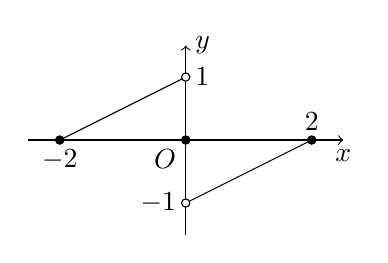
\begin{tikzpicture}
\draw[->](-2,0)--(2,0)node[below]{$x$};
\draw[->](0,-1.2)--(0,1.2)node[right]{$y$};
\draw(-1.6,0)node[below]{$-2$}--(0,0.8)node[right]{1};
\draw(1.6,0)node[above]{2}--(0,-0.8)node[left]{$-1$};
\filldraw[fill=black](0,0)circle(1.5pt)node[below left]{$O$};
\filldraw[fill=black](-1.6,0)circle(1.5pt);
\filldraw[fill=black](1.6,0)circle(1.5pt);
\filldraw[fill=white](0,0.8)circle(1.5pt);
\filldraw[fill=white](0,-0.8)circle(1.5pt);
\end{tikzpicture}
\begin{enumerate}
\item 求$y=f(x)$的解析式; 
\item 若$g(x)=f(\frac{1}{x})$, 求$y=g(x)$的解析式, 并作出$g(x)$的图像. 
\end{enumerate}
\begin{jieda}
\begin{enumerate}
\item $f(x)=\begin{cases}
\frac{1}{2}x+1, & x\in[-2,0)\\
0, & x = 0 \\
\frac{1}{2}x-1, & x\in(0,2]
\end{cases}$. 

\item $g(x)=\begin{cases}
\frac{1}{2x}+1, & x\leq-\frac{1}{2}\\
\frac{1}{2x}-1, & x\geq\frac{1}{2}
\end{cases}$. \\
图像如ggb代码: \verb|if(x<=-0.5,1/(2x)+1,x>=0.5,1/(2x)-1)|
\end{enumerate}
\ps 正确率太低, 问题集中在$g(x)$的定义域上.
\end{jieda}
\begin{vspace_}
\vsp[5]
\end{vspace_}

\item 
\begin{enumerate}
\item 已知$y=f(x)$是一次函数, 且$3f(x+1)-2f(x-1)=2x+17$, 求$f(x)$; 
\item 已知$y=f(x)$是二次函数, 且$f(0)=0$, $f(x+1)=f(x)+x+1$, 求$f(x)$. 
\item 已知函数$y=f(x)$满足$2f(x)+f(\frac{1}{x})=3x$, 则$f(x)$=\blkda{$2x-\dfrac{1}{x}$}. 
\end{enumerate}
\begin{jieda}
待定系数法. 
\begin{enumerate}
\item $f(x)=kx+b$, 则$3f(x+1)-2f(x-1)=3k(x+1)+3b-2k(x-1)-2b=kx+5k+b$. \\
故$k=2\land 5k+b=17$, 即$(k,b)=(2,7)$. 于是$f(x)=2x+7$. 

\item 因为$f(0)=0$, 故设$f(x)=ax^2+bx$, 则$f(x+1)-f(x)=a(x+1)^2+b(x+1)-ax^2-bx=2ax+a+b$. \\
故$2a=1\land a+b=1$, 即$(a,b)=(\frac{1}{2},\frac{1}{2})$. 于是$f(x)=\dfrac{1}{2}x^2+\dfrac{1}{2}x$. 

\item 
$\begin{cases}
2f(x)+f(\frac{1}{x})=3x\\
2f(\frac{1}{x})+f(x)=\frac{3}{x}
\end{cases}$, 解得$f(x)=2x-\dfrac{1}{x}$. 
\end{enumerate}
\end{jieda}

\begin{vspace_}
\vsp[5]
\end{vspace_}

\item 已知函数$y=f(x)$与$y=g(x)$在$[-2,2]$的图像如图所示: \\
\begin{minipage}{\linewidth}
\centering

\includegraphics[totalheight=6\baselineskip]{./bodyxb/src/bx01ch03hanshudeyunsuan02t1401.png}
\qquad\qquad

\includegraphics[totalheight=6\baselineskip]{./bodyxb/src/bx01ch03hanshudeyunsuan02t1402.png}
\end{minipage}

判断下列命题的真假, 并说明理由: 
\begin{enumerate}
\item 方程$f(g(x))=0$有且仅有6个根; 
\item 方程$g(f(x))=0$有且仅有3个根; 
\item 方程$f(f(x))=0$有且仅有5个根; 
\item 方程$g(g(x))=0$有且仅有4个根. 
\end{enumerate}
\begin{jieda}
$f(x)=0$的根可取近似值为$0,\pm1.5$; $g(x)=0$的根可取近似值为$-1.8,0.4$. 
\begin{enumerate}
\item $f(g(x))=0\iff g(x)=0,\pm1.5$, 结合$g(x)$的图像可得解的个数为$3+3=6$个. 
\item $g(f(x))=0\iff f(x)=-1.8,0.4$, 结合$f(x)$的图像可得解的个数为$1+3=4$个. 
\item $f(f(x))=0\iff f(x)=0,\pm1.5$, 结合$f(x)$的图像可得解的个数为$3+2=5$个. 
\item $g(g(x))=0\iff g(x)=-1.8,0.4$, 结合$g(x)$的图像可得解的个数为$2+2=4$个. 
\end{enumerate}
综上, 只有(2)是假命题, 其他都是真命题. 
\end{jieda}

\end{enumerate}

C组：
\begin{enumerate}
    \item 已知$f(x) = |1-2x|, x \in [0, 1]$，求方程$f(f(f(x))) = \dfrac{1}{2}x$的解的个数.
    \begin{jieda}
    本题应将方程的解的个数转化为两个函数的交点的个数。 \\
    首先考虑$f(x)$的图象为一条折线（如下图中的红线），端点为$(0, 1), (1, 1)$和$(\dfrac{1}{2}, 0)$。\\
    那么从$f(x)$变换到$f(f(x))$的过程中，对图象上每一个点固定横坐标，纵坐标变为原来的$-2$倍再向上一个单位，结果如下图蓝线，原本红线中纵坐标为0或1的点（最值点）在变换到蓝线后纵坐标都为1，在原本红线中相邻的两个最值点的中点位置的点会被变换到$x$轴上。 \\
    从$f(f(x))$变换到$f(f(f(x)))$的过程也是一样的规律，由此可以得到下图中的绿线。\\
    而$y = \dfrac{x}{2}$不难绘出，由此可以看到下图中绿线和黑线两者的交点个数为8个。\\
    \begin{minipage}{\linewidth}
\centering

\includegraphics[height=5\baselineskip]{./bodyxb/src/bx01ch03sec4hanshudeyunsuanC1_1.png}\qquad

\includegraphics[height=5\baselineskip]{./bodyxb/src/bx01ch03sec4hanshudeyunsuanC1_2.png}\qquad

\includegraphics[height=5\baselineskip]{./bodyxb/src/bx01ch03sec4hanshudeyunsuanC1_3.png}\qquad

\includegraphics[height=5\baselineskip]{./bodyxb/src/bx01ch03sec4hanshudeyunsuanC1_4.png}
\end{minipage}
    % 错解
    % 令$f(x) = \dfrac{1}{2}x$，解得$x = \dfrac{2}{5}, \dfrac{3}{5}$，因此问题转化为$f(f(x)) = \dfrac{2}{5} \mbox{或} \dfrac{3}{5}$的解的个数。\\
    % 由$f(x)$图象可知，$f(x) = \dfrac{2}{5} \mbox{或} \dfrac{3}{5}$的解的个数为$4$，且这四个根都在$(0, 1)$之间，问题进一步转化为$f(x)$等于$(0, 1)$之间的四个值的解的个数，应有$8$个值。
    \end{jieda}
    
    \begin{vspace_}
    \vsp[5]
    \end{vspace_}
    \item 设函数$g(x) = x^2 - 2, x \in \mathbf{R}$，$f(x) = \left \{ \begin{array}{ll}
        g(x)+x+4 & x < g(x) \\
        g(x) - x & x \geq g(x)
    \end{array} \right.$，求$f(x)$的值域
    \begin{jieda}
    $[-\dfrac{9}{4}, 0] \cup (2, +\infty)$
    \end{jieda}
    
    \begin{vspace_}
    \vsp[5]
    \end{vspace_}
    \item 已知$\triangle ABC$为等边三角形，$AB = 2$，$P, Q$依次是$AC, AB$上的点，且线段$PQ$将$\triangle ABC$分为面积相等的两部分，设$AP = x, AQ = t, PQ = y$
    \begin{enumerate}
        \item 用解析式将$t$表示成$x$的函数
        \item 用解析式将$y$表示成$x$的函数
        \item 求$y$的最大值与最小值
    \end{enumerate}
    \begin{jieda}
    \begin{enumerate}
        \item $\triangle ABC$的面积为$\sqrt{3}$，由正弦定理$\dfrac{1}{2}tx sin\dfrac{\pi}{3} = \dfrac{\sqrt{3}}{2}$，解得$t = \dfrac{2}{x}$，由$x \in (0, 2], t \in (0, 2]$可知函数为：$t = \dfrac{2}{x}, x \in [1, 2]$
        \item 由余弦定理可知$y^2 = t^2 + x^2 - 2txcos\dfrac{\pi}{3}$，$y = \sqrt{x^2 + \dfrac{4}{x^2} - 2}, 1 \leq x \leq 2$
        \item 因为$1 \leq x \leq 4$，由对勾函数性质可知$x^2 = 2$的时候，$y$取最小值$\sqrt{2}$，$x^2 = 1$的时候，$y$取最大值$\sqrt{3}$.
    \end{enumerate}
    \end{jieda}
    
    \begin{vspace_}
    \vsp[5]
    \end{vspace_}
\end{enumerate}


\section{函数的奇偶性(1)}

\zsd 偶函数、奇函数、函数图像的对称性、抽象函数

A组:
\begin{enumerate}
\item 若定义在$[3-a,5]$上的函数$f(x)$为奇函数，则$a=$\blkda{$8$}. 

\begin{jieda}
定义域对称.
\end{jieda}


\item 若$f(x)$是偶函数，则$f(1+\sqrt{2})-f(\frac{1}{1-\sqrt{2}})$=\blkda{$0$}.


\item 函数$y=2m x^2+(m+1)x+2$是偶函数的充分必要条件是\blkda[2]{$m=-1$}
\begin{jieda}
    \begin{enumerate}
        \item 视角1 \\
        当$m = 0$时，原函数为一次函数，不是偶函数\\
        当$m \neq 0$的时候，原函数为二次函数，原函数是偶函数等价于其对称轴为$y$轴，因此有$- \dfrac{m+1}{4m} = 0$，解得$m = -1$
        \item 视角2 \\
         $f_1(x) = 2m x^2 + 2$是偶函数 \\
         $f_2(x) = (m+1)x$是奇函数($m = -1$时是既奇又偶函数) \\
         两者相加是偶函数说明必有$m = -1$
    \end{enumerate}
    \ps 多项式函数是奇函数等价于偶次方的系数为零, 是偶函数等价于奇次方的系数为零. \\
    \ps 容易出现$x = 0$的答案，如果自变量变为常数，没有自变量了就不再是一个函数了。或者也可以认为强行将原本函数改变，新造了函数$y = 2$。
\end{jieda} 

\item 若$f(x)$是定义在$\mathbb{R}$上的奇函数，当$x\leqslant 0$时，$f(x)=2x^2-x$，则$f(1)+f(-1)=$\blkda{0}.
\begin{jieda}
    利用奇函数的性质，和具体的解析式无关。
\end{jieda}

\item 下面四个结论：\ding{172} 偶函数的图像一定与$y$轴相交；\ding{173} 奇函数的图像一定通过原点；\ding{174}偶函数的图像关于$y$对称；\ding{175} 既是奇函数又是偶函数的函数一定是$f(x)=0(x\in \mathbb{R})$，其中正确命题的序号是\blkda{\ding{174} }.



\end{enumerate}


B组:
\begin{enumerate}
\item 若函数$f(x)=\dfrac{x}{(2x+1)(x-a)}$为奇函数, 则$a$=\blkda{$\dfrac{1}{2}$}. 
\begin{jieda}
定义域关于原点对称是函数具有奇偶性的必要条件. 
\end{jieda}

\item 已知$f(x)=ax^2+bx+3a+b$是定义在$[a-1,2a]$上的偶函数, 则$a$=\blkda{$\frac{1}{3}$}, $b$=\blkda{$0$}. 


\item 已知$f(x)=ax^{2021}+bx^3+cx+2$, 若$f(-3)=1$, 则$f(3)$=\blkda{$3$}. 
\begin{jieda}
$f(x)+f(-x)=4$. 
\end{jieda}


\item 若$y=f(x)$是偶函数, 当$-2\leq x<0$时, $f(x)=\sqrt[3]{x}+x$, 则当$0<x\leq 2$时, $f(x)$=\blkda{$-\sqrt[3]{x}-x$}. 
\begin{jieda}
因为$y=f(x)$是偶函数, 故当$0<x\leq 2$时, $f(x)=f(-x)=\sqrt[3]{-x}+(-x)=-\sqrt[3]{x}-x$. (注意$x$的意义)
\end{jieda}

\item 已知$y=f(x)(x\zr)$是奇函数, 若当$x<0$时, $f(x)=x^{\frac{1}{3}}+2^x-1$, 则函数$f(x)$的解析式\\
$f(x)$=\blkda[4]{$\begin{cases}
x^{\frac{1}{3}}+2^x-1, x\leq 0\\
x^{\frac{1}{3}}-2^{-x}+1, x>0
\end{cases}$}. 
\begin{jieda}
当$x>0$时, $f(x)=-f(-x)=-((-x)^{\frac{1}{3}}+2^{-x}-1)=x^{\frac{1}{3}}-2^{-x}+1$. \\
又上述两式当$x=0$时也满足$f(0)=0$.  \\
\ps 求谁从谁切入，利用奇偶性列出等式，此时$-x$的范围在解析式的范围，将$-x$代入已知解析式整理即可。
\end{jieda}


\item 设奇函数$y=f(x)$的定义域为$[-5,5]$, 当$x\in[0,5]$时, $f(x)$的图像如图所示, 则不等式$f(x)<0$的解集是\blkda[3]{$(-2,0)\cup(2,5]$}. \\

\begin{minipage}{\linewidth}
\centering

\includegraphics[totalheight=6\baselineskip]{./bodyxb/src/bx01ch03hanshudejiouxing02t5.png}
\end{minipage}
\begin{jieda}
为了避免画图, 从而有看起来``曲折''的代数过程. \\
当$x\in[0,5]$时, $f(x)<0$的解为$(2,5]$, $f(x)>0$的解为$(0,2)$.  \\
当$x\in[-5,0]$时, $f(x)<0\iff -f(x)>0\iff f(-x)>0\iff -x\in(0,2)\iff x\in(-2,0)$. 
\end{jieda}


\item 函数$y=\sqrt{x-1}+\sqrt{x-1}$\dotfill(\kh{D})
\xx{是奇函数}{是偶函数}{既是奇函数又是偶函数}{是非奇非偶函数}
\begin{jieda}
定义域为$\{1\}$, 故非奇非偶. 
\end{jieda}


\item 下列判断正确的是\dotfill(\kh{D})
\xx{$f(x)=\left(\sqrt{x}\right)^2$是偶函数}
{$f(x)=\dfrac{x^2-x}{x-1}$是奇函数}
{$f(x)=x^2+\dfrac{1}{x^2}(x\in\mathbb{R}^+)是偶函数$}
{$f(x)=\dfrac{2^x+1}{2^x-1}$是奇函数}
\begin{jieda}
A,B,C的定义域皆不关于原点对称. 
\end{jieda}


% 2011广东
\item 设$f(x)$和$g(x)$分别是$\mathbb{R}$上的偶函数和奇函数, 则下列结论恒成立的是\dotfill(\kh{A})
\xx{$f(x)+\abs{g(x)}$是偶函数}{$f(x)-\abs{g(x)}$是奇函数}{$\abs{f(x)}+g(x)$是偶函数}{$\abs{f(x)}-g(x)$是奇函数}
\begin{jieda}
$g(x)$为奇函数，则$|g(x)|$为偶函数，偶函数$+$偶函数还是偶函数，故$A, B$都是偶函数，$A$正确，$B$错误。\\
$f(x)$是偶函数，$|f(x)|$还是偶函数。奇函数$+$偶函数的结果是不确定的（如果两个函数都不是“既是奇函数又是偶函数”的话，结果必然非奇非偶函数）。故$C,D$都错。\\
\ps 任意一个关于定义域关于原点对称的函数都可以写成一个奇函数加上一个偶函数（包含其中之一为既奇又偶的情况）：$h(x) = \dfrac{h(x)+h(-x)}{2} + \dfrac{h(x) - h(-x)}{2}$
\end{jieda}


\item 函数$f(x)=x\abs{x+a}+b$是奇函数的充要条件是\dotfill(\kh{B})
\xx{$ab=0$}{$a^2+b^2=0$}{$a=b$}{$a+b=0$}
\begin{jieda}
奇函数若在$x=0$处有定义, 则此处的函数值为零, 即$f(0)=0$, 于是$b=0$. \\
故$f(x)=x\abs{x+a}$. 于是由$f(x)$为奇函数，不难得到$a=0$, 比如$f(-a)+f(a)=0$. 
\end{jieda}


\item 已知函数$y=f(x)$是$\mathbb{R}$上的不恒为0的函数, 且对于任意的$a,b\zr$, 都有$f(ab)=af(b)+bf(a)$, 则函数$f(x)$\dotfill(\kh{A})
\xx{是奇函数}{是偶函数}{既是奇函数又是偶函数}{既不是奇函数也不是偶函数}
\begin{jieda}
容易判断出应该利用迭代法解决问题，首先考虑带入常值特值。令$a=b=0$, 则$f(0)=0$. 令$a=b=1$, 则$f(1)=0$. 令$a=b=-1$, 则$f(-1)=0$. \\
下一步为了判断奇偶性，应当考虑得到$-x$的形式，故令$a=-1$, $b=x$, 则$f(-x)=-f(x)+xf(-1)=-f(x)$. 故$f(x)$是奇函数. \\
又不恒为0, 故仅是奇函数. 
\end{jieda}


\item 判断下列函数的奇偶性: 
\begin{enumerate}
\item $f(x)=(x-1)\sqrt{\dfrac{1+x}{1-x}}$; 
\item $f(x)=\dfrac{x^3+ax^2}{x+a}$. 
\end{enumerate}
\begin{jieda}
\begin{enumerate}
\item 定义域为$[-1,1)$, 不关于原点对称, 故非奇非偶. 
\item $f(x)=x^2(x\neq -a)$. 当$a=0$时, 易得偶函数; 当$a\neq 0$时, 非奇非偶. 
\end{enumerate}
\end{jieda}
\begin{vspace_}
\vsp[3]
\end{vspace_}


\item 已知$f(x)=\dfrac{ax^2+1}{bx+c}(a,b,c\zz)$为奇函数, 且$f(1)=2$, $f(2)<3$, 求$a,b,c$的值. 
\begin{jieda}
因为$f(x)$是奇函数, 故$f(0)=0$或$f(0)$无意义. (因为不确定$0$是否在定义域中)\\
若$c\neq 0$, 则$f(0)=\dfrac{1}{c}\neq 0$, 故$c=0$, 即$f(x)=\dfrac{ax^2+1}{bx}$. \\
又$\begin{cases}
f(1)=2\\
f(2)<3
\end{cases}$, 
即$\begin{cases}
\frac{a+1}{b}=2\\
\frac{4a+1}{2b}<3
\end{cases}$, 上式得到$a = 2b-1$代入第二个式子消元得到$\dfrac{8b-3}{2b}<3$，即$1 < \dfrac{3}{2b}$，即$b \in (0, \dfrac{3}{2})$. 又因为$b \zz$，因此$b = 1$，进一步得到$a = 1$. \\
综上, $a=b=1, c=0$. 
\end{jieda}
\begin{vspace_}
\vsp[5]
\end{vspace_}

\item 定义两种运算: $a\oplus b=\sqrt{a^2-b^2}$, $a\otimes b=\abs{a-b}$, 
求函数$f(x)=\dfrac{2\oplus x}{(x\otimes 2)-2}$的定义域, 并判断奇偶性. 
\begin{jieda}
$f(x)=\dfrac{\sqrt{4-x^2}}{\abs{x-2}-2}$. 
于是$\begin{cases}
4-x^2\geq 0\\
\abs{x-2}-2\neq 0
\end{cases}$, 解得$x\in[-2,0)\cup(0,2]$. \\
于是对定义域内任意的$x$有$f(x)=\dfrac{\sqrt{4-x^2}}{-x}$,$f(-x)=\dfrac{\sqrt{4-x^2}}{x}$ , 故$f(-x)=-f(x)$. \\
易知$f(1) \neq f(-1)$，故$f(x)$不是偶函数，
所以$y=f(x)$是$[-2,0)\cup(0,2]$上的奇函数. 
\end{jieda}
\begin{vspace_}
\vsp[4]
\end{vspace_}


\item 已知函数$f(x)=x\abs{x+m}+n(m,n\zr)$. 
\begin{enumerate}
\item 求证: $m=n=0$是$f(x)$为奇函数的充要条件; 
\item 若常数$n=-4$, 且$f(x)<0$对任意$x\in[0,1]$恒成立, 求$m$的取值范围. 
\end{enumerate}
\begin{jieda}
\begin{enumerate}
\item 见第8题; 通过个别函数值的关系得到$m=n=0$后, 还得证明此时对任意$x\zr$, 都有$f(-x)=-f(x)$. 
\item $x\abs{x+m}-4<0\iff x\abs{x+m}<4$. \\
显然$x=0$时恒成立, 故只要考虑$x\in(0,1]$. \\
此时有$\abs{x+m}<\dfrac{4}{x}$, 故$-\dfrac{4}{x}<x+m<\dfrac{4}{x}$, 即$-\dfrac{4}{x}-x<m<\dfrac{4}{x}-x$. \\
对$y=\dfrac{4}{x}-x$而言, 其在$(0,1]$上的最小值为$3$($x=1$时取到); \\
对$y=-\dfrac{4}{x}-x$而言, 其在$(0,1]$上的最大值为$-5$($x=1$时取到). \\
综上, $m\in(-5,3)$. \\
\ps 据说只要$f(1)$满足即得答案, 从过程中可以看出, 的确如此. 然而实际上这样来求解, 是错误的. % 20230903
\end{enumerate}
\end{jieda}
\begin{vspace_}
\vsp[5]
\end{vspace_}
\end{enumerate}

C组：
\begin{enumerate}
    \item 若函数$f(x) = \dfrac{(\sqrt{1008}x + \sqrt{1009})^2 + sin2018x}{2016x^2+2018}$的最大值为$M$，最小值为$m$，则$M + m = $\blkda{$1$}.
    \begin{jieda}
    首先考虑化简变形，令$a = \sqrt{1008}, b = \sqrt{1009}$，\\
    $f(x) = \dfrac{(ax+b)^2 + sin(2b^2x)}{2(ax)^2+2b^2} = \dfrac{1}{2} + \dfrac{2abx + sin(2b^2x)}{2(ax)^2+2b^2}$ \\
    $y = 2abx$为奇函数，$y = sin(2b^2x)$为奇函数，故$y = 2abx + sin(2b^2x)$为奇函数；$y = 2(ax)^2+2b^2$为偶函数；故$y = \dfrac{2abx + sin(2b^2x)}{2(ax)^2+2b^2}$为奇函数，故其最大值和最小值之和为0，因此$M + m = 1$
    \end{jieda}
    \item 已知函数$f(x) = x^3 + sinx (x \in \mathbf{R})$，函数$g(x)$满足$g(x)+g(2-x) = 0(x \in \mathbf{R})$，若函数$h(x) = f(x-1)-g(x)$恰有2019个零点，则所有这些零点之和为\blkda{$2019$}.
    \begin{jieda}
    易知$f(x)$为奇函数，故$f(x-1)$关于$(1, 0)$中心对称。又由$g(x)+g(2-x) = 0(x \in \mathbf{R})$可知$g(x)$关于$(1, 0)$中心对称。因此$h(x)$关于$(1, 0)$中心对称，因此其零点必然关于$1$对称（奇数个零点代表有一个零点为1），故所有零点之和为零点个数，2019.
    \end{jieda}
\end{enumerate}


\section{函数的奇偶性(2)}

A组:
\begin{enumerate}
\item 若函数$y=f(x),x\in [-2,a]$是偶函数，则$a$的值为\blkda{2}.

\item 若$f(x),g(x)$都是定义在$[-a,a]$上的奇函数，且$g(x) \neq 0$，则下列函数中，为奇函数的是:\blkda{\ding{172}\ding{174}};为偶函数的是：\blkda{ \ding{173} \ding{175}  }. \\
\ding{172}$f(x)+g(x)$; \ding{173} $f(x)\cdot g(x)$;\ding{174}$f(x)-g(x)$;\ding{175} $\frac{f(x)}{g(x)}$

\item 若$y=f(x) (x\in [-1,1])$，则 $F(x)=f(x)+f(-x)$是\blkda{偶}函数，$G(x)=f(x)+f(-x)$是\blkda{奇}函数. （填奇偶性）

\item 已知$y=f(x)+x^2$是奇函数，且$f(1)=1$，若$g(x)=f(x)+2$，则$g(-1)=$\blkda{$-1$}.

\item 已知对于任意实数$x$，函数$f(x)$满足$f(-x)=f(x)$，若方程$f(x)=0$有$2019$个实数解，则这$2019$个实数解之和为\blkda{0}.

    
\end{enumerate}


B组：
\begin{enumerate}

\item 已知$f(x)=ax^2+(b-3)x+3(x\in[a^2-2,a])$是偶函数, 则$a+b$=\blkda{$4$}.
\begin{jieda}
$a^2-2+a=0\mbox{且} a > a^2 - 2$, 则$a=1$, $b-3=0$(奇次方系数为零). 
\end{jieda}

\item 如果函数$y=x^2+bx+c$是偶函数，则实数$b,c$所满足的一个充要条件是\blkda{$b=0$}.

\item 若函数$y=(x+a)(bx+2a)$（常数$a,b\in \mathbb{R}$）是偶函数，且它的最大值为$4$，则该函数的解析式 $y=$\blkda{$-2x^2+4$}.


\item 已知函数$f(x)=x^5+ax^3+bx-8$, 且$f(-2)=10$, 则$f(2)$=\blkda{$-26$}
\begin{jieda}
$f(x)+f(-x)=-16$
\end{jieda}


\item 已知$y=f(x)(x\zr)$是奇函数, $y=g(x)(x\zr)$是偶函数, 若$y=f(x)+g(x)$的值域为$[-1,4)$, 则$y=f(x)-g(x)$的值域为\blkda{$(-4,1]$}. 
\begin{jieda}
$h(x)=f(x)+g(x)$, 则$h(-x)=f(-x)+g(-x)=-f(x)+g(x)$, 且$y=h(x)$与$y=h(-x)$的值域相同. \\
故$y=-h(-x)$的值域为$(-4,1]$. 
\end{jieda}

\item 已知函数 $y=\left\{\begin{array}{ll}-x^2+x, & x>0 \\ a x^2+x, & x<0\end{array}\right.$ 是奇函数, 则 $a=$ \blkda{$1$}.
\begin{jieda}
    计算$f(1), f(-1)$即可（利用必要条件解决问题）。
\end{jieda}


\item 设函数 $f(x)=\frac{1-x}{1+x}$ ，则下列函数中为奇函数的是\dotfill(\kh{B})
\xx{$f(x-1)-1$}{$f(x-1)+1$}{$f(x+1)-1$}{$f(x+1)+1$}
\begin{jieda}
    原函数的对称中心为$(-1, -1)$，故其向右平移一个单位再向上平移一个单位之后是奇函数，因此选B
\end{jieda}


\item 已知函数$y=f(x)$是定义在实数集$\bR$上的不恒为零的偶函数, 且对任意实数$x$都有$xf(x+1)=(x+1)f(x)$, 则$f\left(\dfrac{5}{2}\right)$的值是\blkda{$0$}.
\begin{jieda}
$f(x) = \dfrac{xf(x+1)}{x+1} = \dfrac{x}{x+1} \cdot \dfrac{x+1}{x+2} \cdot f(x+2) = \dfrac{xf(x+2)}{x+2} = ... = \dfrac{xf(x+k)}{x+k} (k \in \mathbf{Z}, x \neq \mathbf{Z})$，因此取$x = \dfrac{5}{2}, k = -5$，有$f(\dfrac{5}{2}) = \dfrac{\dfrac{5}{2}f(-\dfrac{5}{2})}{-\dfrac{5}{2}} = -f(-\dfrac{5}{2}) = -f(\dfrac{5}{2})$，因此$f(\dfrac{5}{2}) = 0$
\end{jieda}

\item 给出下列关于函数奇偶性的命题:\\
\ding{172} “函数 $y=f(x)$ 的定义域关于原点对称” 是 “函数 $y=f(x)$ 是偶函数或者奇函数” 的必要条件;\\
\ding{173} 如果一个函数的图像是以坐标原点为对称中心的中心对称图形, 那么这个函数是奇函数;\\
\ding{174} 定义在 $\mathbf{R}$ 上的函数 $y=f(x)$ 若满足 $f(-1)=f(1)$, 那么 $y=f(x)$ 是偶函数;\\
\ding{175} 定义在 $\mathbf{R}$ 上的函数 $y=f(x)$ 若满足 $f(-1) \neq-f(1)$, 那么 $y=f(x)$ 不是奇函数;\\
其中真命题的序号是\blkda{\ding{172}\ding{173}\ding{175} }(填所有真命题的序号).


\item 已知函数 $y=f(x)$ 与 $y=g(x)$ 都是定义域为 $\mathbf{R}$ 的奇函数, 且 $g(x)$ 不恒为零,则给 出下列四个函数: \ding{172}  $F(x)=f(x)+g(x)$; \ding{173}  $F(x)=f(x)-g(x)$;\ding{174}  $F(x)=f(x) \cdot g(x)$; \ding{175}  $F(x)=\frac{f(x)}{g(x)}$; 其中一定是偶函数的是\blkda{ \ding{174}\ding{175} }.


\item 已知 $f(x)=\dfrac{a x+b}{1+x^2}$, 若函数 $y=f(x)$ 是定义在 R 上的奇函数, 且 $f\left(\dfrac{1}{2}\right)=\dfrac{2}{5}$.
\begin{enumerate}
    \item 求函数 $y=f(x)$ 的解析式;
    \item 求函数 $y=f(x)$ 的值域.
\end{enumerate}

\begin{jieda}
    \begin{enumerate}
        \item 根据$f(0) = 0$有$b = 0$，$f(x)=\dfrac{ax}{1+x^2}$，代入$f(\dfrac{1}{2}) = \dfrac{2}{5}$，得到$a = 1$，故$f(x)=\dfrac{x}{1+x^2}$；经检验$f(x)=\dfrac{x}{1+x^2}$是奇函数。
        \item \begin{enumerate}
            \item 首先$f(0) = 0$，故$0$在值域中。
            \item 当$x \neq 0$时，$f(x) = \dfrac{1}{x + \dfrac{1}{x}}$，根据对勾函数性质可知$x + \dfrac{1}{x} \in (-\infty, -2] \cup [2, +\infty)$，因此$\dfrac{1}{x + \dfrac{1}{x}} \in [-\dfrac{1}{2}, 0) \cup (0, \dfrac{1}{2}]$
        \end{enumerate}
        综上，$f(x)$的值域为$[-\dfrac{1}{2},\dfrac{1}{2}]$. \\
        \ps  求一次比二次函数的值域，注意分类讨论。
    \end{enumerate}
\end{jieda}
\begin{vspace_}
   \vsp[3] 
\end{vspace_}

\item 已知函数 $f(x)=x^2+\dfrac{a}{x} \quad(x \neq 0$, 常数 $a \in \mathbf{R})$.
\begin{enumerate}
    \item 当 $a=2$ 时, 解不等式 $f(x)-f(x-1)>2 x-1$ ；
    \item 讨论函数 $f(x)$ 的奇偶性,并说明理由.
\end{enumerate}
\begin{jieda}
    \begin{enumerate}
        \item 代入$a = 2$，不等式为$(x^2 + \dfrac{2}{x}) - ((x-1)^2 + \dfrac{2}{x-1}) > 2x-1$，重组整理得$(2x-1) + (\dfrac{2}{x} - \dfrac{2}{x-1}) > 2x-1$，进一步化简有$\dfrac{2}{x} > \dfrac{2}{x-1}$，解得$x \in (0,1)$；
        \item \begin{enumerate}
            \item $a = 0$时，$f(x) = x^2$，为偶函数.
            \item $a \neq 0$时，$f(a) = a^2+1, f(-a) = a^2-1$，两者既不相等也不互为相反数，因此$f(x)$必然是非奇非偶. 
        \end{enumerate}
        \ps 奇函数$+$偶函数的结果是不确定的（如果两个函数都不是“既是奇函数又是偶函数”的话，结果必然非奇非偶函数）
    \end{enumerate}
\end{jieda}
\begin{vspace_}
   \vsp[4] 
\end{vspace_}


\item 
\begin{enumerate}

\item 判断函数$f(x)=ax^2+\dfrac{b}{x}$的奇偶性. 
\begin{jieda}
定义域别忘了. \\
$a=0$时, 奇函数; $b=0$时, 偶函数; $a=b=0$时, 既是奇函数又是偶函数; $ab\neq 0$时, 非奇非偶. 
\end{jieda}


\item 已知函数$f(x)=\dfrac{x+a}{x^2+bx+1}(-1\leq x\leq 1)$为奇函数, 试求$a,b$的值. 
\begin{jieda}
$0\in[-1,1]$, 故$f(0)=0$, 于是易得$a=0$, 则$f(x)=\dfrac{x}{x^2+bx+1}$. 此时不难得到$b=0$. \\
\ps 证明过程略. 
\end{jieda}


\item 已知$f(x)$是偶函数, $g(x)$是奇函数, $f(x)+g(x)=x^2+x-2$, 求$f(x)$与$g(x)$的解析式. 
\begin{jieda}
$f(-x)+g(-x)=(-x)^2+(-x)-2$, 则$f(x)-g(x)=x^2-x-2$, 于是$\begin{cases}
f(x)+g(x)=x^2+x-2\\
f(x)-g(x)=x^2-x-2
\end{cases}$. \\
解得$f(x)=x^2-2$, $g(x)=x$. \\
\ps 第一步若不理解, 那么令$h(x)=f(x)+g(x)$. \\
另外, $f(x)=\dfrac{f(x)+f(-x)}{2}+\dfrac{f(x)-f(-x)}{2}$. ``什么都没变, 却有了不同''. 
\end{jieda}
\end{enumerate}

\begin{vspace_}
   \vsp[5] 
\end{vspace_}


\item 已知函数$y=f(x)$是$\mathbb{R}$上的不恒为0的函数, 且对于任意的$a,b\zr$, 都有$f(ab)=af(b)+bf(a)$；
\begin{enumerate}
    \item 求$f(0), f(1)$的值；
    \item 判断$y=f(x)$的奇偶性，并证明你的结论. 
\end{enumerate}
\begin{jieda}
容易判断出应该利用迭代法解决问题，首先考虑带入常值特值。令$a=b=0$, 则$f(0)=0$. 令$a=b=1$, 则$f(1)=0$. 令$a=1, b=-1$, 则$f(-1)=0$. \\
下一步为了判断奇偶性，应当考虑得到$-x$的形式，故令$a=-1$, $b=x$, 则对任意$x$有$f(-x)=-f(x)+xf(-1)=-f(x)$. 故$f(x)$是奇函数. \\
又不恒为0, 故仅是奇函数. 
\end{jieda}

\begin{vspace_}
   \vsp[5] 
\end{vspace_}

\item 已知$y=f(x)$对任意实数$a,b$都有$f(a+b)=f(a)+f(b)$成立. 
\begin{enumerate}[(1)]
\item 求$f(0)$的值; 
\item 判断函数$y=f(x)$的奇偶性; 
\item 若$f(-3)=a$, 用$a$的代数式表示$f(12)$的值. 
\end{enumerate}
\begin{jieda}
\begin{enumerate}
\item 令$a=b=0$, 则易得$f(0)=0$. 
\item 令$a=x$, $b=-x$, 则$f(0)=f(x)+f(-x)$, 即对任意$x$有$f(-x)=-f(x)$, 故$f(x)$为$\bR$上的奇函数. 
\item $f(kx)=kf(x)(k\zz)$（数学归纳法可证）. \\
$f(12)=f(6)+f(6)=2f(6)=2(f(3)+f(3))=4f(3)=-4f(-3)=-4a$. 
\end{enumerate}
\end{jieda}

\begin{vspace_}
   \vsp[5] 
\end{vspace_}


\item 记函数 $f(x)$ 的定义域为 $D$, 若存在 $x_0 \in D$, 使 $f\left(x_0\right)=x_0$ 成立, 则称 $\left(x_0, y_0\right)$为坐标的点为函数 $f(x)$ 图象上的不动点.
\begin{enumerate}
    \item 若函数 $f(x)=\dfrac{3x+a}{x+b}$ 图象上有两个关于原点对称的不动点, 求 $a, b$ 应满足的条件;
    \item 下述命题：“若定义在 $R$ 上的奇函数 $f(x)$ 图象上存在有限个不动点，则不动点有奇数个” 是否正确? 若正确, 给予证明; 若不正确, 请举一反例.
\end{enumerate}
\begin{jieda}
    \begin{enumerate}
        \item 
        根据题意方程$f(x) = x$应有两个相异的互为相反数的实根，即$x^2 + (b-3)x - a = 0$有两个相异的互为相反数的实根（且不为$-b$）\\
        根据韦达定理有$b-3 = 0$，故$b = 3$. 此时计算判别式有$\Delta = 4a > 0$，故$a > 0$. 又因为$b^2 - a \neq 0$，所以$a \neq 9$.\\
        综上$b = 3, a \in (0, 9) \cup (9, +\infty)$
        \\
        \ps 好想不好说的几何角度：$f(x)=\dfrac{3x+a}{x+b} = 3 + \dfrac{a - 3b}{x+b}$ 为对称中心为$(-b, 3)$的双曲线（$a = 3b$不符合题意），有两条对称轴$y = x + (3+b)$和$y = -x + (3-b)$。当且仅当$b = 3$时，满足题意。随着$b$的改变，双曲线在竖直方向上移动，与$y = x$的交点必然不再满足对称性（只有双曲线沿着$y = -x + (3-b)$的方向移动才可以保持对称性）。故$b = 3, f(x) = 3 + \dfrac{a-9}{x+3}$. 当$a > 9$时双曲线在两区间上都单调减，必然会与$y = x$有两个交点。$a < 9$时双曲线在两支上都单调减，双曲线右下支上的点$(\sqrt{9-a}-3, 3-\sqrt{9-a})$为双曲线与$y = -x$交点，该处的切线与$y = x$平行。随着$a$的减小，$(\sqrt{9-a}-3, 3-\sqrt{9-a})$在沿$y = -x$移动，从$y = x$的左上移动到右下，$(\sqrt{9-a}-3, 3-\sqrt{9-a})$在$y = x$左上时根据函数零点存在定理必然有两交点，而右下则没有，边界情况为$a = 0$，故$a \in (0, 9) \cup (9, +\infty)$
        \item 正确，证明如下：\\
        设$g(x) = f(x) - x$，故$g(x)$的零点即是$f(x)$的不动点的横坐标。易知$g(x)$是奇函数，因此当$g(x)$零点有限的时候，若$g(x_0) = 0$，则$g(-x_0) = 0$。又因为有$g(0) = 0$，因此当$g(x)$零点有限的时候，$g(x)$的零点必为奇数个。 \\
        \ps 根据对称性可知不动点会成对出现，唯一的特例是原点，相当于两个不动点重合了，因此是奇数个。
    \end{enumerate}
\end{jieda}

\begin{vspace_}
   \vsp[5] 
\end{vspace_}
\end{enumerate}

C组：
\begin{enumerate}
    \item 已知$f(x) = \dfrac{(2^x+1)^2}{2^x \cdot x}+1$在$[-2018, -1]\cup[1, 2018]$上最大值为$M$,最小值为$m$,则$M+m = $\blkda{$2$}.
    \begin{jieda}
    设$g(x) = \dfrac{(2^x+1)^2}{2^x \cdot x}$，则$g(x) = \dfrac{2^x+\dfrac{1}{2^x}+2}{x} = \dfrac{2^x+2^{-x}+2}{x}$，故$g(-x) = -g(x)$，即$g(x)$为奇函数，故$M+m = 2$
    \end{jieda}
    \item 函数$y = f(x)$与函数$y = g(x)$有相同的定义域，且都不是常值函数。若对定义域中任意$x$都有$f(x)+f(-x) = 0, g(x)\cdot g(-x) = 1$，且$x \neq 0$时$g(x) \neq 1$. 设$F(x) = \dfrac{2f(x)}{g(x) - 1} + f(x)$的奇偶性并证明.
    \begin{jieda}
        $F(x)$是偶函数。 \\
        根据题意显然有$f(x), g(x)$的定义域关于原点对称，因此$F(x)$的定义域也关于原点对称。\\
        对定义域内任意的$x$都有：\\
        $F(-x) = \dfrac{2f(-x)}{g(-x) - 1} + f(-x) = \dfrac{-2f(x)}{\dfrac{1}{g(x)} - 1} - f(x) = \dfrac{2f(x)g(x)}{g(x)-1} - f(x) \\
        = \dfrac{2f(x)g(x)- f(x)g(x) + f(x)}{g(x)-1} = \dfrac{f(x)g(x) + f(x)}{g(x)-1} = \dfrac{f(x)(g(x) + 1)}{g(x)-1}$ \\
        $F(x) = \dfrac{2f(x)}{g(x) - 1} + f(x) = \dfrac{2f(x) + f(x)g(x) - f(x)}{g(x) - 1} = \dfrac{f(x) + f(x)g(x)}{g(x) - 1} = \dfrac{f(x)(1+g(x))}{g(x) - 1}$ \\
        因此$F(x) = F(-x)$ \\
        又因为$f(x), g(x)$不为常值函数，故$F(x)$不恒为0，因此$F(x)$不是奇函数。因此$F(x)$是偶函数。
    \end{jieda}

\end{enumerate}


\section{函数的单调性(1)}

\zsd 单调性定义、单调区间、抽象函数的单调性


A组：
\begin{enumerate}
\item 函数 $y=\dfrac{k}{x}(k>0)$ 的单调减区间是\blkda[4]{$(-\infty,0)$和$(0,+\infty)$}.

\item 函数 $y=-x^2-2 x+3$ 的单调增区间是\blkda{$(-\infty,-1)$} ；单调减区间是\blkda{$(-1,+\infty)$}.


\item 函数 $f(x)=|x+1|+|x-2|$ 的严格单调减区间是\blkda{$(-\infty,-1)$}.

\item 在区间 $(-\infty, 0)$ 上为严格增函数的是\dotfill(\kh{B})
\xx{$y=1$}
{$y=\frac{x}{1-x}+2$}
{$y=-x^2-2 x-1$}
{$y=1+x^2$}


\item 函数 $y=-\sqrt{x^2}$ 在 $R$ 上\dotfill(\kh{B})
\xx{是严格增函数}
{不是单调函数}
{是严格减函数}
{是常值函数}

\item 若函数 $f(x)=(2 a-1) x+b$ 在 $R$ 上是减函数, 则实数 $a$ 的取值范围为\blkda{$(-\infty,\frac{1}{2}]$}

\item 已知函数$f(x)=\begin{cases}
x^2-4ax+2, & x<1\\
\frac{a}{x}, & x\geq 1
\end{cases}$, 
且$f(x)$在$\bR$上严格减, 则实数$a$的取值范围是\blkda{$[\frac{1}{2},\frac{3}{5}]$}.
\begin{jieda}
$2a\geq 1\land a\geq0\land 1^2-4a\cdot 1+2\geq \dfrac{a}{1}$. \\
\ps 分段函数的单调性: 各段单调, 且在分段点处亦有相应的大小关系. (两段上下移动一下? )
\end{jieda}

    
\end{enumerate}


B组：
\begin{enumerate}
\item 函数 $y=k x+b$ 的单调减区间是 $(-\infty,+\infty)$, 则实数 $k$ 的范围是\blkda{$(-\infty, 0]$}. 

\item 函数$f(x)=x+\dfrac{9}{x}$的严格增区间是\blkda[4]{$(-\infty,-3]$和$[3,+\infty)$}. 
\begin{jieda}
$f(x)=ax+\dfrac{b}{x}$的单调性应该是滚瓜烂熟. \\
\ps 单调区间是区间, 区间的``并''未必是区间. 这里不要``并'', 即使``并''之后仍然单调. 
\end{jieda}


\item 函数$f(x)=x-\dfrac{9}{x}$的严格增区间是\blkda[4]{$(-\infty,0)$和$(0,+\infty)$}. 
\begin{jieda}
和函数的单调性若能直接判断, 那就完结了. 
\end{jieda}


\item 函数$y=-(x-3)\abs{x}$的严格单调增区间是\blkda{$[0,\frac{3}{2}]$}. 
\begin{jieda}
$f(x)=(x-a)\abs{x-b}$的图像如何? 数形相结合之后, 数形皆可作为判断单调区间的方法, 只不过``形'' 最好不要作为证明的唯一依据. \\
\ps 解析式中有部分绝对值，要考虑分类讨论，写成分段函数.\\
\ps 错误率高.
\end{jieda}

\item 若函数$f(x)=x^2+2(a-1)x+2$在$(-\infty,4)$上严格减, 则实数$a$的取值范围是\blkda{$a\leq -3$}. 
\begin{jieda}
``二次函数的单调性''的重要性无以复加. 核心: 开口、对称轴. 
\end{jieda}

\item 若函数$f(x)=\dfrac{ax+1}{x+2}$在$(-\infty,-2)$上是严格增函数, 则实数$a$的取值范围是\blkda{$a>\dfrac{1}{2}$}. 
\begin{jieda}
$f(x)=a+\dfrac{1-2a}{x+2}$, 故$1-2a<0$. \\
\ps 如果对$g(x)=\dfrac{ax+b}{cx+d}(c\neq 0, ad-bc\neq 0)$的性质加以研究, 那么本题可以用$f(-4)<f(-3)$得到结果, 也可以用$f(1)<f(\pi)$得到结果. 不明所以者, 略过此法. 
\end{jieda}

\item 若函数$f(x)=\abs{x+1}+\abs{x-a}$在$[2,+\infty)$上是严格增函数, 则实数$a$的取值范围是\blkda{$a\leq 2$}.
\begin{jieda}
心中有图, 结果若出. 
\end{jieda}

% 2004年上海理10
\item 若函数$f(x)=a\abs{x-b}+2$在$[0,+\infty)$上是严格增函数, 则$a,b$的取值范围是\blkda[3]{$a>0,b\leq 0$}. 
\begin{jieda}
比拟二次函数. 
\end{jieda}


\item 若函数$f(x)$在区间$[a,b]$和$(b,c]$上是严格减函数, 则函数$f(x)$在区间$[a,c]$上\dotfill(\kh{D})
\xx{是严格增函数}{是严格增函数, 或严格减函数}{是严格减函数}{未必具有单调性的函数}
\begin{jieda}
把两段图像``随意''地上下移动一下? 再移动一下? 
\end{jieda}

\item 已知函数 $f(x)=|2 x-a|$ 在 $(-\infty, 3)$ 上单调减, 则实数 $a$ 的取值范围是\blkda{$[6,+\infty)$}.
\begin{jieda}
因为 $f(x)=|2 x-a|=\left\{\begin{array}{l}2 x-a, x \geq \frac{a}{2} \\ a-2 x, x<\frac{a}{2}\end{array}\right.$,
所以 $f(x)$ 在 $\left(\frac{a}{2},+\infty\right)$ 上单调增, 在 $\left(-\infty, \frac{a}{2}\right)$ 上单调减,
又函数 $f(x)$ 在 $(-\infty, 3)$ 上单调减，所以 $\frac{a}{2} \geq 3$ ，解得 $a \geq 6$ ，
即实数 $a$ 的取值范围是 $[6,+\infty)$.
故答案为: $[6,+\infty)$
\end{jieda}

\item 已知函数 $f(x)=\left\{\begin{array}{l}x^{2}+2 a x, x \geq-1 \\ (2-a) x+2 a-5, x<-1\end{array}\right.$, 若 $f(x)$ 在 $\mathbf{R}$ 上是严格增函数, 则实数 $a$ 的取值范围是\blkda{$1 \leq a \leq \frac{8}{5}$} .
\begin{jieda}
由函数 $f(x)=\left\{\begin{array}{l}x^{2}+2 a x, x \geq-1 \\ (2-a) x+2 a-5, x<-1\end{array}\right.$ 在 $\mathbf{R}$ 上是严格增函数, 得 $\left\{\begin{array}{l}-a \leq-1 \\ 2-a>0 \\ 1-2 a \geq-(2-a)+2 a-5\end{array}\right.$,解得 $1 \leq a \leq \frac{8}{5}$,
所以实数 $a$ 的取值范围是 $1 \leq a \leq \frac{8}{5}$.
故答案为: $1 \leq a \leq \frac{8}{5}$
\end{jieda}


\item 已知 $x>0, y>0$ ，若 $\sqrt{4 x^{2}+3 x y+y^{2}}+m \sqrt{x y}>2 x+y$ 恒成立，则实数 $m$ 的取值范围是\blkda[3]{$(2 \sqrt{2}-\sqrt{7},+\infty)$}.
\begin{jieda}
原不等式等价于 $m>\frac{2 x+y-\sqrt{4 x^{2}+3 x y+y^{2}}}{\sqrt{x y}}$,令 $z=\frac{2 x+y-\sqrt{4 x^{2}+3 x y+y^{2}}}{\sqrt{x y}}=2 \sqrt{\frac{x}{y}}+\sqrt{\frac{y}{x}}-\sqrt{4 \frac{x}{y}+\frac{y}{x}+3}$.令 $t=2 \sqrt{\frac{x}{y}}+\sqrt{\frac{y}{x}}$, 且 $t \geq 2 \sqrt{2}$,则 $z=t-\sqrt{t^{2}-1}=\frac{1}{t+\sqrt{t^{2}-1}}$ 在 $(2 \sqrt{2},+\infty)$ 上单调减, $\therefore z \leq \frac{1}{2 \sqrt{2}+\sqrt{7}}=2 \sqrt{2}-\sqrt{7}, \therefore m>2 \sqrt{2}-\sqrt{7}$.
故 $m$ 的范围是 $(2 \sqrt{2}-\sqrt{7},+\infty)$.
故答案为: $(2 \sqrt{2}-\sqrt{7},+\infty)$
\end{jieda}

\item 求证: 函数$f(x)=\dfrac{x}{x^2-1}$，$x\in(-1,1)$是严格减函数. 
\begin{jieda}
$f(x_2)-f(x_1)=-\dfrac{(x_2-x_1)(1+x_1x_2)}{(x_1^2-1)(x_2^2-1)}$. 
\end{jieda}
\begin{vspace_}
   \vsp[2] 
\end{vspace_}

\item 求证: 函数$f(x)=x+\dfrac{16}{x}$在区间$(0,4]$上是严格减函数, 在区间$[4,+\infty)$上是严格增函数. 
\begin{jieda}
$f(x_2)-f(x_1)=(x_2-x_1)\cdot\dfrac{x_1x_2-16}{x_1x_2}$. 
\end{jieda}
\begin{vspace_}
   \vsp[2] 
\end{vspace_}


\item 求证: 函数$f(x)=x^3+x$在$\bR$上是严格增函数. 
\begin{jieda}
$f(x_2)-f(x_1)=(x_2-x_1)(x_1^2+x_1x_2+x_2^2+1)$. 
\end{jieda}
\begin{vspace_}
   \vsp[2] 
\end{vspace_}


\item 若函数$f(x)=ax^2-2x-1$在$(-\infty,1)$上是严格减函数, 求实数$a$的取值范围. % \da $a\in[0,1]$
\begin{jieda}
\ps 此类含参问题, 从正面解决的一般方式是先求出与参数相关的结果(这里是单调区间), 然后将这个结果代入条件(这里是包含关系), 解得. 
\end{jieda}
\begin{vspace_}
   \vsp[2] 
\end{vspace_}

\item 已知函数$f(x)=2x-\dfrac{a}{x}, x\in(0,1]$是严格减函数, 求实数$a$的取值范围. 
\begin{jieda}
设$0<x_1<x_2\leq 1$, 则$f(x_2)-f(x_1)=(x_2-x_1)\cdot\dfrac{2x_1x_2+a}{x_1x_2}<0$恒成立. \\
于是$a<-2x_1x_2$恒成立. \\
因为$0<x_1<x_2\leq 1$, 则$-2x_1x_2\in(-2,0)$, 故$a\leq -2$. \\
\ps 对$a$分类讨论是一种解法, 这里写一个运用定义的解法, 关键在于恒成立与等号能否成立. 
\end{jieda}
\begin{vspace_}
   \vsp[3] 
\end{vspace_}


\item 设函数$f(x)=\sqrt{x^2+1}-ax(a>0)$. 
\begin{enumerate}[(1)]
\item 当$a=2$时，判断函数$f(x)$在区间$[0,+\infty)$上的单调性，并证明你的结论.
\item 当$a=\dfrac{1}{2}$时, 证明:函数$f(x)$不是单调函数; 
\item 求实数$a$的取值范围, 使得函数$f(x)$在$[0,+\infty)$上是单调函数. 
\end{enumerate}
\begin{jieda}
\begin{enumerate}[(1)]
\item 略
\item $f(0)=1,f(a)=\sqrt{a^2+1}-a^2$, $f(\sqrt{3})=2-a>1$. \\
\ps $a\in(0,1)$时, $f(2a)=\sqrt{4a^2+1}-2a^2$, 基本上可得$f(0)>f(a)<f(2a)$. 
\item $a\geq 1$. 
\end{enumerate}
\end{jieda}
\begin{vspace_}
   \vsp[4] 
\end{vspace_}

\item 已知 $y=f(x)$ 是定义在 $R$ 上的减函数, 且 $f(x+y)=f(x) \cdot f(y), f(2)=\frac{1}{9}$.
\begin{enumerate}
    \item  求 $f(1) , f(3)$ 的值;
    \item 解不等式: $f(x) \cdot f\left(3 x^2-1\right)<\dfrac{1}{27}$.
\end{enumerate}
\begin{jieda}
    \begin{enumerate}
        \item $f(2) = f(1) \cdot f(1), f(1) = \pm \dfrac{1}{3}$，又因为$f(x)$为减函数，所以$f(1) = \dfrac{1}{3}$ \\ 
        $f(3) = f(1) \cdot f(2) = \dfrac{1}{27}$
        \item $f(x) \cdot f\left(3 x^2-1\right) = f(x+(3x^2-1)) $ \\
        $\dfrac{1}{27} = f(3)$，由于$f(x)$单调减，所以$3x^2 + x - 1 > 3$ 解得$x \in (-\infty, -\dfrac{4}{3}) \cup (1, +\infty)$
    \end{enumerate}
\end{jieda}
\begin{vspace_}
   \vsp[3] 
\end{vspace_}


\item 已知定义在$\bR$上的奇函数$f(x)$在$[0,+\infty)$上是严格增函数, 是否存在实数$m$, 使得$f(4m-2mx)>f(4-2x^2)$
对任意$x\in(0,1)$都成立? 若存在, 求出所以符合条件的实数$m$; 若不存在, 说明理由. 
\begin{jieda}
奇函数$f(x)$在$[0,+\infty)$上是严格增函数, 故$f(x)$在$\bR$上严格单调增. \\
于是$f(4m-2mx)>f(4-2x^2)\iff 4m-2mx>4-2x^2\iff m(2-x)>2-x^2$. \\
因为$x\in(0,1)$, 故$m>\dfrac{2-x^2}{2-x}$. \\
而$y=\dfrac{2-x^2}{2-x}=-(2-x)-\dfrac{2}{2-x}+4$, 故$y_{\max}=4-2\sqrt{2}(x=2-\sqrt{2})$. \\
所以$m>4-2\sqrt{2}$. 
\end{jieda}
\begin{vspace_}
   \vsp[4] 
\end{vspace_}



\item 定义在 $[-1,1]$ 上的奇函数 $f(x)$ 满足 $f(1)=2$, 且当 $a, b \in[-1,1], a+b \neq 0$ 时,有 $\dfrac{f(a)+f(b)}{a+b}>0$.
\begin{enumerate}
    \item 判定函数 $f(x)$ 在 $[-1,1]$ 的单调性并加以证明;
    \item 若 $\dfrac{1}{2} f(x) \leq m^2+2 a m+1$ 对所有 $x \in[-1,1], a \in[-1,1]$ 恒成立, 求 $m$ 的取值范围.
\end{enumerate}
\begin{jieda}
    \begin{enumerate}
        \item 将$\dfrac{f(a)+f(b)}{a+b}>0$中的$b$代换为$-b$有$\dfrac{f(a)+f(-b)}{a-b}>0$，根据$f(x)$是奇函数，可以转化为$\dfrac{f(a)-f(b)}{a-b}>0$，由此可以判断出$f(x)$在$[-1, 1]$上单调增。 \\
        证明略.
        \item 不等式左侧的最大值要小于右侧，因为$f(x)$单调增，所以不等式左侧最大值为$\dfrac{1}{2}f(1) = 1$，由此不等式转化为$0 \leq m^2 + 2am$在$a \in [-1, 1]$恒成立。设$g(a) = 2ma+m^2$，故应有$g(-1) \geq 0, g(1) \geq 0$，因此$m \in (-\infty, -2] \cup [2, +\infty) \cup \{0\}$
    \end{enumerate}
\end{jieda}
\begin{vspace_}
   \vsp[4] 
\end{vspace_}

\end{enumerate}

C组：
\begin{enumerate}
    \item 定义在$(-1, 1)$上的函数$f(x)$满足$f(x) - f(y) = f(\dfrac{x-y}{1-xy}), x \in (-1, 0)$时$f(x) < 0$，若$a = f(\dfrac{3}{7}) + f(\dfrac{1}{3}), b = f(\dfrac{5}{7}), c = f(0)$，则三个实数$a, b, c$从小到大排列的顺序为\blkda{$c < a < b$}
    \begin{jieda}
        首先考虑通过互换$x, y$，得到$f(y) - f(x) = f(\dfrac{y-x}{1-xy})$，与原式联立可得$f(\dfrac{y-x}{1-xy}) = -f(\dfrac{x-y}{1-xy})$。由此可以判断出$f(x)$为奇函数. \\
        令$-1 < x < y < 0$，有$x - y < 0, 1-xy > 0$，故$\dfrac{x - y}{1-xy} < 0$。又因为$x < 0$时$f(x) < 0$因此$f(x) - f(y) < 0$，因此$f(x)$在$(-1, 0)$上单调增，根据奇偶性有$f(x)$在$(-1, 1)$单调增。\\
        考虑令$x = \dfrac{3}{7}, y = -\dfrac{1}{3}$，故$a = f(\dfrac{3}{7}) + f(\dfrac{1}{3}) = f(\dfrac{3}{7}) - f(-\dfrac{1}{3}) = f(\dfrac{\dfrac{3}{7} + \dfrac{1}{3}}{1 + \dfrac{3}{7}\cdot\dfrac{1}{3}}) = f(\dfrac{2}{3})$ \\
        故由单调性可以判断出$c < a < b$
    \end{jieda}
    \begin{vspace_}
       \vsp[4] 
    \end{vspace_}
    \item 已知函数$f(x) = x + \dfrac{m}{x} (m > 0), x \in [\dfrac{1}{2}, 1]$，在函数$f(x)$的值域上任取三个数，都存在以这三个数为边长的三角形，求实数$m$的取值范围。
    \begin{jieda}
        题干条件在函数$f(x)$的值域上任取三个数，都存在以这三个数为边长的三角形即函数值域的上限小于其值域下限的两倍
        易知$y = x + \dfrac{m}{x}$在$x = \sqrt{m}$处取得最小值，因此
        \begin{enumerate}
            \item 若$m < \dfrac{1}{4}$，则$f(x)$在$[\dfrac{1}{2}, 1]$单调增，其值域为$[f(\dfrac{1}{2}), f(1)]$，即$[2m+\dfrac{1}{2}, m+1]$.经检验满足要求
            \item 若$m > 1$，则$f(x)$在$[\dfrac{1}{2}, 1]$单调减，其值域为$[f(1), f(\dfrac{1}{2})]$，即$[m+1, 2m+\dfrac{1}{2}]$.经检验满足要求
            \item 若$m \in [\dfrac{1}{4}, \dfrac{1}{2}]$，$f(x)$在$[\dfrac{1}{2}, 1]$先减后增，其值域为$[f(\sqrt{m}), f(1)]$，即$[2\sqrt{m}, m+1]$.经检验满足要求
            \item 若$m \in [\dfrac{1}{2}, 1]$，$f(x)$在$[\dfrac{1}{2}, 1]$先减后增，其值域为$[f(\sqrt{m}), f(\dfrac{1}{2})]$，即$[2\sqrt{m}, 2m+\dfrac{1}{2}]$.经检验满足要求
        \end{enumerate}
        综上，$m \in (0, +\infty)$
    \end{jieda}
\end{enumerate}


\section{函数的单调性(2)}
\zsd 复合函数单调性、单调性的应用 \\

A组：
\begin{enumerate}
\item 若奇函数$y=f(x)$在$(0,+\infty)$上为减函数, 则$f(1.4)$、$-f(-\sqrt{2})$、$f(1.5)$的大小关系\\
是\blkda[5]{$f(1.4)\geq-f(-\sqrt{2})\geq f(1.5)$}. 

\item 当$x<0$时, 偶函数$y=f(x)$是严格增函数, 若$x_1<0,x_2>0$, 且$\abs{x_1}<\abs{x_2}$, 则$f(-x_1)$\blkda[1]{$>$}$f(-x_2)$. 
\begin{jieda}
将``自变量''至于同一个单调区间, 然后借助于单调性, ``成功''地``扔掉'' $f$. 
\end{jieda}

\item 定义在$\bR$上的偶函数$f(x)$满足: 对任意的$x_1,x_2\in[0,+\infty)$, $x_1\neq x_2$, 有$\dfrac{f(x_2)-f(x_1)}{x_2-x_1}<0$, 则\dotfill(\kh{A})
\xx{$f(3)<f(-2)<f(1)$}{$f(1)<f(-2)<f(3)$}{$f(-2)<f(1)<f(3)$}{$f(3)<f(1)<f(-2)$}
\begin{jieda}
等价定义: 
\begin{itemize}
\item 严格单调增: $\dfrac{f(x_2)-f(x_1)}{x_2-x_1}>0(x_1\neq x_2)$; 
\item 严格单调减: $\dfrac{f(x_2)-f(x_1)}{x_2-x_1}<0(x_1\neq x_2)$. 
\end{itemize}
\end{jieda}


\item 设$f(x), g(x)$都是单调函数, 则如下四个命题中, 真命题的序号是\blkda{\ding{172},\ding{173}}: 
\begin{dingautolist}{172}
\item 若$f(x)$是严格增函数, $g(x)$是严格增函数, 则$f(x)+g(x)$是严格增函数; 
\item 若$f(x)$是严格增函数, $g(x)$是严格减函数, 则$f(x)-g(x)$是严格增函数; 
\item 若$f(x)$是严格增函数, $g(x)$是严格增函数, 则$f(x)\cdot g(x)$是严格增函数; 
\item 若$f(x)$是严格增函数, $g(x)$是严格减函数, 则$\frac{f(x)}{g(x)}$是严格减函数. 
\end{dingautolist}

\item 已知函数 $f(x)$ 对于任意的 $x_1, x_2 \in(0,+\infty)\left(x_1 \neq x_2\right)$, 都有 $\frac{f\left(x_1\right)-f\left(x_2\right)}{x_1-x_2}<0$, 则 $f(2), f(\pi), f(3)$ 的大小关系为\blkda[4]{$f(\pi)<f(3)<f(2)$ }.
\begin{jieda}
因为函数 $f(x)$ 对于任意的 $x_{1}, x_{2} \in(0,+\infty)\left(x_{1} \neq x_{2}\right)$, 都有 $\frac{f\left(x_{1}\right)-f\left(x_{2}\right)}{x_{1}-x_{2}}<0$,所以 $f(x)$ 在区间 $(0,+\infty)$ 上是减函数,所以 $\pi>3>2$, 所以 $f(\pi)<f(3)<f(2)$.
故答案为: $f(\pi)<f(3)<f(2)$ (或 $f(2)>f(3)>f(\pi)$ ).
\end{jieda}


\item 函数 $f(x)=\frac{1}{\sqrt{x^2-8 x+15}}$ 的单调减区间是\blkda{$(5,+\infty)$}.

\item 设函数 $f(x)=\sqrt{-x^2+5 x+6}$.
\begin{enumerate}
    \item 求 $f(x)$ 的定义域;
    \item 求 $f(x)$ 的单调区间;
    \item 求 $f(x)$ 在区间 $[1,5]$ 的最大值和最小值.
\end{enumerate}
\begin{jieda}
\begin{enumerate}
    \item $[-1,6]$
    \item $f(x)$ 的单调增区间是 $\left[-1, \frac{5}{2}\right]$ ；单调减区间是 $\left[\frac{5}{2}, 6\right]$
    \item $\dfrac{7}{2} ; \sqrt{6}$
\end{enumerate}
\end{jieda}


\end{enumerate}


B组：
\begin{enumerate}
\item 已知函数 $y=f(x)$ 在 $\mathbf{R}$ 上严格单调减，则函数 $y=f(x+2)$ 的单调减区间是\blkda{$[-2,+\infty)$}.


\item 函数 $f(x)$ 在 $\mathbf{R}$ 上严格单调增, $f[f(x)-3 x]=2$, 则 $f\left(\frac{3}{2}\right)=$ \blkda{$5$}.
\begin{jieda}
因为函数 $f(x)$ 在 $\mathbf{R}$ 上单调增, 则存在唯一的实数 $t$, 使得 $f(t)=2$,
又因为 $f[f(x)-3 x]=2$, 则 $f(x)-3 x=t$, 即 $f(x)=3 x+t$,
所以, $f(t)=4 t=2$, 解得 $t=\frac{1}{2}$, 所以, $f(x)=3 x+t$, 故 $f\left(\frac{3}{2}\right)=3 \times \frac{3}{2}+\frac{1}{2}=5$.
故答案为: 5 。
\end{jieda}

\item 若$f(x)$是$\bR$上的严格减函数, 且函数$f(x)$的图像经过点$A(0,1)$和$B(3,-1)$, 则不等式$\abs{f(x+1)}<1$的解集为\blkda{$(-1,2)$}. 
\begin{jieda}
$\abs{f(x+1)}<1\iff -1<f(x+1)<1\iff f(3)<f(x+1)<f(0)\iff 3>x+1>0\iff 2>x>-1$. 
\end{jieda}

\item 已知$f(x)$是定义在$\bR$上的奇函数, 当$x\geq 0$时, $f(x)=x^2+2x$. 若$f(2-a^2)>f(a)$, 则实数$a$的取值范围是\blkda{$(-2,1)$}. 
\begin{jieda}
显然$f(x)$在$[0,+\infty)$上严格单调增, 故$f(x)$在$(-\infty,0]$上严格单调增, 于是$f(x)$在$\bR$上严格单调增. \\
所以$f(2-a^2)>f(a)\iff 2-a^2>a$. 
\end{jieda}


\item 已知奇函数$f(x)$在$(-\infty,0)$上是严格减函数, $f(2)=0$, 则不等式$(x-1)f(x+1)>0$的解集为\blkda{$(-3,-1)$}.
\begin{jieda}
(不)显然$f(t)>0\iff t\in(-\infty,-2)\cup(0,2)$, $f(t)<0\iff t\in(-2,0)\cup(2,+\infty)$. \\
于是不等式$(x-1)f(x+1)>0$等价于\\
(1) $\begin{cases}
x-1>0\\
f(x+1)>0
\end{cases}$ 或
(2) $\begin{cases}
x-1<0\\
f(x+1)<0
\end{cases}$, \\
即(1)$\begin{cases}
x-1>0\\
x+1\in(-\infty,-2)\cup(0,2)
\end{cases}$ 或
(2) $\begin{cases}
x-1<0\\
x+1\in(-2,0)\cup(2,+\infty)
\end{cases}$. \\
解得$x\in(-3,-1)$. \\
\ps 画个草图就方便很多, 尤其是一开始的``(不)显然''的结果. 
\end{jieda}


\item 已知 $f(x)$ 是定义在区间 $(0,+\infty)$ 上的增函数, 且 $f\left(\frac{x}{y}\right)=f(x)-f(y), f(2)=1$, 如果 $x$ 满足 $f(x)-f\left(\frac{1}{x-3}\right) \leq 2$, 则 $x$ 的取值范围为\blkda{$(3,4]$}.
\begin{jieda}
令 $x=4, y=2$, 则 $f(2)=f(4)-f(2)$, 则 $f(4)=2$,
由 $f(x)-f\left(\frac{1}{x-3}\right) \leq 2$ 可得: $f(x(x-3)) \leq f(4)$,
因为 $f(x)$ 是定义在区间 $(0,+\infty)$ 上的增函数,
所以 $\left\{\begin{array}{l}x>0 \\ \frac{1}{x-3}>0 \\ x(x-3) \leq 4\end{array}\right.$, 解得: $3<x \leq 4$.
则 $x$ 的取值范围为: $(3,4]$ 。
故答案为: $(3,4]$.
\end{jieda}


\item 定义在 $(0,+\infty)$ 上的函数 $f(x)$ 满足 $\frac{x_{2} f\left(x_{1}\right)-x_{1} f\left(x_{2}\right)}{x_{1}-x_{2}}<0$, 且 $f(3)=9$, 则使 $f(x)>3 x$ 成立的 $x$ 的取值范围是\blkda{$(0,3)$} .
\begin{jieda}
由 $\frac{x_{2} f\left(x_{1}\right)-x_{1} f\left(x_{2}\right)}{x_{1}-x_{2}}<0$, 且 $x_{1}, x_{2} \in(0,+\infty)$, 则两边同时除以 $x_{1} x_{2}$ 可得 $\frac{\frac{f\left(x_{1}\right)}{x_{1}}-\frac{f\left(x_{2}\right)}{x_{2}}}{x_{1}-x_{2}}<0$,
令 $g(x)=\frac{f(x)}{x}$, 则原不等式为 $\frac{g\left(x_{1}\right)-g\left(x_{2}\right)}{x_{1}-x_{2}}<0$, 因此函数 $g(x)$ 在 $(0,+\infty)$ 上单调减,由 $f(x)>3 x$, 得 $\frac{f(x)}{x}>3$, 又 $g(3)=\frac{f(3)}{3}=3$, 于是 $g(x)>g(3)$, 解得 $0<x<3$,所以使 $f(x)>3 x$ 成立的 $x$ 的取值范围是 $(0,3)$.
\end{jieda}


\item 已知函数 $f(x)=\left\{\begin{array}{l}x^{2}-a, x \geq 0 \\ 0, x<0\end{array}\right.$, 则满足 $f(a)>f\left(-\frac{a}{3}+\frac{1}{6}\right)$ 的 $a$ 的取值范围是\blkda[4]{$\left(\frac{1}{8}, \frac{1}{2}\right] \cup(1,+\infty)$}.
\begin{jieda}
当 $a<0$ 时, $f(a)=0,-\frac{a}{3}+\frac{1}{6}>0, f\left(-\frac{a}{3}+\frac{1}{6}\right)>0$, 原不等式显然不成立.\\
当 $a=0$ 时, $f(0)=0$, 原不等式不成立.\\
当 $a>0$ 时, 要使得 $f(a)>f\left(-\frac{a}{3}+\frac{1}{6}\right)$, 有两种情况:
第一种情况, 当 $-\frac{a}{3}+\frac{1}{6} \geq 0$ 时, $f(x)$ 在 $[0,+\infty)$ 上单调增, 可得 $a>-\frac{a}{3}+\frac{1}{6} \geq 0$, 解得 $\frac{1}{8}<a \leq \frac{1}{2} ;$\\
第二种情况，当 $-\frac{a}{3}+\frac{1}{6}<0$ 时，则 $f(a)=a^{2}-a=a(a-1)>0$ ，解得 $a>1$ 。\\
综上, $a$ 的取值范围是 $\left(\frac{1}{8}, \frac{1}{2}\right] \cup(1,+\infty)$.\\
故答案为: $\left(\frac{1}{8}, \frac{1}{2}\right] \cup(1,+\infty)$.
\end{jieda}

\item 设$f(x)$是定义在$\bR$上的函数, 且在$\bR$上是严格增函数, 若$F(x)=f(x)-f(-x)$, 则$F(x)$一定是\dotfill(\kh{A})
\xx{奇函数, 且在$\bR$上是严格增函数}{奇函数, 且在$\bR$上是严格减函数}{偶函数, 且在$\bR$上是严格增函数}{偶函数, 且在$\bR$上是严格减函数}



\item 已知 $f(x)$ 是 $\mathbf{R}$ 上的增函数, 若令 $F(x)=f(1-x)-f(1+x)$, 则 $F(x)$ 是 $\mathbf{R}$ 上的\dotfill(\kh{B})
\xx{增函数}{减函数}{先减后增的函数}{先增后减的函数}


\item 已知函数 $f(x)=\frac{\sqrt{2021-a x}}{a-1}$ 在 $[0,1]$ 上严格单调减，那么实数 $a$ 的取值的范围是\blkda[3]{$(-\infty, 0) \cup(1,2021]$}.
\begin{jieda}
当 $a<0$ 时, $y=\sqrt{2021-a x}$ 在 $[0,1]$ 上单调增, 且 $a-1<0$,所以 $f(x)$ 在 $[0,1]$ 上单调减, 符合题意,\\
当 $a=0$ 时, $f(x)=-\sqrt{2021}$ 无单调性, 不符合题意,\\
当 $0<a<1$ 时, $y=\sqrt{2021-a x}$ 在 $[0,1]$ 上单调减, 且 $a-1<0$, 不符合题意,\\
当 $a>1$ 时, $y=\sqrt{2021-a x}$ 在 $[0,1]$ 上单调减, $a-1>0$, 符合题意,\\
还需 $\left\{\begin{array}{l}2021-0 \times a \geq 0 \\ 2021-1 \times a \geq 0\end{array}\right.$ ，解得 $1<a \leq 2021 ，$\\
综上实数 $a$ 的取值的范围是 $(-\infty, 0) \cup(1,2021]$.
\end{jieda}

\item 任意 $t \in \mathrm{R}^{+}$时, $f\left[f(t)-\frac{1}{t}\right]=2$ 恒成立, 且函数 $y=f(t)$ 严格单调, 则 $f\left(\frac{1}{2019}\right)=$ \blkda{$2020$}.
\begin{jieda}
依题意, 令 $f(t)-\frac{1}{t}=m$, 则 $f(t)=m+\frac{1}{t}$, 且 $f(m)=2$,
由函数 $y=f(t)$ 单调，得 $m$ 为正常数，于是 $f(m)=m+\frac{1}{m}=2$ ，解得 $m=1$ ，
因此 $f(t)=1+\frac{1}{t}$, 所以 $f\left(\frac{1}{2019}\right)=1+2019=2020$ 。
故答案为: 2020.
\end{jieda}


\item 已知函数$f(x)$是定义在$(-1,1)$上的奇函数, 且严格单调减. 若$f(1-a)+f(1-a^2)<0$, 则实数$a$的取值范围是\blkda{$(0,1)$}. 
\begin{jieda}
$f(1-a)+f(1-a^2)<0\iff f(1-a)<-f(1-a^2)=f(a^2-1)$. \\
于是$1>1-a>a^2-1>-1$, 解得$a\in(0,1)$. 
\end{jieda}



% 2018届EFZ高三校本10
\item 已知函数$f(x)=\begin{cases}
-x^2+ax, & x\leq 1\\
ax-1, & x>1
\end{cases}$, 
若存在$x_1,x_2\zr$, $x_1\neq x_2$, 使得$f(x_1)=f(x_2)$成立, 则实数$a$的取值范围是\blkda{$a<2$}. 
\begin{jieda}
``若存在$x_1,x_2\zr$, $x_1\neq x_2$, 使得$f(x_1)=f(x_2)$成立''意指``存在水平线与函数图像至少有两个交点''. 
于是(1) 两段中至少有一段中成立; (2) 两段皆单值, 但合在一起时有. \\
若$x\leq 1$时, 成立, 则$\dfrac{a}{2}<1$, 即$a<2$; \\
若$x>1$时, 成立, 则$a=0$; \\
又$f(x)$在$x=1$处是连续的, 故第二种情形是不成立的, 这是因为若$x\leq 1$单调, 则严格单调增, 此时$a\geq 2$; 故$x>1$时, 也是严格单调增. 于是$f(x)$在$\bR$上严格单调增. \\
综上, $a<2$. 
% 易知$y=-x^2+ax$在$-\infty$方向上单调增, 故问题的反面: $f(x)$在$\mathbb{R}$上严格单调增.\\
% 于是$\begin{cases}
% a>0\\
% \dfrac{a}{2}\geq 1\\
% -1+a\leq a-1\\
% \end{cases}$, 
% 解得$a\geq 2$. \\
% 故原题的答案为$a<2$. \\
% \ps 这里的解法其实并不严谨. 
\end{jieda}


\item 已知函数 $f(x)=x^{2}+\frac{2}{x}$.
\begin{enumerate}
    \item 判断 $f(x)$ 在 $(0,1]$ 上的单调性, 并用定义加以证明;
    \item 设函数 $g(x)=\frac{x^{2}}{x^{2}+2 x+1}+\frac{2}{x}+3, x \geq 1$, 求 $g(x)$ 的值域.
\end{enumerate}
\begin{jieda}
\begin{enumerate}
    \item $f(x)$ 在 $(0,1]$ 上的单调减, 证明如下:设 $0<x_{1}<x_{2} \leq 1$, 则 $f\left(x_{1}\right)-f\left(x_{2}\right)=x_{1}^{2}+\frac{2}{x_{1}}-x_{2}^{2}-\frac{2}{x_{2}}$
    $=\left(x_{1}+x_{2}\right)\left(x_{1}-x_{2}\right)+\left(\frac{2}{x_{1}}-\frac{2}{x_{2}}\right)=\left(x_{1}+x_{2}\right)\left(x_{1}-x_{2}\right)+\frac{2\left(x_{2}-x_{1}\right)}{x_{1} x_{2}}$
    $=\left(x_{1}-x_{2}\right)\left(x_{1}+x_{2}-\frac{2}{x_{1} x_{2}}\right)$,\\
    因为 $0<x_{1}<x_{2} \leq 1$, 所以 $x_{1}-x_{2}<0,0<x_{1}+x_{2}<2,0<x_{1} x_{2}<1$,
    $\frac{2}{x_{1} x_{2}}>2$, 即 $x_{1}+x_{2}-\frac{2}{x_{1} x_{2}}<0$,
    所以 $f\left(x_{1}\right)-f\left(x_{2}\right)>0$, 即 $f\left(x_{1}\right)>f\left(x_{2}\right)$,
    所以函数 $f(x)$ 在 $(0,1]$ 上的单调减;
    
    \item $g(x)=\frac{x^{2}}{x^{2}+2 x+1}+\frac{2}{x}+3=\left(\frac{x}{x+1}\right)^{2}+\frac{2}{\frac{x}{x+1}}+1$,
    设 $t=\frac{x}{x+1}=1-\frac{1}{x+1}, t=1-\frac{1}{x+1}$ 在 $[1,+\infty)$ 上单调增, 当 $x \rightarrow+\infty$ 时, $t \rightarrow 1$,
    所以 $t \in\left[\frac{1}{2}, 1\right)$,\\
    令 $h(t)=t^{2}+\frac{2}{t}+1, t \in\left[\frac{1}{2}, 1\right)$,
    由 (1) 可知, $h(t)$ 在 $\left[\frac{1}{2}, 1\right)$ 上单调减,
    又 $h\left(\frac{1}{2}\right)=\frac{21}{4}, h(1)=4$, 所以 $h(t) \in\left(4, \frac{21}{4}\right]$,
    所以 $g(x)$ 的值域为 $\left(4, \frac{21}{4}\right]$ 。
\end{enumerate}
\end{jieda}
\begin{vspace_}
\vsp[5]
\end{vspace_}

\item 定义在$\bR$上的函数$y=f(x)$, $f(0)\neq 0$. 当$x>0$时, $f(x)>1$, 且对任意的$a,b\zr$, 有$f(a+b)=f(a)f(b)$. 
\begin{enumerate}[(1)]
\item 求证: $f(0)=1$; 
\item 求证: 对任意的$x\zr$, 恒有$f(x)>0$; 
\item 求证: $f(x)$是$\bR$上的严格增函数; 
\item 若$f(x)\cdot f(2x-x^2)>1$, 求$x$的取值范围. 
\end{enumerate}
\begin{jieda}
\begin{enumerate}[(1)]
\item 令$a=b=0$, 则$f(0)=f(0)f(0)$. 又$f(0)\neq 0$, 故$f(0)=1$. 
\item 因为$x>0$时, $f(x)>1$, 且$f(0)=1$, 故$x\geq 0$时, $f(x)\geq 1$. \\
令$a=x,b=-x$, 则$f(0)=f(x)f(-x)$, 即$f(x)f(-x)=1$. \\
故对任意$x\zr$, 都有$f(x)>0$. 
\item 因为$f(x)>0$恒成立, 结合(2), 当$x_1<x_2$时有$\dfrac{f(x_2)}{f(x_1)}=f(x_2-x_1)>1$, 
即可得$f(x_2)>f(x_1)$. 
\item 由(2)(3)可得$f(2x-x^2)>\dfrac{1}{f(x)}=f(-x)$, 则$2x-x^2>-x$, 解得$x\in(0,3)$. 
\end{enumerate}
\end{jieda}

\begin{vspace_}
\vsp[5]
\end{vspace_}


C组：\\
\begin{enumerate}
    \item 对于函数$f(x)$，若在定义域内存在实数$x_0$，满足$f(-x_0) = -f(x_0)$，则称$f(x)$为“局部奇函数”．已知$f(x) = -ae^x-1$在$\mathbf{R}$上为“局部奇函数”，则$a$的取值范围是\blkda{$[-1, 0)$}
    \begin{jieda}
        $f(x)$为“局部奇函数”即存在$x_0 \in \mathbf{R}$使得$-ae^x_0-1 = ae^x_0+1$，即方程$\dfrac{-2}{e^x+e^{-x}} = a$在$\mathbf{R}$有解.根据平均值不等式可知$a \in [-1, 0)$
    \end{jieda}
    \item 若函数$y = f(x)$和$y = f(-x)$在$[m, n]$区间上的单调性相同，则把区间$[m, n]$叫做的“稳定区间”.已知区间$[1, 2023]$为函数$y = \abs{(\dfrac{1}{2})^x+a}$的“稳定区间”，则实数$a$的取值范围是\blkda{$[-2, -\dfrac{1}{2}]$}
    \begin{jieda}
        首先题干转化为$f(x)$在$[-n, -m]$和$[m, n]$两个区间上的单调性相反，由此易知$f(x)$在定义域内单调必然不会存在稳定区间。\\
        设$g(x) = \abs{(\dfrac{1}{2})^x+a}$，若其存在稳定区间，则其必然在定义域内先减后增，即$a < 0$ \\
        进一步，$g(x)$和$x$轴的交点应该在$[-m, m]$内才可以使得其具有稳定区间$[m, n]$，有$a \in [-2, -\dfrac{1}{2}]$
    \end{jieda}
    \item 设函数$y=f(x)$在$\mathbf{R}$上有定义，对于任一给定的正数$p$，定义函数 \\
    $f_p(x) = \left \{ \begin{array}{cc}
        f(x) & f(x) \leq p \\
        p & f(x) > p
    \end{array}\right.$则称函数$f_p(x)$为$f(x)$的“$p$界函数”；若给定函数$f(x)=x^2-2x-1, p=2$，则下列结论错误的是\dotfill(\kh{B})
\xx{$f_p(f(0))=f(f_p(0))$}{$f_p(f(1))=f(f_p(1))$}{$f_p(f(2))=f(f_p(2))$}{$f_p(f(3))=f(f_p(3))$}
\end{enumerate}


\end{enumerate}


\section{函数的最值(1)}

\zsd 最大值、最小值（二次函数、分式函数）

A组：
\begin{enumerate}
\item 函数 $y=\frac{2}{x-1}, x \in[2,6]$ 的最小值是\blkda{$\dfrac{2}{5}$}.

\item 函数 $y=x+\frac{9}{x}$ 在 $[1,4]$ 上的最大值为\blkda{$10$}. 最小值为\blkda{$6$}.

\item 函数$y=\abs{x-4}+\abs{x-6}$的最小值是\blkda{$2$}. 

\item 下列函数中, 值域为$(-\infty,0)$的是\dotfill(\kh{B})
\xx{$y=-x^2$}{$y=3x-1,x<\frac{1}{3}$}{$y=\frac{1}{x}$}{$y=-\sqrt{x}$}


\item 已知$f(x)=\dfrac{1}{-x^2+2x-5}(x\zr)$, 则函数$f(x)$\dotfill(\kh{B})
\xx{有最大值, 无最小值}{有最小值, 无最大值}{有最大值, 也有最小值}{既无最大值, 也无最小值}
\begin{jieda}
$-x^2+2x-5=-(x-1)^2-4\in(-\infty,-4]$, 则$f(x)\in[-\frac{1}{4},0)$. 
\end{jieda}

\end{enumerate}


B组：
\begin{enumerate}
\item 设函数$f(x)=ax^2+2ax+1$在$[-3,2]$上有最大值4, 则实数$a$的值是\blkda{$\dfrac{3}{8}$或$-3$}. 
\begin{jieda}
首先$a\neq 0$, 其次对称轴为$x=-1$, 于是$\begin{cases}
a>0\\
f(2)=4
\end{cases}$
或$\begin{cases}
a<0\\
f(-1)=4
\end{cases}$, \\
解得$a=\dfrac{3}{8}$或$-3$. 
\end{jieda}

\item 若函数$f(x)=x^2-3x-4$的定义域为$[0,m]$, 值域为$\left[-\dfrac{25}{4},-4\right]$, 则实数$m$的取值范围是\blkda{$[\frac{3}{2},3]$}. 
\begin{jieda}
$f(x)=x^2-3x-4=(x-\frac{3}{2})^2-\frac{25}{4}$. \\
显然$f(0)=f(3)=-4$, 且唯二($f(x)=-4$的解). \\
于是由二次函数的图像易得$m\in[\frac{3}{2},3]$. 
\end{jieda}

\item 已知$t$为常数, 且函数$f(x)=\abs{x^2-2x+t}$在$[0,3]$上的最大值为3, 则实数$t$的值为\blkda{$-2$或0}. 
\begin{jieda}
$x^2-2x\in[-1,3]$, 故$x^2-2x+t\in[-1+t,3+t]$. \\
粗暴一点就是$\abs{-1+t}=3$, $\abs{3+t}=3$, 解得$t=-2,4,0,-6$, 然后逐个代入检验得$t=-2,0$. (这样反而直白)
% 二次函数$f(x)$及$\abs{f(x)}$的
\end{jieda}

\item 函数$y=\dfrac{x^2+3}{x}(0<x\leq 3)$的值域为\blkda[2]{$[2\sqrt{3},+\infty)$}.

\item 函数$y=\dfrac{2x^2-3}{x}(-2\leq x\leq -1)$的值域为\blkda{$\left[-\dfrac{5}{2},1\right]$}. 
\begin{jieda}
$f(x)=ax+\dfrac{b}{x}(ab\neq 0)$的单调性如何? 
\end{jieda}

\item $y=\dfrac{x^2+4x+3}{x^2+x-6}$ 的值域是 \blkda[5]{$(-\infty,\dfrac{2}{5})\cup(\dfrac{2}{5},1)\cup(1,+\infty)$}.
\begin{jieda}
$y=\dfrac{(x+1)(x+3)}{(x-2)(x+3)}=\dfrac{x+1}{x-2}(x\neq 2\land x\neq -3)$, 故$y\in(-\infty,\dfrac{2}{5})\cup(\dfrac{2}{5},1)\cup(1,+\infty)$. 

\ps 函数首先看定义域. 
\end{jieda}


\item 函数$f(x)$满足对任意$x\zr$都有$f(x+2)=\dfrac{1}{f(x)}$, 且$f(1)=-5$, 则$f(f(5))$=\blkda{$-\dfrac{1}{5}$}.
\begin{jieda}
$f(5)=\dfrac{1}{f(3)}=\dfrac{1}{\frac{1}{f(1)}}=f(1)=-5$. \\
$f(-5)=\dfrac{1}{f(-3)}=\dfrac{1}{\frac{1}{f(-1)}}=f(-1)=\dfrac{1}{f(1)}=-\dfrac{1}{5}$. \\
\ps 由$f(x+2)=\dfrac{1}{f(x)}$可得, $f(x+4)=\dfrac{1}{f(x+2)}=\dfrac{1}{\frac{1}{f(x)}}=f(x)$, 于是4是周期. 
\end{jieda}


\item 若函数$y=\sqrt{1-x}+\sqrt{x+3}$的值域是\blkda{$[2,2\sqrt{2}]$}. 
\begin{jieda}
$x\in[-3,1]$, 于是$y\geq 0$. \\
那么$y^2=4+2\sqrt{(1-x)(3+x)}$. 
\end{jieda}


\item 已知函数$f(x)=\dfrac{4}{\abs{x}+2}-1$的定义域为$[a,b](a,b\zz)$, 值域是$[0,1]$, 则满足条件的整数对$(a,b)$共有\blkda{5} 对. 
\begin{jieda}
    $f(x)\in[0,1] \iff \dfrac{4}{\abs{x}+2} \in [1, 2] \iff \dfrac{1}{\abs{x}+2} \in [\dfrac{1}{4}, \dfrac{1}{2}] \iff \abs{x}+2 \in [2, 4] \iff \abs{x}\in[0,2] \Leftarrow  x\in[-2,2]$. \\
    分析函数的性质：首先判断函数$y = |x|$为偶函数，在$[-2, 0]$单调增，在$[0, 2]$单调减。\\
    $x = 0$是函数值$1$对应的唯一自变量，$x = 2 \mbox{或} -2$是函数值$0$对应的唯二自变量，故有: \\
    若$a=-2$, 则$b=0,1,2$; 若$b=2$, 则$a=-2,-1,0$. \\
    列举、排除重复情况可得所求为5. 
\end{jieda}



\item 已知函数$y=\sqrt{mx^2+(m-3)x+1}$的值域是$[0,+\infty)$, 则实数$m$的取值范围是\blkda[2.5]{$[0,1]\cup[9,+\infty)$}. 
\begin{jieda}
令$f(x)=mx^2+(m-3)x+1$, 则问题归结为$y=f(x)$在$\bR$上的值域包含$[0,+\infty)$. \\
(1) $m=0$时, 显然符合条件; \\
(2) $m\neq 0$时, 有$m>0\land\Delta\geq 0$, 即$m\in(0,1]\cup[9,+\infty)$. \\
综上, $m\in[0,1]\cup[9,+\infty)$. 
\end{jieda}



\item 求下列函数的值域: 
\begin{enumerate}
\item $y=\dfrac{3+x}{4-x}$; 
\item $y=\dfrac{2x^2-2x+3}{x^2-x+1}$; 
\item $y=x+4\sqrt{1-x}$; 
\item $y=\dfrac{x^4+x^2+5}{(x^2+1)^2}$; 
\item $y=\dfrac{\sqrt{x^2+1}}{x-1}$. 
\end{enumerate}
\begin{jieda}
\begin{enumerate}
\item $y=-1+\dfrac{7}{4-x}\in(-\infty,-1)\cup(-1,+\infty)$. 

\item $y=2+\dfrac{1}{x^2-x+1}$. \\
因为$x^2-x+1\in[\frac{3}{4},+\infty)$, 故$y\in(2,\frac{10}{3}]$. 

\item 令$t=\sqrt{1-x}\in[0,+\infty)$, 则$x=1-t^2$, 故$y=1-t^2+4t=-(t-2)^2+5\in(-\infty,5]$. \\
\ps 可化为二次的. 

\item $y=\dfrac{x^4+2x^2+1+4-x^2}{x^4+2x^2+1}=1+\dfrac{4-x^2}{x^4+2x^2+1}$. \\
令$t=4-x^2$. 当$t\in(-\infty,0)\cup(0,4]$, 则$t+\dfrac{25}{t}-10\in(-\infty,-20]\cup[\frac{1}{4},+\infty)$. \\
于是当$t\leq 4$时, $y=\dfrac{t}{(t-5)^2}\in[-\frac{1}{20},4]$. \\
所以$y=1+\dfrac{4-x^2}{x^4+2x^2+1}\in[\frac{19}{20},5]$. \\
\ps 可化为$ax+\frac{b}{x}$的. 

\item 当$x>1$时, $y=\sqrt{\dfrac{x^2+1}{x^2-2x+1}}=\sqrt{1+\dfrac{2x}{x^2-2x+1}}=\sqrt{1+\dfrac{2}{x+\frac{1}{x}-2}}\in(1,+\infty)$. \\
当$x<1$时, $y=-\sqrt{\dfrac{x^2+1}{x^2-2x+1}}=-\sqrt{1+\dfrac{2x}{x^2-2x+1}}$. \\
再分为$(-\infty,0)\cup\{0\}\cup(0,1)$讨论可得$y\in(-\infty,-\frac{1}{\sqrt{2}}]$. \\
综上, $y\in(-\infty,-\frac{1}{\sqrt{2}}]\cup(1,+\infty)$. \\
\ps 可化为$ax+\frac{b}{x}$的. \\
\ps 对于$f(x)=\dfrac{x}{x^2+1}$而言, 在$(-\infty,-1]$上$\searrow$, 在$[-1,1]$上$\nearrow$, 在$[1,+\infty)$上$\searrow$. \\
\ps 三角换元: 令$x=\tan\theta$, 其中$\theta\in(-\frac{\pi}{2},\frac{\pi}{4})\cup(\frac{\pi}{4},\frac{\pi}{2})$. \\
于是$y=\dfrac{\sec\theta}{\tan\theta-1}=\dfrac{1}{\sin\theta-\cos\theta}=\dfrac{1}{\sqrt{2}\sin(\theta-\frac{\pi}{4})}$. % (虎兕入柙)
\end{enumerate}
\end{jieda}
\begin{vspace_}
\vsp[5]
\end{vspace_}


\item 设$a\zr$, 当$x\in[-1,1]$时, 求函数$f(x)=x^2+ax+3$的值域. 
\begin{jieda}
开口向上, 对于最大值分为两种情形(对称轴与区间端点的远近); 对于最小值分为三种情形. 那么合在一起分为四种情形. \\
对称轴为直线$x=-\dfrac{a}{2}$, 设值域为$A$. 
\begin{itemize}
\item 当$a<-2$时, $1<-\dfrac{a}{2}$, 则$f(x)$在$[-1,1]$上$\searrow$, 故$A=[f(1),f(-1)]$. 
\item 当$-2\leq a<0$时, $-\dfrac{a}{2}\in[-1,1]$, 且$\abs{-\dfrac{a}{2}-(-1)}>\abs{-\dfrac{a}{2}-1}$, 故$A=[f(-\frac{a}{2}),f(-1)]$. 
\item 当$0\leq a\leq 2$时, $-\dfrac{a}{2}\in[-1,1]$, 且$\abs{-\dfrac{a}{2}-(-1)}\leq\abs{-\dfrac{a}{2}-1}$, 故$A=[f(-\frac{a}{2}),f(1)]$. 
\item 当$a>2$时, $-1>-\dfrac{a}{2}$, 则$f(x)$在$[-1,1]$上$\nearrow$, 故$A=[f(-1),f(1)]$. 
\end{itemize}
综上, $A=etc$
\end{jieda}
\begin{vspace_}
\vsp[5]
\end{vspace_}



\item 设 $x \in[0,2]$, 函数 $y=x^2-2 a x-1$ ( $a$ 为实常数),
\begin{enumerate}
    \item 求函数的最小值 $g(a)$ 的表达式.
    \item 求 $g(a)$ 的最大值.
\end{enumerate}
\begin{jieda}
\begin{enumerate}
\item 当 $a>2$ 时, $g(a)=f(2)=3-4 a$;当 $0 \leqslant a \leqslant 2$ 时, $g(a)=f(a)=-1-a^2$;当 $a<0$ 时, $g(a)=f(0)=-1$ \\
因此，$g(a) = \left \{ \begin{array}{cc}
    -1 & a \leq 0 \\
    -a^2 - 1 & 0 < a < 2 \\
    3-4a & a \geq 2
\end{array} \right.$
\item $g(a)$ 的最大值为 -1 , 当且仅当 $a \leqslant 0$ 时取到.
\end{enumerate}
\end{jieda}
\begin{vspace_}
\vsp[5]
\end{vspace_}


\item 设$a$为实数, 函数$f(x)=2x^2+(x-a)\abs{x-a}$. 
\begin{enumerate}[(1)]
\item 若$f(0)\geq 1$, 求$a$的取值范围; 
\item 求$f(x)$的最小值. 
\end{enumerate}
\begin{jieda}
\begin{enumerate}[(1)]
\item $f(0)=-a\abs{a}$，因为$g(x)=-x\abs{x}$在$\bR$上严格单调递, 且$g(-1)=1$. \\
于是$f(0)=-a\abs{a}\geq 1=g(-1)\iff a\leq -1$.  \\
\ps 想象一下$g(x)=-x\abs{x}$的图象.


\item $f(x)=\begin{cases}
x^2+2ax-a^2, & x\leq a\\
3x^2-2ax+a^2, & x\geq a
\end{cases}$. \\
函数图象由两个二次函数图象的部分拼接而成，且拼接处连续，分析两个开口向上的二次函数的对称轴可知，一个为$x = -a$，一个为$\dfrac{a}{3}$ \\
讨论拼接点$x = a$与两个对称轴不同的位置关系下函数的单调性，即可得到函数的最小值，在不同的拼接点条件下寻找全局的最小值即为所求. 
\begin{enumerate}
    \item $a = 0$时，三者重合，此时最小值为$0$ 
    \item $a > 0$时，$-a < \dfrac{a}{3} < a$，故函数$f(x)$在第一段上先减后增，在第二段上单调增，因此最小值在第一段的顶点处取得（$x = -a$），最小值为$-2a^2$
    \item $a < 0$时，$a < \dfrac{a}{3} < -a$，故函数$f(x)$在第一段上单调递减，在第二段上先减后增，因此最小值在第二段顶点取得（$x = \dfrac{a}{3}$），最小值为$\dfrac{2a^2}{3}$
\end{enumerate}
综上，$a < 0$时为$\dfrac{2a^2}{3}$，$a \geq 0$时，$f(x)$的最小值为$-2a^2$. 
\end{enumerate}
\ps 最值需要通过单调性来说明，分段函数分段求，分析各段上函数的单调性.
另外, 本题的另一个麻烦之处在于函数中的分段点与参数$a$有关, 各段中的``对称轴''(单调区间的端点)亦与参数$a$有关. 
\end{jieda}

\begin{vspace_}
\vsp[5]
\end{vspace_}

\item 提高过江大桥的车辆通行能力可改善整个城市的交通状况. 在一般情况下, 大桥上的车流速度(单位:千米/小时)是车流密度(单位:辆/千米)的函数. 
当桥上的车流密度达到200辆/千米时, 造成堵塞, 此时车流速度为0; 当车流密度不超过20辆/千米时, 车流速度为60千米/小时. 
研究表明: 当$20\leq x\leq 200$时, 车流速度$v$是车流密度$x$的一次函数. 
\begin{enumerate}[(1)]
\item 当$0\leq x\leq 200$时, 求函数$v(x)$的表达式; 
\item 当车流密度$x$为多大时, 车流量(单位时间内通过桥上某观测点的车辆数, 单位:辆/小时)$f(x)=x\cdot v(x)$可以达到最大? 并求出最大值.(精确到1辆/小时)
\end{enumerate}
\begin{jieda}
\begin{enumerate}
\item $v(x)=\begin{cases}
60, & 0\leq x<20\\
\frac{200-x}{3}, & 20\leq x\leq 200
\end{cases}$. 

\item $f(x)=x\cdot v(x)=\begin{cases}
60x, & 0\leq x\leq 20\\
\frac{200x-x^2}{3}, & 20\leq x\leq 200
\end{cases}$. \\
$\max=f(100)=\dfrac{10000}{3}$，故车流量最大为3333辆/小时.
\end{enumerate}
\ps (2) 中的分段点调整了一下, 然后说一下在第一段上单调递增, 故第二段的最大值即为全局最大值.
\end{jieda}

\begin{vspace_}
\vsp[5]
\end{vspace_}


\item 如图, 在锐角 $\triangle A B C$ 中, $B C=9, A H \perp B C$ 于点 $H$, 且 $A H=6$, 点 $D$ 为 $A B$边上的任意一点, 过点 $D$ 作 $D E / / B C$, 交 $A C$ 于点 $E$. 设 $\triangle A D E$ 的高 $A F$ 为 $x(0<x<6)$, 以 $D E$ 为折线将 $\triangle A D E$ 翻折, 所得的 $\triangle A^{\prime} D E$ 与梯形 $D B C E$ 重叠部分的面积记为 $y$ (点 $A$ 关于 $D E$ 的对称点 $A^{\prime}$ 落在 $A H$ 所在的直线上).
\begin{enumerate}
\item 分别求出当 $0<x \leqslant 3$ 与 $3<x<6$ 时， $y$ 与 $x$ 的函数关系式;
\item 当 $x$ 取何值时， $y$ 的值最大? 最大值是多少?
\end{enumerate}

\includegraphics[totalheight=6\baselineskip]{./bodyxb/src/341413241514514514.png}
\begin{jieda}
\begin{enumerate}
    \item $y=\frac{3}{4} x^2(0<x \leqslant 3)$;$y=-\frac{9}{4} x^2+18 x-27(3<x<6)$.
    \item 当 $x=4$ 时, $y$ 有最大值： $y$最大 $=9$.
\end{enumerate}
\end{jieda}

\begin{vspace_}
\vsp[5]
\end{vspace_}


\item 已知二次函数 $f(x)=a x^2+b x(a \neq 0)$ 满足: $f(5-x)=f(x-3)$ 且方程 $f(x)=x$ 有等根. 
\begin{enumerate}
\item 求 $f(x)$ 的解析式;
\item 是否存在实数 $m, n(m<n)$, 使得 $f(x)$ 的定义域为 $[m, n]$, 值域为 $[3 m, 3 n]$.
\end{enumerate}
\begin{jieda}
\begin{enumerate}
\item $\because f(5-x)=f(x-3)$
$\therefore f(x)$ 的对称轴为 $x=\frac{5-x+x-3}{2}=1$
即 $-\frac{b}{2 a}=1$, 即 $b=-2 a$
$\because f(x)=x$ 有两个相等的实根
$\therefore a x^2+b x=x$
即 $a x^2+(b-1) x=0$, 有两个相等的实根 0
$\therefore x_1+x_2=-\frac{b-1}{a}=0$
$\therefore b=1, a=-\frac{1}{2}$
$\therefore f(x)=-\frac{1}{2} x^2+x$
综上所述, 结论是: $f(x)$ 的解析式为
$f(x)=-\frac{1}{2} x^2+x$
\item $f(x)=-\frac{1}{2} x^2+x=-\frac{1}{2} \times(x-1)^2+\frac{1}{2} \leq \frac{1}{2}$
$\therefore 3 n \leq \frac{1}{2}, \therefore m<n<\frac{1}{6}$
又 $\because$ 函数的对称轴为 $x=1$
$\therefore f(x)$ 在 $[m, n]$ 单调递增则有 $f(m)=3 m, f(n)=3 n$
解得, $m=0$ 或 $m=-4, n=0$ 或 $n=-4$
又 $\because m<n$
$\therefore m=-4, n=0$\\
综上所述, 结论是: 存在实数 $m, n$, 使得 $f(x)$ 的定义域为 $[m, n]$, 值域为 $[3 m, 3 n]$
\end{enumerate}
\end{jieda}

\begin{vspace_}
\vsp[5]
\end{vspace_}
\end{enumerate}


C组：
\begin{enumerate}
    \item 已知$a$为实数，记函数$f(x) = a\sqrt{1-x^2} + \sqrt{1+x} + \sqrt{1-x}$的最大值$g(a)$.
    \begin{enumerate}
        \item 设$t = \sqrt{1+x} + \sqrt{1-x}$，求$t$的取值范围，并把$f(x)$表示成$t$的函数$m(t)$.
        \item 求$g(a)$的表达式.
    \end{enumerate}
    \begin{jieda}
        \begin{enumerate}
            \item $t = \sqrt{1+x} + \sqrt{1-x}$，故$t^2 = 2 + 2\sqrt{1-x^2}, t^2\in [2, 4]$，因此$t \in [\sqrt{2}, 2]$. \\
            $f(x) = m(t) = \dfrac{a(t^2-2)}{2} + t = \dfrac{a}{2}t^2+t-a$
            \item  $a = 0$时$m(t)$为单调递增一次函数，$a \neq 0$时$m(t)$为二次函数，问题转化为$m(t)$在区间内的最小值，要根据对称轴和区间位置分类讨论. \\
            $g(a) = \left \{ \begin{array}{ll}
                a+2 & a > -\dfrac{1}{2} \\
                -a-\dfrac{1}{2a} & -\dfrac{\sqrt{2}}{2} < a \leq -\dfrac{1}{2} \\
                \sqrt{2} & a \leq -\dfrac{\sqrt{2}}{2}
            \end{array} \right.$
        \end{enumerate}
    \end{jieda}    
    \begin{vspace_}
    \vsp[5]
    \end{vspace_}
    \item 设$F(x) = \dfrac{2^x}{a} - \dfrac{1}{2^x} + 2 - 2^{x-2} + \dfrac{a}{2^{x-2}}$，已知$F(x)$的最小值为$m$，且$m > 2 + \sqrt{7}$.求实数$a$的取值范围.
    \begin{jieda}
        $F(x) = (\dfrac{4-a}{4a})2^x + \dfrac{(4a-1)}{2^x} + 2$，易知$a$会影响$F(x)$的单调性
        \begin{enumerate}
            \item $a \geq 4$ \\
            $\dfrac{4-a}{4a} \leq 0, (4a-1) > 0$，$F(x)$单调减，无最小值，不符合要求.
            \item $\dfrac{1}{4} < a < 4$ \\
            $\dfrac{4-a}{4a} > 0, (4a-1) > 0$，换元$t = 2^x (t > 0)$，则$F(x) = G(t) = (\dfrac{4-a}{4a})t + \dfrac{(4a-1)}{t} + 2$为关于$t$的对勾函数的一支.因此$G(t) \geq 2\sqrt{\dfrac{(4-a)(4a-1)}{4a}}+2$（$t = \sqrt{\dfrac{(4a-1)(4a)}{4-a}}$时取等号），\\
            故$2\sqrt{\dfrac{(4-a)(4a-1)}{4a}} > \sqrt{7}$，解得$a \in (\dfrac{1}{2}, 2)$ 
            \item $0 < a \leq \dfrac{1}{4}$ \\
            $\dfrac{4-a}{4a} > 0, (4a-1) \leq 0$，$F(x)$单调增，无最小值，不符合要求.
            \item $a = 0$\\
            $F(x)$无意义.
            \item $a < 0$ \\
            $\dfrac{4-a}{4a} < 0, (4a-1) < 0$，这种情况和第二种情况对称，此时只有最大值无最小值.
        \end{enumerate}
    \end{jieda}
    综上，$a \in (\dfrac{1}{2}, 2)$
    \begin{vspace_}
    \vsp[5]
    \end{vspace_}
\end{enumerate}


\section{函数的最值(2)}
\zsd 最大值、最小值（分式函数）

A组：
\begin{enumerate}
\item 函数 $y=-\frac{2}{x}, x \in[-4,-1]$ 的最大值为\blkda{$2$}.

\item 若函数 $y=2|x+1|+|x-2|$ 的最小值是\blkda{$3$}.

\item 已知函数 $y=-x^2+2 a x+1-a$ 在区间 $[0,1]$ 上有最大值 2 , 则实数 $a$ 的值为\blkda{$-1$或$2$}.

\item 已知函数 $f(x)=x^5+a x^3+b x-8$, 且 $f(-2)=10$, 那么 $f(2)=$ \blkda{$-26$}.

\item 函数 $y=x^4+x^2+1$ 的值域是\blkda{$[1,+\infty]$}.

\item 若奇函数 $y=f(x)$ 在 $[-5,-1]$ 上是严格增函数且最大值为 3 , 则 $f(x)$ 在区间 $[1,5]$上是\dotfill(\kh{A})
\xx{严格增函数且最小值是 -3}
{严格增函数且最大值时 -3}
{严格减函数且最大值是 -3}
{严格减函数且最小值是 -3}
\end{enumerate}


B组：
\begin{enumerate}
\item 若函数$y=\sqrt{1-x}+\sqrt{x+3}$的最大值为$M$, 最小值为$m$, 则$\dfrac{m}{M}$=\blkda{$\dfrac{\sqrt{2}}{2}$}. 
\begin{jieda}
$x\in[-3,1]$, 于是$y\geq 0$. \\
那么$y^2=4+2\sqrt{(1-x)(3+x)}$. 
\end{jieda}

\item 函数$f(x)=\dfrac{x^2-4x+5}{2x-4}\left(x\geq\dfrac{5}{2}\right)$的值域为\blkda{$[1,+\infty)$}. 
\begin{jieda}
$f(x)=\dfrac{1}{2}\cdot\dfrac{x^2-4x+5}{x-2}=\dfrac{1}{2}\cdot\left(x-2+\dfrac{1}{x-2}\right)$. 
\end{jieda}


\item 将边长为$1$米的正三角形薄片, 沿一条平行于底边的直线剪成两块, 其中一块是梯形, \\
记$S=\dfrac{(\text{梯形的周长})^2}{\text{梯形的面积}}$, 则$S$的最小值为\blkda{$\dfrac{32\sqrt{3}}{3}$}. 
\begin{jieda}
$S=\dfrac{(3-x)^2}{\frac{\sqrt{3}}{4}-\frac{\sqrt{3}}{4}x^2}=\dfrac{4}{\sqrt{3}}\cdot\dfrac{(3-x)^2}{1-x^2}(0<x<1)$. \\
\ps 二次比二次的类型, 略. 
\end{jieda}


\item 函数$y=\sqrt{x+1}-\sqrt{x-1}$的值域为\blkda{$(0,\sqrt{2}]$}.
\begin{jieda}
显然$x\geq 1$, 于是$y=\dfrac{2}{\sqrt{x+1}+\sqrt{x-1}}$. 单调性可决. 
\end{jieda}


\item 设函数$f(x)=x^3+3$在区间$[-c,c](c>0)$上的最大值为$M$, 最小值为$m$, 则$M+m$的值为\blkda{$6$}.
\begin{jieda}
$f(-x)+f(x)=6$. 
\end{jieda}


\item 已知$f(x)$是偶函数, 且当$x>0$时, $f(x)=x+\dfrac{4}{x}$. 若当$x\in[-3,-1]$时, $n\leq f(x)\leq m$恒成立, 则$m-n$的最小值为\blkda{$1$}.
\begin{jieda}
因为偶函数, 故只要考虑$x\in[1,3]$即可. $f(x)$在$[1,3]$上的$\min=4(x=2)$, $\max=5(x=1)$, 于是$m-n\geq 5-4=1$. 
\end{jieda}


\item 已知函数$f(x)=\dfrac{x^2-ax+3}{x^4+1}$, 且当$x\in[2,3]$时, $f(x)\geq 0$恒成立, 则实数$a$的取值范围是\blkda{$\left(-\infty,\frac{7}{2}\right]$}.
\begin{jieda}
因为$x^4+1>0$, 注意到$x\in[2,3]$, 故$f(x)\geq 0\iff x^2-ax+3\geq 0\iff a\leq x+\dfrac{3}{x}$. \\
而$y=x+\dfrac{3}{x}$在$[2,3]$上单调递减, 故最小值为$\dfrac{7}{2}(x=2)$. 
\end{jieda}

\item 已知$f(x)=\dfrac{4x^2-12x-3}{2x+1}(0\leq x\leq 1)$, 求函数$f(x)$的单调区间和值域. 
\begin{jieda}
$f(x)=2x+1+\dfrac{4}{2x+1}-8$. \\
$\left[0,\dfrac{1}{2}\right]\searrow$, $\left[\dfrac{1}{2},1\right]\nearrow$, 值域为$[-4,-3]$. \\
复合函数单调区间的求法步骤: 
简言之, 同增异减. 具体来说, 求单调区间一般分为以下五步: 
\begin{enumerate}[leftmargin=1.5cm,label=第\arabic{enumii}步:]
\item 确定内层函数$g(x)$的允许值域;
\item 考查外层函数在上述区间内的单调性;
\item 根据上一步(第2步)讨论的结果, 求相应的自变量的范围;
\item 讨论内函数在上述范围内(第3步)的单调性;
\item 根据``同增异减''复合.
\end{enumerate}
\ps 先求$f(x)$的单调区间$I_f$, 解不等式$g(x)\in I_f$得$I_{fg}$, 再求$g(x)$的单调区间$I_g$, 最后求$I_g\cap I_{fg}$.(这个做法与上述5步法有点区别)
\end{jieda}
\begin{vspace_}
\vsp[5]
\end{vspace_}

\item 求下列函数的值域:
\begin{enumerate}
\item $f(x)=x^2+2 x+1(x \in\{-2,-1,0,1,2\})$; 
\item $f(x)=\frac{2 x+1}{x-3}$; 
\item $f(x)=\sqrt{-2x^2+x+3}$; 
\item $f(x)=x-\sqrt{1-2x}$; 
\item $y=\dfrac{3+x}{4-x}$; 
\item $y=\dfrac{2x^2-2x+3}{x^2-x+1}$; 
\item $y=x+4\sqrt{1-x}$; 
\item $y=\dfrac{x^4+x^2+5}{(x^2+1)^2}$; 
\item $y=\dfrac{\sqrt{x^2+1}}{x-1}$. 
\end{enumerate}

\begin{jieda}
\begin{enumerate}
\item 因为 $f(-2)=1, f(-1)=0, f(0)=1, f(1)=4$, $f(2)=9$, 所以函数 $f(x)$ 的值域为 $\{0,1,4,9\}$.
\item 因为 $f(x)=\frac{2 x+1}{x-3}=\frac{2(x-3)+7}{x-3}=2+\frac{7}{x-3}$, 且 $\frac{7}{x-3} \neq 0$,所以 $f(x) \neq 2$, 所以函数 $f(x)$ 的值域为 $(-\infty, 2) \cup(2,+\infty)$. 
\item 因为 $f(x)=\sqrt{-2 x^2+x+3}=\sqrt{-2\left(x-\frac{1}{4}\right)^2+\frac{25}{8}}$, 所以 $0 \leqslant f(x) \leqslant \frac{5 \sqrt{2}}{4}$, 所以函数 $f(x)$ 的值域为 $\left[0, \frac{5 \sqrt{2}}{4}\right]$.
\item 设 $t=\sqrt{1-2 x}$, 则 $t \geqslant 0$ 且 $x=-\frac{1}{2} t^2+\frac{1}{2}$. 令 $y=-\frac{1}{2} t^2-$ $t+\frac{1}{2}=-\frac{1}{2}(t+1)^2+1$. 因为 $t \geqslant 0$, 所以 $y \leqslant \frac{1}{2}$, 即函数 $f(x)$的值域为 $\left(-\infty, \frac{1}{2}\right]$.

\item $y=-1+\dfrac{7}{4-x}\in(-\infty,-1)\cup(-1,+\infty)$. 

\item $y=2+\dfrac{1}{x^2-x+1}$. \\
因为$x^2-x+1\in[\frac{3}{4},+\infty)$, 故$y\in(2,\frac{10}{3}]$. 

\item 令$t=\sqrt{1-x}\in[0,+\infty)$, 则$x=1-t^2$, 故$y=1-t^2+4t=-(t-2)^2+5\in(-\infty,5]$. \\
\ps 可化为二次的. 

\item $y=\dfrac{x^4+2x^2+1+4-x^2}{x^4+2x^2+1}=1+\dfrac{4-x^2}{x^4+2x^2+1}$. \\
令$t=4-x^2$. 当$t\in(-\infty,0)\cup(0,4]$, 则$t+\dfrac{25}{t}-10\in(-\infty,-20]\cup[\frac{1}{4},+\infty)$. \\
于是当$t\leq 4$时, $y=\dfrac{t}{(t-5)^2}\in[-\frac{1}{20},4]$. \\
所以$y=1+\dfrac{4-x^2}{x^4+2x^2+1}\in[\frac{19}{20},5]$. \\
\ps 可化为$ax+\frac{b}{x}$的. 

\item 当$x>1$时, $y=\sqrt{\dfrac{x^2+1}{x^2-2x+1}}=\sqrt{1+\dfrac{2x}{x^2-2x+1}}=\sqrt{1+\dfrac{2}{x+\frac{1}{x}-2}}\in(1,+\infty)$. \\
当$x<1$时, $y=-\sqrt{\dfrac{x^2+1}{x^2-2x+1}}=-\sqrt{1+\dfrac{2x}{x^2-2x+1}}$. \\
再分为$(-\infty,0)\cup\{0\}\cup(0,1)$讨论可得$y\in(-\infty,-\frac{1}{\sqrt{2}}]$. \\
综上, $y\in(-\infty,-\frac{1}{\sqrt{2}}]\cup(1,+\infty)$. \\
\ps 可化为$ax+\frac{b}{x}$的. \\
\ps 对于$f(x)=\dfrac{x}{x^2+1}$而言, 在$(-\infty,-1]$上$\searrow$, 在$[-1,1]$上$\nearrow$, 在$[1,+\infty)$上$\searrow$. \\
\ps 三角换元: 令$x=\tan\theta$, 其中$\theta\in(-\frac{\pi}{2},\frac{\pi}{4})\cup(\frac{\pi}{4},\frac{\pi}{2})$. \\
于是$y=\dfrac{\sec\theta}{\tan\theta-1}=\dfrac{1}{\sin\theta-\cos\theta}=\dfrac{1}{\sqrt{2}\sin(\theta-\frac{\pi}{4})}$. % (虎兕入柙)
\end{enumerate}
\end{jieda}
\begin{vspace_}
\vsp[6]
\end{vspace_}

\item 已知 $y=\frac{m x^2+8 x+n}{x^2+1}$ 的定义域为 $\mathbb{R}$, 值域为 $[1,9]$, 求实数 $m 、 n$ 的值.
\begin{jieda}
因为 $x \in \mathbf{R}$, 所以 $y=\frac{m x^2+8 x+n}{x^2+1}$ 可化为 $(y-m) x^2-8 x+$ $(y-n)=0$.\\
若 $y-m \neq 0$, 则 $\Delta=(-8)^2-4(y-m)(y-n) \geqslant 0$, 即 $y^2-$ $(m+n) y+(m n-16) \leqslant 0$.\\
由 $1 \leqslant y \leqslant 9$ 知, 关于 $y$ 的一元二次方程 $y^2-(m+n) y+$ $(m n-16)=0$ 的两根为 1 和 9 ,\\
所以 $\left\{\begin{array}{l}m+n=1+9, \\ m n-16=1 \times 9,\end{array}\right.$ 解得 $\left\{\begin{array}{l}m=5, \\ n=5 .\end{array}\right.$\\
若 $y-m=0$, 此时 $y=\frac{m x^2+8 x+n}{x^2+1}$ 的值域为 $\mathbb{R}$, 不符合题意.\\
综上所述, $m-n-5$.
\end{jieda}
\begin{vspace_}
\vsp[5]
\end{vspace_}


\item 求函数 $f(x)=\sqrt{x^4-3 x^2-6 x+13}-\sqrt{x^4-x^2+1}$ 的最大值.
\begin{jieda}
$\sqrt{10}$.\\
$f(x)=\sqrt{\left(x^2-2\right)^2+(x-3)^2}-\sqrt{\left(x^2-1\right)^2+x^2}$ \\
将 $f(x)$ 看作 $y=x^2$ 上面点 $A\left(x, x^2\right)$ 到点 $B(3,2)$ 和 $C(0,1)$ 的距离的差。\\
即 $f(A)=|A B|-|A C| \leqslant|B C|=\sqrt{10}$\\
$\therefore f(x)_{\text {max }}=\sqrt{10}$ （当且仅当 $A,B,C$ 三点共线）
\end{jieda}
\begin{vspace_}
\vsp[5]
\end{vspace_}


\item 半径为 $x$ 的圆 $O$ 在边长为 2 的正方形内与正方形一边相切, 设滚动一周后,圆 $O$ 没有通过的区域面积为 $S$ .
\begin{enumerate}
    \item 求 $S$ 关于 $x$ 的函数关系式；
    \item 当 $x$ 为何值时, $S$ 有最小值? 最小值为多少?
\end{enumerate}

\includegraphics[totalheight=6\baselineskip]{./bodyxb/src/341251351436547.jpg}
\begin{jieda}
\begin{enumerate}
\item 当 $x \in\left(0, \frac{1}{2}\right)$ 时, $S=(2-4 x)^2+$ $4\left(x^2-\frac{1}{4} \pi x^2\right)=(2-4 x)^2+(4-\pi) x^2$; 当 $x \in$ $\left[\frac{1}{2}, 1\right]$ 时, $S=(4-\pi) x^2$. 所以 $S=$ $\begin{cases}(4-\pi) x^2+(2-4 x)^2, & x \in\left(0, \frac{1}{2}\right), \\ (4-\pi) x^2, & x \in\left[\frac{1}{2}, 1\right] .\end{cases}$
\item 当 $x \in\left(0, \frac{1}{2}\right), S=(20-\pi)(x-$ $\left.\frac{8}{20-\pi}\right)^2+\frac{16-4 \pi}{20-\pi}$, 而 $x=\frac{8}{20-\pi} \in\left(0, \frac{1}{2}\right)$, 得 $S_{\text {min }}=\frac{16-4 \pi}{20-\pi}$; 当 $x \in\left[\frac{1}{2}, 1\right], x=\frac{1}{2}$ 时, 得 $S_{\min }=\frac{4-\pi}{4}$. 因为 $\frac{16-4 \pi}{20-\pi}<\frac{4-\pi}{4}$, 所以, 当 $x=$ $\frac{8}{20-\pi}$ 时, 得 $S_{\text {min }}=\frac{16-4 \pi}{20-\pi}$
\end{enumerate}
\end{jieda}
\begin{vspace_}
\vsp[5]
\end{vspace_}


\item 已知函数 $f(x)=\left|1-\frac{1}{x}\right|$.
\begin{enumerate}
\item 是否存在实数 $a, b(a<b)$, 使得函数 $f(x)$ 的定义域和值域都是 $[a, b]$ ? 若存在, 请求出 $a, b$ 的值；若不存在, 请说明理由；
\item 若存在实数 $a, b(a<b)$ ，使得函数 $f(x)$ 的定义域是 $[a, b]$ ，值域是 $[m a, m b](m \neq 0)$，求实数 $m$ 的取值范围.
\end{enumerate}
\begin{jieda}
\begin{enumerate}
\item 不存在实数 $a, b(a<b)$ 满足条件. 事实上, 若存在实数 $a, b(a<b)$ 满足条件,
则有 $x \geqslant a>0$, 故 $f(x)=\left\{\begin{array}{l}1-\frac{1}{x}, x \geqslant 1, \\ \frac{1}{x}-1,0<x<1 .\end{array}\right.$
\begin{enumerate}
\item 当 $a, b \in(0,1)$ 时, $f(x)=\frac{1}{x}-1$ 在 $(0,1)$ 上为减函数, 所以 $\left\{\begin{array}{l}f(a)=b, \\ f(b)=a,\end{array}\right.$ 即 $\left\{\begin{array}{l}\frac{1}{a}-1=b, \\ \frac{1}{b}-1=a .\end{array}\right.$
由此推得 $a=b$, 与已知矛盾, 故此时不存在实数 $a, b(a<b)$ 满足条件.
\item 当 $a, b \in[1,+\infty)$ 时, $f(x)=1-\frac{1}{x}$ 在 $[1,+\infty)$ 上为增函数, 所以 $\left\{\begin{array}{l}f(a)=a, \\ f(b)=b,\end{array}\right.$ 即 $\left\{\begin{array}{l}1-\frac{1}{a}=a, \\ 1-\frac{1}{b}=b .\end{array}\right.$于是 $a, b$ 为方程 $x^2-x+1=0$ 的实根. 而此时方程无实根, 故也不存在实数 $a, b(a<b)$ 满足条件. (iii) 当 $a \in(0,1), b \in[1,+\infty)$ 时, 显然 $1 \in[a, b]$, 而 $f(1)=0$, 所以 $0 \in[a, b]$, 矛盾.综上可知, 不存在实数 $a, b(a<b)$ 满足条件.
\end{enumerate}

\item 若存在实数 $a, b(a<b)$ 满足 $f(x)$ 定义域是 $[a, b]$, 值域是 $[m a, m b](m \neq 0)$, 易得 $m>0, a>0$.同 (1) 的方法知, 当 $a, b \in(0,1)$ 或 $a \in(0,1), b \in[1,+\infty)$ 时, 满足条件的实数 $a, b$ 不存在.
只有当 $a, b \in[1,+\infty)$ 时, $f(x)=1-\frac{1}{x}$ 在 $[1,+\infty)$ 上为增函数, 有 $\left\{\begin{array}{l}f(a)=m a, \\ f(b)=m b,\end{array}\right.$
即 $\left\{\begin{array}{l}1-\frac{1}{a}=m a, \\ 1-\frac{1}{b}=m b .\end{array}\right.$ 于是 $a, b$ 为方程 $m x^2-x+1=0$ 的两个大于 1 的实根.
所以 $\left\{\begin{array}{l}\Delta=1-4 m>0, \\ x=\frac{1 \pm \sqrt{1-4 m}}{2 m}>1,\end{array}\right.$ 只需 $\left\{\begin{array}{l}m>0, \\ 1-4 m>0, \\ 1-\sqrt{1-4 m}>2 m,\end{array}\right.$ 解得 $0<m<\frac{1}{4}$,
所以 $m$ 的取值范围为 $0<m<\frac{1}{4}$.
\end{enumerate}
\end{jieda}

\begin{vspace_}
\vsp[5]
\end{vspace_}
 C组：
 \begin{enumerate}
    \item 对于定义在$D$上的函数$y = f(x)$，若存在$x_0 \in D$，对任意的$x \in D$，都有$f(x) \geq f(x_0)$，则称函数$f(x)$在区间$D$上有“下界”，把$f(x_0)$称为函数$f(x)$在$D$上的“下界”。“上界”的定义类似于“下界”。若函数$f(x)$在$D$上既有“上界”又有“下界”，则称函数$f(x)$为$D$上的“有界函数”，把“上界”减去“下界”的差称为函数$f(x)$在$D$上的“幅度$M$”. \\
    对于实数$a$，试探究函数$F(x) = x|x-2a|+3$是否是$[1, 2]$上的“有界函数”，如果有，求出“幅度$M$”的值.
    \begin{jieda}
        $F(x) = \left \{ \begin{array}{ll}
            -x^2 + 2ax + 3 & x < 2a \\
            x^2 - 2ax + 3 & x \geq 2a
        \end{array}\right.$
        \begin{enumerate}
            \item $a \geq 1$ \\
            显然$F(x)$是有界函数，在$[1, 2]$内，$F(x) = -x^2 + 2ax + 3$，对称轴为$x = a$
            \begin{enumerate}[1.]
                \item $a \in [1, \dfrac{3}{2}]$，此时$F(x)$的“下界”为$F(2) = 4a-1$，“上界”为$F(a) = a^2+3$，因此$M = a^2 - 4a  + 4$
                \item $a \in (\dfrac{3}{2}, 2]$，此时$F(x)$的“下界”为$F(1) = 2a+2$，“上界”为$F(a) = a^2+3$，因此$M = a^2 - 2a + 1$
                \item $a \in [2, +\infty)$，此时$F(x)$的“下界”为$F(1) = 2a+2$，“上界”为$F(2) = 4a-1$，因此$M = 2a-3$
            \end{enumerate}
            \item $a \leq \dfrac{1}{2}$ \\
            显然$F(x)$是有界函数，在$[1, 2]$内，$F(x) = x^2 - 2ax + 3$，在$[1,2]$内单调增，因此“下界”为$F(1) = 4-2a$，“上界”为$F(2) = 7-4a$，因此$M = 3-2a$
            \item $\dfrac{1}{2} < a < 1$
            显然$F(x)$是有界函数，$F(x)$在$[1, 2a]$单调减，在$[2a, 2]$单调增.
            \begin{enumerate}[1.]
                \item $a \in (\dfrac{1}{2} \dfrac{5}{6}]$，$F(x)$“下界”为$F(2a) = 3$，“上界”为$F(2) = 7-4a$，因此$M = 4-4a$
                \item $a \in (\dfrac{5}{6}, 1)$，$F(x)$“下界”为$F(2a) = 3$，“上界”为$F(1) = 2a+2$，因此$M = 2a-1$
            \end{enumerate}
        \end{enumerate}
    \end{jieda}
    \begin{vspace_}
    \vsp[5]
    \end{vspace_}
 \end{enumerate}


\end{enumerate}


\section{几个特殊函数}
\zsd 分式函数、对勾函数、二次函数

A组：

\begin{enumerate}
\item 函数$y=\dfrac{3-x}{1+2x}$的严格递减区间是\blkda[4]{$(-\infty,-\frac{1}{2})$和$(-\frac{1}{2},+\infty)$}, 对称中心是\blkda{$(-\frac{1}{2},-\frac{1}{2})$}, \\
值域是\blkda[2]{$\{t\mid t\neq-\frac{1}{2}\}$}. 

\item 函数$y=\dfrac{2-3x}{1-2x}(x\geq 0)$的严格递减区间是\blkda{不存在}, 值域是\blkda[3]{$(-\infty,\frac{3}{2})\cup[2,+\infty)$}. 


\item 已知函数$f(x)=\dfrac{a-x}{x-a-1}$的对称中心是$(3,-1)$, 则实数$a$的值为\blkda{2}. 

\item 函数$y=x+\dfrac{2}{x}$的单调递减区间是\blkda[3.2]{$[-\sqrt{2},0)$和$(0,\sqrt{2}]$}. 

\item 函数$y=x-\dfrac{2}{x}$的单调递增区间是\blkda[3.2]{$(-\infty,0)$和$(0,+\infty)$}. 

\end{enumerate}

B组：
\begin{enumerate}
\item 函数$y=\dfrac{2x^2+x-1}{x^2-x-2}$的值域为\blkda[5]{$(-\infty,1)\cup(1,2)\cup(2,+\infty)$}. 

\item 函数$y=\dfrac{x^2+3}{x}(x\in (0,3] )$的值域是\blkda[1.8]{$[2\sqrt{3},+\infty)$}, 
函数$y=\dfrac{2x^2-3}{x}(x\in [-2, -1])$的值域是\blkda{$[-\frac{5}{2},1]$}. 

\item 若函数$f(x)=\dfrac{ax+1}{x+2}$在$(-\infty,-2)$上为严格增函数, 则$a$的取值范围是\blkda{$a>\frac{1}{2}$}. 

\item 若函数$f(x)=x^2+2(a-1)x+2$在区间$(-\infty,4]$上是严格减函数, 那么实数$a$的取值范围为\blkda{$a\leq -3$}. 

\item 函数$y=x^2-4x+3$在区间$[0,m]$上的值域为$[-1,3]$, 则实数$m$的取值范围为\blkda{$[2,4]$}. 

\item 对一切实数$x$, 若不等式$x^4+(a-1)x^2+1\geq 0$恒成立, 则$a$的取值范围为\blkda{$[-1,+\infty)$}. 
\begin{jieda}
$x=0$时, $a\zr$; \\
$x\neq 0$时, $(a-1)x^2\geq -x^4-1$, 故$1-a\leq x^2+\dfrac{1}{x^2}$, 于是$1-a\leq 2$, 即$a\geq -1$. \\
综上, $a\geq -1$. \\
\ps 居然可以``分离参数'', 那太好了! 
\end{jieda}


\item 若$f(x)=2ax^2+bx+c(a>0,x\in \mathbb{R})$, $f(-1)=0$, 则``$b<-2a$''是``$f(2)<0$''的\blkda[3]{充分必要条件}.
\begin{jieda}
$f(-1)=0\iff 2a-b+c=0$, 于是$f(x)=2ax^2+bx+b-2a$. \\
故$f(2)<0\iff 8a+2b+b-2a=3(2a+b)<0\iff b<-2a$. \\
\ps 毫无难度啊, 为何错误率高? 纳闷. 
\end{jieda}

\item 对于任意$k\in[-1,1]$, 函数$f(x)=x^2+(k-4)x-2k+4$的值恒大于零, 则$x$的取值范围为\blkda[3]{$x<1$或$x>3$}.
\begin{jieda}
令$g(k)=x^2+(k-4)x-2k+4$, 则$g(-1)>0\land g(1)>0$. \\
\ps 看成关于$k$的函数. 
\end{jieda}


\item 已知函数$f(x)=2mx^2-2(4-m)x+1$, $g(x)=mx$, 若对于任一实数$x$, $f(x)$与$g(x)$的值至少有一个为正数, 则实数$m$的取值范围为\blkda{$(0,8)$}.
\begin{jieda}
$f(x)$过点$(0,1)$和$(-1,9)$, 但是没多大用.
\begin{dingautolist}{172}
\item $m=0$时, $f(x)=-8x+1$, $g(x)=0$, 舍去;
\item $m<0$时, $f(x)$在$\pm\infty$处为负, $g(x)$在$+\infty$处为负, 舍去;
\item $m>0$时, 只要$x\leq 0$时, $f(x)>0$恒成立即可, \\
故$2m(x^2+x)>8x-1$, 即$\dfrac{1}{2m}>\dfrac{x^2+x}{8x-1}$, \\
解得$m\in(0,8)$.
\end{dingautolist}
\ps 也许你可以试试从反面来求解, 出发点在于正面分类讨论了. 
\end{jieda}


\item 求下列函数的值域: 
\begin{enumerate}[(1)]
\item $y=\dfrac{2x^2-x+2}{x^2+x+1}$; 
\item $y=\dfrac{x^2-x+4}{x^2-2x+5},x\in[\dfrac{3}{2},5]$. 
\end{enumerate}
\begin{jieda}
\begin{enumerate}[(1)]
\item 值域为$[1, 5]$ \\
法一: $\Delta$法可决. \\
法二: $y=2+\dfrac{-3x}{x^2+x+1}$. 再分为$x=0$与$x\neq 0$讨论一下即得. 

\item 因为$x$给定了范围, 故用二次方程根的分布虽然可解, 但过程会比较长, 且运算量大. \\
$y=1+\dfrac{1}{x-1+\frac{4}{x-1}}\in\left[\dfrac{19}{17},\dfrac{5}{4}\right]$. 
\end{enumerate}
\end{jieda}
\begin{vspace_}
\vsp[5]
\end{vspace_}

\item 求函数$f(x)=\dfrac{x-\sqrt{13}}{x-\sqrt{14}}(x\zn)$的最大值、最小值. 
\begin{jieda}
$g(x)=\dfrac{x-\sqrt{13}}{x-\sqrt{14}}$在$(-\infty,\sqrt{14})$上严格单调递减, 且$g(x)\in(-\infty,1)$; 
在$(\sqrt{14},+\infty)$上严格单调递减, 且$g(x)\in(1,+\infty)$. \\
故$1>f(1)>f(2)>f(3)$, $1<f(k+1)<f(k)(k\geq4,k\zn)$. \\
于是$\min=f(3)$, $\max=f(4)$. 
\end{jieda}
\begin{vspace_}
\vsp[5]
\end{vspace_}

\item 设函数$f(x)=\dfrac{ax+b}{x^2+1}$的值域为$[-1,4]$, 求常数$a,b$的值. 
\begin{jieda}
$\Delta\geq 0\iff 4y^2-4by-a^2\leq 0$, 将$-1,4$代入, 对应等号成立, 于是$a=\pm4, b=3$. \\
\ps 后期有$x=\tan\theta$之类的三角换元. 
\end{jieda}
\begin{vspace_}
\vsp[5]
\end{vspace_}

\item 
\begin{enumerate}
\item 作出函数$y=\abs{\dfrac{2-3x}{1-x}}$的图像, 并写出其单调区间. 
\begin{jieda}

\begin{minipage}{\textwidth}

\includegraphics[height=4.5cm]{./bodyxb/src/bx01ch21jigetesuhanshu03.png}
\end{minipage}
$(-\infty,\frac{2}{3}]\searrow$, $[\frac{2}{3},1)\nearrow$, $(1,+\infty)\searrow$. 

\ps \verb |\searrow| 指的是south east arrow, 恰好是方位图的规则. 类似的有\verb|\nearrow|: $\nearrow$. 

\end{jieda}
\begin{vspace_}
\vsp[5]
\end{vspace_}

\item 作出函数$y=\dfrac{2-3\abs{x}}{1-\abs{x}}$的图像, 并写出其单调区间. 
\begin{jieda}

\begin{minipage}{\textwidth}

\includegraphics[height=4.5cm]{./bodyxb/src/bx01ch21jigetesuhanshu04.png}
\end{minipage}

\end{jieda}
\begin{vspace_}
\vsp[5]
\end{vspace_}

\item 作出函数$y=\abs{\dfrac{2-3\abs{x}}{1-\abs{x}}}$的图像, 并写出其单调区间. 
\begin{jieda}

\begin{minipage}{\textwidth}

\includegraphics[height=4.5cm]{./bodyxb/src/bx01ch21jigetesuhanshu05.png}
\end{minipage}
\ps 单调区间的事情放过我吧. 

\end{jieda}
\begin{vspace_}
\vsp[5]
\end{vspace_}
\end{enumerate}


\item 设函数$f(x)=\abs{x^2-4x-5}$. 
\begin{enumerate}
\item 在区间$[-2,6]$上画出函数$f(x)$的图像; 
\item 设集合$A=\{x\mid f(x)\geq 5\}$, $B=(-\infty,-2]\cup[0,4]\cup[6,+\infty)$. 试判断集合$A$和$B$之间的关系, 并给出证明; 
\item 当$k>2$时, 求证: 在区间$[-1,5]$上, $y=kx+3k$的图像位于函数$f(x)$图像的上方. 
\end{enumerate}

\includegraphics[height=5cm]{./bodyxb/src/132491327984715.jpg}
\begin{jieda}
\begin{enumerate}
\item 是时候请出ggb了. \\
\begin{minipage}{\textwidth}

\includegraphics[height=5cm]{./bodyxb/src/bx01ch21jigetesuhanshu02.png}
\end{minipage}

\item 结合图像易得$A=(-\infty,2-\sqrt{14}]\cup[0,4]\cup[2+\sqrt{14},+\infty)$, 故$B\subset A$. 

\item 当$x\in[-1,5]$时, $kx+3k\geq\abs{x^2-4x-5}$恒成立. \\
于是$k(x+3)\geq -x^2+4x+5$, 即$k\geq\dfrac{-x^2+4x+5}{x+3}=10-(x+3)-\dfrac{16}{x+3}$. \\
而$y=10-(x+3)-\dfrac{16}{x+3}$在$[-1,5]$上的最大值为2($x=1$时取到). \\
故$k>2$时, 命题成立. 
\end{enumerate}
\end{jieda}
\begin{vspace_}
\vsp[5]
\end{vspace_}


\item 已知二次函数$f(x)$的二次项系数为$a$, 且不等式$f(x)>-2x$的解集为$(1,3)$. 
\begin{enumerate}
\item 若方程$f(x)+6a=0$有两个相等的根, 求$f(x)$的解析式;
\item 若$f(x)$的最大值为正数, 求$a$的取值范围. 
\end{enumerate}
\begin{jieda}
由条件可知$f(x)+2x=a(x-1)(x-3)$, 且$a<0$, 故$f(x)=a(x-1)(x-3)-2x$. 
\begin{enumerate}
\item $0=f(x)+6a=a(x-1)(x-3)-2x+6a$, 借助于$\Delta=0$可得$a=-\frac{1}{5}$. \\
故$f(x)=-\frac{1}{5}x^2-\frac{6}{5}x-\frac{3}{5}$. 

\item $f(x)=a(x-1)(x-3)-2x=ax^2-(4a+2)x+3a$, \\
于是$\Delta>0\land a<0$, 解得$a\in(-\infty,-2-\sqrt{3})\cup(-2+\sqrt{3},0)$. 
\end{enumerate}
\ps 别忘了$a<0$. 心中有图, 过程唾手可得. 
\end{jieda}
\begin{vspace_}
\vsp[5]
\end{vspace_}


\item 已知函数$y=x+\dfrac{a}{x}$有如下性质: 如果常数$a>0$, 那么该函数在$(0,\sqrt{a}]$上是减函数, 在$[\sqrt{a},+\infty)$上是增函数. 
研究函数$y=x^2+\dfrac{c}{x^2}$(常数$c>0$)在定义域内的单调性, 并说明理由.

\begin{jieda}
在$(-\infty,-\sqrt[4]{c}]$上严格单调递减, 在$[-\sqrt[4]{c},0)$上严格单调递增; \\
在$(0,\sqrt[4]{c}]$上严格单调递减, 在$[\sqrt[4]{c},+\infty)$上严格单调递增. \\
\ps 可以说``有ggb, 有一切'', 但这很``苦恼''. 实际上是复合函数的单调性, 与判断单调性相比, 求单调区间更难一点. 反过来讲, 只要会求单调区间, 那么复合函数的单调性基本上就没问题了. 
\end{jieda}
\begin{vspace_}
\vsp[5]
\end{vspace_}


\item 已知函数 $f(x)=8 x^2+16 x-m, g(x)=x+\dfrac{9}{x+3}-1$
\begin{enumerate}
    \item 对于任意 $x_1, x_2 \in[-1,1]$, 都有 $f\left(x_1\right) \leq g\left(x_2\right)$, 求实数 $m$ 的取值范围;
    \item 对于任意 $x_1 \in[-1,1]$, 总存在 $x_2 \in[-1,1]$, 使得 $f\left(x_2\right)=g\left(x_1\right)$, 求实数 m的取值范围;
\end{enumerate}
\begin{jieda}
    \begin{enumerate}
        \item 问题转化为$f(x)$在$[-1, 1]$上的最大值小于等于$g(x)$在$[-1, 1]$上的最小值。$f(x)$的对称轴为$x = -1$，故$f(x)$在$[-1, 1]$单调增，$f(x) \leq f(1) = 24-m$. $g(x) = x+3 + \dfrac{9}{x+3} - 4$在$[-1, 0]$单调减，在$(0, 1]$单调增，$g(x) \geq 2$，故$24-m \leq 2$，即$m \geq 22$
        \item 问题转化为$f(x)$的值域包含$g(x)$的值域。$f(x)$在$[-1, 1]$的值域为$[-8-m,24-m]$，$g(x)$在$[-1, 1]$的值域为$[2, \dfrac{5}{2}]$. 因此$24-m \geq \dfrac{5}{2}, -8-m \leq 2$，故$m \in [-10, \dfrac{43}{2}]$
    \end{enumerate}
\end{jieda}
\begin{vspace_}
\vsp[5]
\end{vspace_}

\item 对于函数 $f(x)=\frac{1}{1-x}$, 定义 $f_1(x)=f(x), f_{n+1}(x)=f\left[f_n(x)\right]\left(n \in N^{\star}\right)$.
已 知 偶 函 数 $g(x)$ 的 定 义 域 为 $(-\infty, 0) \cup(0,+\infty), g(1)=0$;当 $x>0$, 且 $x \neq 1$ 时, $g(x)=f_{2015}(x)$.
\begin{enumerate}
\item 求 $f_2(x), f_3(x), f_4(x)$, 并求出函数 $y=g(x)$ 的解析式;
\item 若存在实数 $a, b(a<b)$ 使得函数 $g(x)$ 在 $[a, b]$ 上的值域为 $[m b, m a]$ ，求实数 $m$ 的取值范围.
\end{enumerate}
\begin{jieda}
\begin{enumerate}
\item & $f_2(x)=1-\frac{1}{x}(x \neq 0, x \neq 1), $\\
$f_3(x)=x(x \neq 0, x \neq 1),$ \\
 $f_4(x)=\frac{1}{1-x}(x \neq 0, x \neq 1)$ . \\
$g(x)=\left \{\begin{array}{l}
1+\frac{1}{x}, x<0, \\
1-\frac{1}{x}, x>0
\end{array}=1-\frac{1}{|x|} \right. $
\item $\left(-\frac{1}{4}, 0\right)$.
\end{enumerate}
\end{jieda}
\begin{vspace_}
\vsp[5]
\end{vspace_}


\end{enumerate}


